%%%%%%%%%%%%%%%%%%%%%%%%%%%%%%%%%%%%%%%%%%%%%%%%%%%%%%%%%%%%%%%%%%%%%%%%%%%%%%%%
% data_set.tex:
%%%%%%%%%%%%%%%%%%%%%%%%%%%%%%%%%%%%%%%%%%%%%%%%%%%%%%%%%%%%%%%%%%%%%%%%%%%%%%%%
\chapter{Search Analysis for Long-Lived Particles }
\section{Analysis Strategy}
Our analysis performs a search for delayed isolated photons produced with large transverse momentum.
It is possible, at least in theory, that events with such photons are produced from the decay of a lightest neutralino, $\tilde{\chi}^{0}_{1}$, produced from the cascade decay of gluinos and squarks or other massive supersymmetry particles or an entirely new particle. Within the context of supersymmetry, in addition to the delayed high $\pt$, isolated photon, an associated gravitino, $\tilde{G}$, also produced in neutralino decay, is very weakly interacting with detector material. As a result,it's presence is indirectly inferred using missing transverse momentum whose magnitude is $\MET$, as being part of the possibly observed event. 
Observing such an event at the LHC, using the CMS detector, would represent a clear signal for new physics as such events are not expected to be produced from standard model interactions.
 However, from an experimental point of view, using  timing measurements from  ECAL sub-detector in making such observations must be handle with ultimate care as there could be many different sources of isolated, high \pt and even delayed photons due to timing miss-measurements  and poor event reconstruction.  A few of these sources which have been identified are high \pt, isolated and delayed photons from timing miss measurements and miss-identification, photons produced from cosmic and other proton beam related activities like \textit{beam halo} muons  producing photons through the process of \textit{bremsstrahlung} in the ECAL, and obviously detector effects like high \pt neutrons by-passing the $\pb$ crystals and hitting directly the photo-detectors, APD and VPT, mimicking the behavior of isolated, delayed and high \pt photons. The latter kind of photons are called \textit{spikes}. These photons can be identified as isolated, having high \pt with  ECAL time measurements showing that they arrive early as well as late compared to "\textit{normal}" photons produced at the nominal proton-proton interaction region whose average arrival time at ECAL is 0~ns. These different sources of background makes it challenging to distinguish a possible signal photon from the separate background photons.
Thus, estimating the background  contributions to possible signal events sample requires using true proton-proton collision events rather than simulated events which do not accurately mimic proper timing measurements for this kind of background events as is normally the case in most physics  analysis. 
Nevertheless, as it is with most hadron collider physics analysis, exploring the use of the number of jets in the event selection can most often reduce dramatically the background contamination to possible signal sample. It is not different with this analysis, where we have employed \textit{jet multiplicity} both as a possible signal definition requirement for the production of high \pt isolated and delayed photons but also as a detector variable for reducing and at times discriminating  background from possible signal events.
Our motivation is to perform a model independent search while at the same time guided by SUSY models such as SPS8 benchmark model and GGM, where the production of a high \pt isolated, delayed photon in association  with a number of jets and large \MET constitutes a typical new physics event  which could be produced at the LHC.
Thus, our simulated events from SPS8 or GGM model, serves both as a guiding model for  understanding a possibly observed event with a new physics signature and also for setting  limits on some fundamental parameters with respect to these models in case we observed no significant excess over SM prediction.

A typical signal event considered in this analysis for the existence of a neutral massive long-lived particle decaying into a photon, is the detection of a late photon arriving at crystals in the ECAL sub-detector of CMS associated with jets and large \MET . In the SPS8 model with R-parity conservation~(RPC), the neutralino~($\tilde{\chi}^{o}_{1}$) is the long-lived neutral particle and decays into a high \pt isolated and late arrival photon in association with at least two jets and a weakly interacting gravitino~($\tilde{G}$) in a signal event. The jet multiplicity is from jets produced in the cascade decay of possibly higher mass SUSY particles into the neutralino. The gravitino~($\tilde{G}$) presence is inferred using the transverse momentum imbalance whose magnitude is \MET .
Using this signal events signature, we divide our data samples into possible signal regions~(SR) and control regions~(CR) and use these CRs for estimating background contributions  from beam related activities, miss reconstructed standard model processes and detector effects. We also use events with negative photon time as a control sample for studying veto methods for rejecting and estimating background contribution from non-collision events.
\subsection{Signal and Background Modelling}
We begin generating signal events according to the SPS8 GMSB model by producing Supersymmetry Les Houches Accord~(SLHA) files using the SUSY software package \textit{ISASUSY},\cite{ISAJET}. ISASUSY contains the  program \textit{ISAJET} which is used to determine SUSY mass spectrum and decay parameters according to a given SUSY model.  The input to ISAJET are the fundamental parameters 
$ \left\{ \mathbf{\Lambda}, \mathbf{M}_{\mbox{mess}}, \mathbf{N}_{5}, \tan(\beta), sgn(\mu), C_{grav}\right\} $. According to the SPS8 benchmark model, we have chosen, $sgn(\mu)= 1$, $ \tan(\beta) = 15$, $  \mathbf{N}_{5} = 1 $ and $\mathbf{M}_{\mbox{mess}} = 2\mathbf{\Lambda}$ allowing $ C_{grav}$ and $  \mathbf{\Lambda} $ as the free parameters to study the different life time and mass of the neutralino. The output of ISAJET is a SLHA file that has the SUSY mass spectrum and decay rates and branching ratios according to the SPS8 model. \textit{HDECAY} is used as the tool for simulating the decay of SUSY particles including the neutralino to gravitino. The neutralino can also decay into $Z$ bosons, $Higgs$ and $e^{+}e^{-}$ with a gravitino but with about 83 to 94\% of its decay into $\gamma + \tilde{G}$. 97 to 99\% of all the events contain at least a single photon. 
These SLHA files containing information about the SUSY mass spectrum and decay rates is fed into a \textit{PYTHIA6}, \cite{PYTHIA6}, proton-proton collision event generation interface of the CMS software~(CMSSW) event generation and reconstruction software. In our case \textbf{CMSSW\_5\_3\_2\_patch7} version of the software is used. The center of mass energy for these proton-proton collisions $\sqrt{8}$~TeV for generating these SUSY events. Production, interaction and decay of these events in the CMS detector is simulated using the GEANT4 package,\cite{GEANT4}.
Since a possible background process to our analysis is miss-measurement of the timing of photons produced by Standard Model processes like  multi-jets and $\gamma +$ jets processes produced from strong interactions described by quantum chromodynamics~(QCD), we also  generate and simulated at leading order cross-sections using PYTHIA 6 and GEANT4  a small sample of these events for determining an estimate of time miss-measurement of our signal Monte carlo events.
Digitization and event reconstruction in terms of its constituent objects like jets, photons, muons and electrons, after production and decay in the full CMS detector is later again performed during analysis using the CMSSW software.
\subsubsection*{Simulated Signal Events}
Our signature for signal events within the SPS8 benchmark model are events containing the following:

%possible new physics parameter space used for the present physics analysis involves: $\tan(\beta) = 15$, $sign(\mu) = 1$, and $\mathbf{M}_{m} = 2\mathbf{\Lambda}$. While $c\tau$ and $\mathbf{\Lambda}$ are used to scan the available parameter space which maximises the sensitivity of the CMS detector to long-lived particles, in this scenario mostly neutralinos~($\tilde{\chi}^{0}_{1}$). The cascade decay of higher mass SUSY particles in the SUSY spectrum to $\tilde{\chi}^{0}_{1}$ allows for signal events with the following constituents:
\begin{itemize}
\item at least one energetic delayed photon,
\item a number of high transverse momentum jets,
\item large missing transverse momentum,
\end{itemize}
\subsubsection*{Simulated Background Events}
QCD multi-jets and $\gamma +$ jet(s) events with high \pt photons with miss reconstructed photon time is a possible background source. In order to understand and calibrate  for any such miss measurements, we use simulated or Monte Carlo $\gamma +$ jet(s) events to perform such a study and for sanity check with MC time measurements. Events with $W$ and $Z$ decay  and $t\bar{t}$ with large missing transverse momentum, jets and miss-reconstructed photons could also possibly contribute to background, however, these processes produced mostly in-time events with rarely any photons with large late times. Thus, we consider this background to be negligible and do not perform any MC studies for them. 
\subsection{Datasets}
The dataset used in this analysis was produced during proton-proton collisions of LHC Run 1 in 2012 with the center of mass energy, $\sqrt{S} = 8$~TeV. The CMS detector recorded data equivalent to total integrated luminosity of 19.1~\fbinv .
\subsubsection*{Data}
These datasets contain events with at least a single photon triggered. Only datasets for which the luminosity-sections are certified as GOOD are used. The \textit{jason} file with this good luminosity sections is \textbf{Cert\_8TeVPromptReco\_Colllisions12\_JASON.txt}. Table \ref{tab:DATA} shows the dataset and their corresponding integrated luminosity as used in this analysis.

\begin{center}
%\begin{table}[ht]
%\renewcommand\arraystretch{1.2}
\centering
\begin{tabular}{|c c|}
\hline
\bfseries{Dataset Name} & \bfseries{Recorded Luminosity} $[\fbinv]$ \\
\hline
 \texttt{/Run2012B/SinglePhoton/EXODisplacedPhoton-PromptSkim-v3 } & 5.1 \\
 \texttt{/Run2012C/SinglePhoton/EXODisplacedPhoton-PromptSkim-v3 } & 6.9 \\
 \texttt{/Run2012D/SinglePhoton/EXODisplacedPhoton-PromptSkim-v3 } & 7.1 \\
\hline\hline
\texttt{/SingleElectron/Run2012A-22Jan2013-v1/AOD} & 5.2 \\
\texttt{/DoubleElectron/Run2012C-22Jan2013-v1/AOD} & 4.8 \\
\hline
\end{tabular}
\captionof{table}{Dataset name and corresponding integrated luminosity totaling 19.1~\fbinv used in this analysis}
\label{tab:DATA}
%\end{table}
\end{center}


\subsubsection*{Background and Signal Monte Carlo}
The Monte Carlo~(MC) samples are produced taking into account the Summer 2012 prescriptions carrying information on the calibration and alignment conditions of the CMS detector with pile up~(PU) conditions at 8 TeV.
We generate QCD events at leading order~(LO) cross-section~($\sigma$) and normalized to the 19.1 \fbinv integrated luminosity. The official CMS MC production events for signal GMSB contains 50000 events. Performing a quick sanity check by measuring and comparing the generated neutralino lifetime~($c\tau$) to its lifetime from SLHA files produced with ISAJET, we observed that most of the generated neutralino events had their lifetimes reduced by a factor of about 3. In order to extend our study to longer neutralino lifetimes, we produced private GMSB samples, generated and simulated with the same conditions as the official CMS samples but having correctly produced and measured neutralino lifetimes thus extending the GMSB sample to include neutralinos with long lifetimes.
  These combined GMSB MC samples from private and official simulations allow our search analysis to scan neutralino~($\tilde{\chi}^{0}_{1}$) lifetimes, $c\tau$ from 250~mm to 12000~mm for each $\Lambda_{m}$ point with $\Lambda_{m}$ ranging from $100$~TeV to $180$~TeV as shown in table \ref{tab:mc_GMSB_sample}. Table \ref{tab:mc_QCD_sample} also show the \pt range for the processed QCD samples.

\begin{center}
%\begin{table}[ht]
%\renewcommand\arraystretch{1.2}
\centering
\begin{tabular}{|c c c c c|}
     %\hline
       %\textbf{Signal MC [mGMSB~(SPS8)]}
        \hline
        $\Lambda$~[TeV] & $c\tau$~(mm) & $\sigma_{LO}$~(pb) & \bfseries{Number of Events} & \bfseries{Branching Ratio}\\
       \hline
       100 & 250-12,000  & 0.368  & 50,000 & 0.9444\\
       120 & 250-12,000  & 0.133  & 50,000 & 0.9042\\
       140 & 250-12,000  & 0.0574 & 50,000 & 0.8711\\
       160 & 250-12,000  & 0.0277 & 50,000 & 0.8464\\
       180 & 250-12,000  & 0.0145 & 50,000 & 0.8282\\
       220 & 250-12,000  & 0.0044 & 50,000 & 0.8282\\
       260 & 250-12,000  & 0.0015 & 50,000 & 0.8282\\
       300 & 250-12,000  & 0.0008 & 50,000 & 0.8282\\
       \hline
       \end{tabular}  
\captionof{table}{The signal GMSB SPS8 MC samples for difference $\mathbf{\Lambda}$ and Branching Ratios used in this analysis}
\label{tab:mc_GMSB_sample}
%\end{table}
\end{center}

\begin{center}
%\begin{table}[ht]
%\renewcommand\arraystretch{1.2}
\centering
\begin{tabular}{|c c c|}
\hline
$\hat{\pt}$ & $\sigma_{LO}$ (pb) & \bfseries{Number of Events}\\
\hline
 50 $\sim$ 80  & 3322.3  & 1995062 \\
 80 $\sim$ 120 &  558.3  & 1992627 \\
120 $\sim$ 170 &  108.0  & 2000043 \\
170 $\sim$ 300 &   30.1  & 2000069 \\
300 $\sim$ 470 &    2.1  & 2000130 \\
470 $\sim$ 800 &  0.212  & 1975231 \\
\hline
\end{tabular}
\captionof{table}{The $\gamma +$ jets samples used in this analysis}
\label{tab:mc_QCD_sample}
%\end{table}
\end{center}

\section{Event Selection}
The major background events to this analysis are events which are not produced from the nominal proton-proton collisions. These events can be separated into three major categories; \textit{Halo} muons}, \textit{Spikes} and \textit{Cosmic muons}.  In addition to these events, there are also QCD events which mimic the $\tilde{\chi}^{0}_{1} \rightarrow \gamma + \tilde{G}$ decay due to photon miss reconstruction and measurement of fake \MET . Contribution from $\gamma + $ jets events can also be regarded as background events especially in cases there is a real isolated photon and a fake \MET  due to miss identification of jets as photons. Even though the event topology for most $\gamma +$ jets events is quite different from that of GMSB signal events. 
\paragraph*{}
Another possible background contribution, in addition to QCD multi-jets events, events from ElectroWeak~(EWK) decay including $W \rightarrow e + \nu$ and $t\bar{t}$ decays, where the top~($t$) decays to a $b$ quark and a $W$ 100\% of the time. The electron is miss reconstructed and thus miss identified as a photon and real \MET is measured due to the presence of the neutrinos~($\nu$). We can easily reduce this background by requiring high jet  multiplicity events since most of these EWK and QCD events contains low number of high \pt jets in them. In order to maintain a high background rejection and good signal selection efficiency, we select  events with at least two jets. This helps to reduce EWK and other low jet multiplicity backgrounds contributions prior to additional photon quality selections based on the isolation and electromagnetic shower profile.  Using ECAL time measurements, our signal acceptance regions are events with photons whose time is between $3 < t_{\gamma} < 13$~ns. This cuts allows us to avoid events with high spike contamination.

\paragraph*{}
In addition to collision backgrounds mentioned in the previous section, non-collision originated background events like Cosmic muons, beam halo muons and ECAL spikes  contain photons with large reconstructed time and large \MET measurements. \MET measurements includes \pt from all reconstructed particles in an event with the assumption that  these are events from the nominal proton-proton collision. However, not all events are produced from collision. Cosmic muons, beam halo muons, spikes, ECAL and HCAL noise can all contribute to the total sum of the measurable event \pt imbalance. In some events these provide the major contributions to \MET calculations. 
We begin by selecting events with at least a good vertex, quality jets, satisfying ECAL spike cleaning, DT time cosmic muon cleaning and CSC tight halo-muon cleaning criteria. This event selection criteria is very useful in reducing contributions from non-collision events.

A typical diagram showing both non-collision and collision backgrounds in neutralino production and decay from LHC proton-proton collision within the CMS detector is shown in figure \ref{fig:NeutDecay}. A typical GMSB decay of the neutralino is also shown in this diagram indicating the two different sources for delayed photon produced from this decay.
\begin{center}
\centering
\mbox{
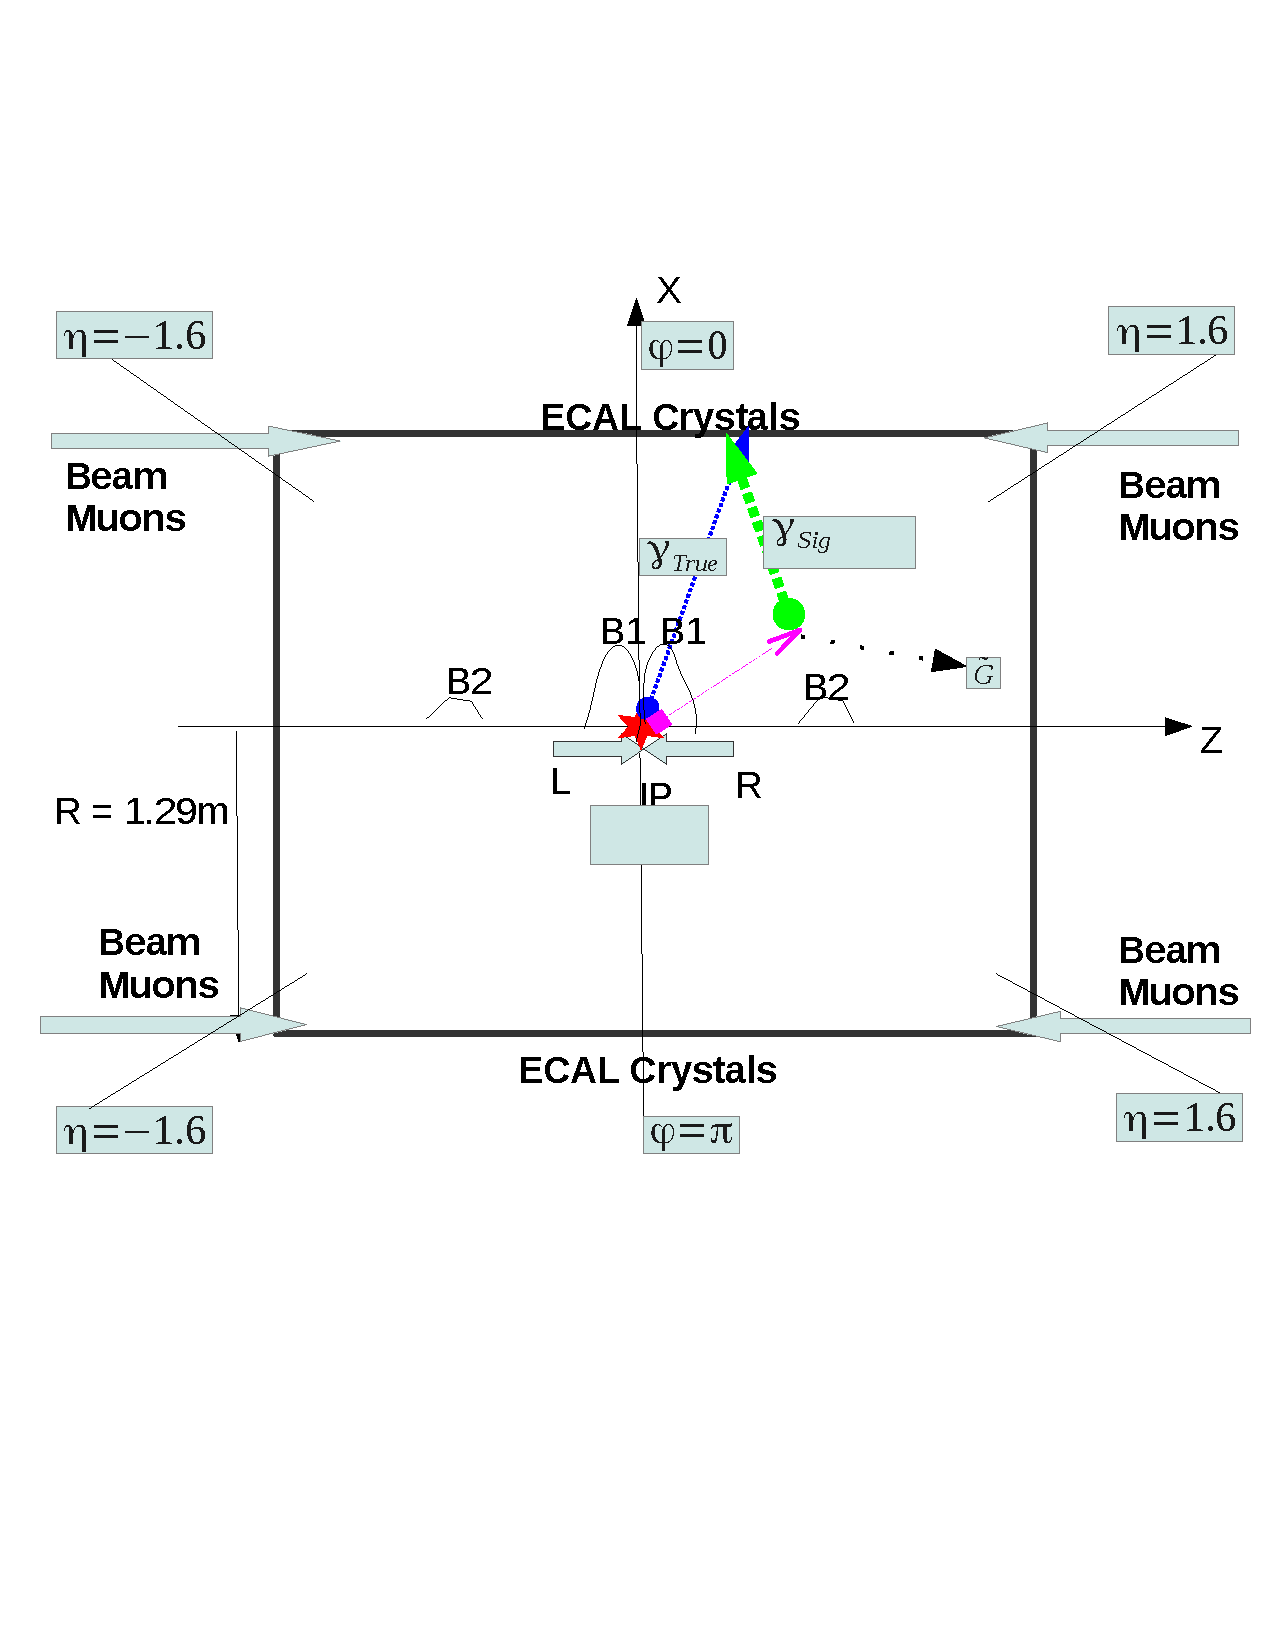
\includegraphics[height=8cm, width=0.5\textwidth]{THESISPLOTS/Background_Delayed_Photon.pdf}
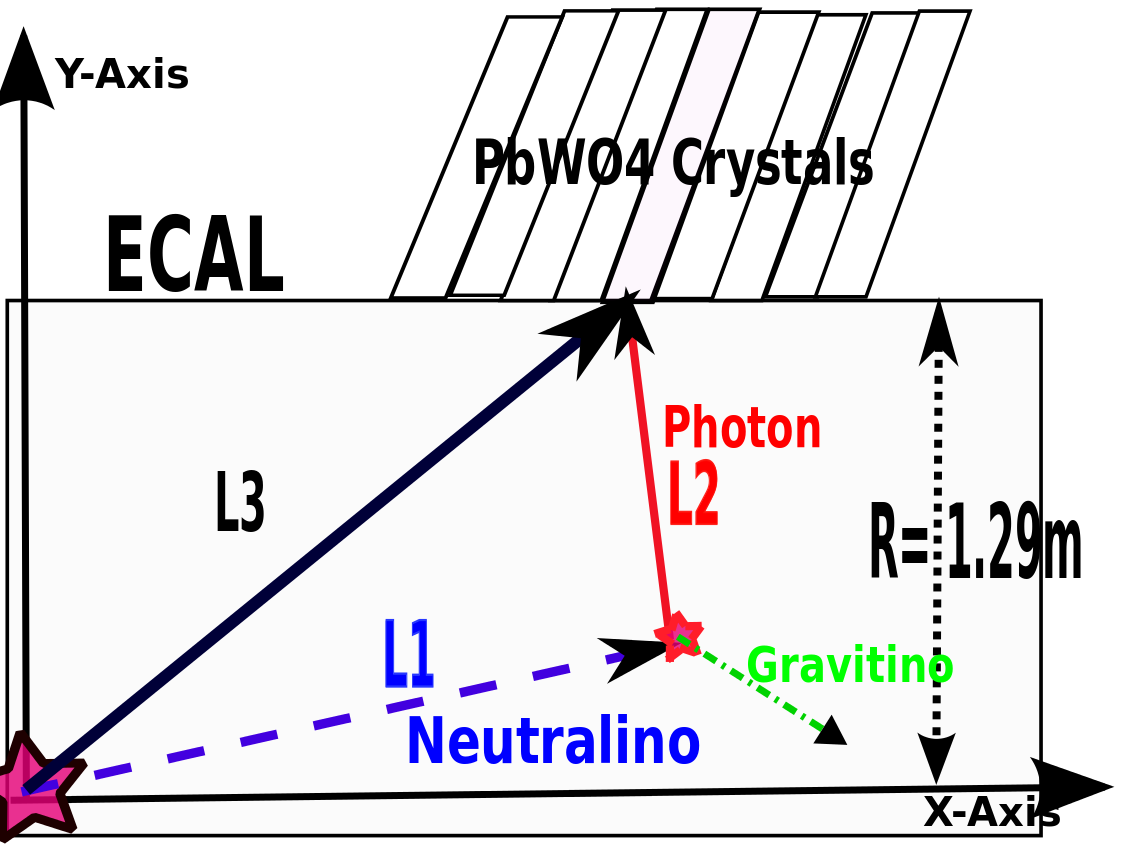
\includegraphics[height=8cm, width=0.5\textwidth]{THESISPLOTS/DelayedPhoton-ECAL.png}}
\captionof{figure}{Schematic diagram showing $\tilde{\chi}^{0}_{1} \rightarrow \gamma + \tilde{G}$ decay topology within the ECAL volume of the CMS detector. Proton beams are also shown showing the possible production of collision and non-collision delayed photons}
\label{fig:NeutDecay}
\end{center}

\subsection{Trigger}
Our pre-event selection begins online be selecting only events which pass our online higher level trigger~(HLT). The HLT trigger used for our $\sqrt{S} = 8$~TeV proton-proton collision analysis is the \texttt{HLT\_DisplacedPhoton65\_CaloIdVL\_IsoL\_PFMET25} 
seeded by \texttt{HLT\_L1SingleEG12} level 1 trigger. It was developed primarily for the study of displaced photons. To avoid bias in event selection towards any particular model, this trigger only requires that an accepted event contains an isolated photon with a \pt threshold of 65~GeV/c and \MET above 25~GeV. The photon shower shape must also satisfy  $ 0.1 < 0.S_{Minor} < 0.4$. We study our trigger efficiency and turn-on curve~(efficiency becomes close to 100\%) for selecting  events with delayed photon candidates. In order to avoid any correlation between the photon and \MET variables, we study efficiency for each variable separately using another trigger \texttt{HLT\_Photon50\_CaloIdVL\_IsoL}.  The selected photon candidates for studying this HLT photon efficiency must pass our offline photon selection candidate criteria shown in table \ref{tab:PhotonSel}. The HLT photon selection efficiency for \pt is defined as the fraction of offline reconstructed photons to those triggered by \textit{HLT\_IsoPhoton50} photon candidates within $\Delta R < 0.5$.
% We do this by using a \texttt{SingleMuon} dataset~(\texttt{HLT\_IsoMu30}) to study the efficiency measurements.
Similarly, the \MET HLT efficiency is defined as the fraction of events containing at least a jet and \MET more than the HLT required \MET of 25~GeV.
The results of the trigger efficiency measurements are shown in figure \ref{fig:HLTEff} against photon \pt and \MET. These efficiency studies are made using the \texttt{HLT\_Photon50\_CaloIdVL\_IsoL} trigger which has no \MET and jet multiplicity requirement  as the denominator and the \texttt{HLT\_DisplacedPhoton65\_CaloIdVL\_IsoL\_PFMET25} as numerator. A \texttt{SinglePhoton} dataset is used to verify these efficiency while and GMSB and $\gamma +$ jets samples is used to derive any correction factors between data and MC events.
\begin{center}
\centering
\mbox{
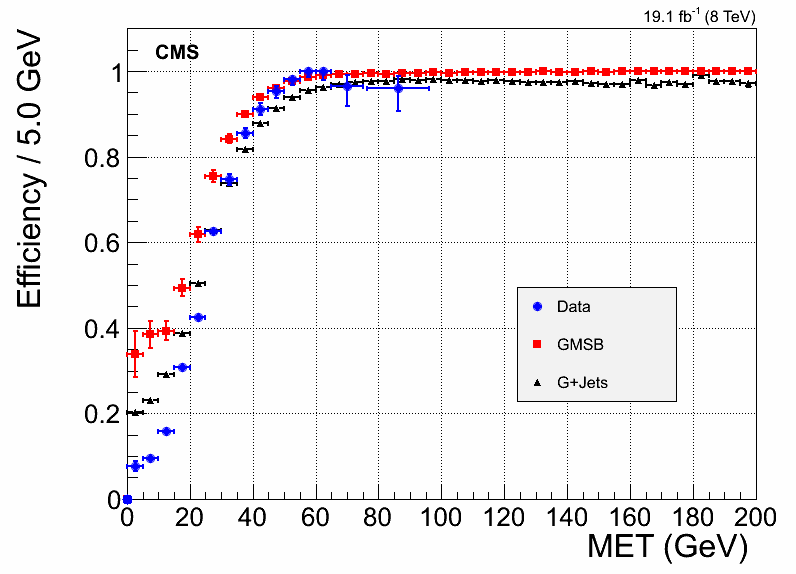
\includegraphics[height=7cm, width=0.5\textwidth]{THESISPLOTS/PFMET_EffAsym.png}
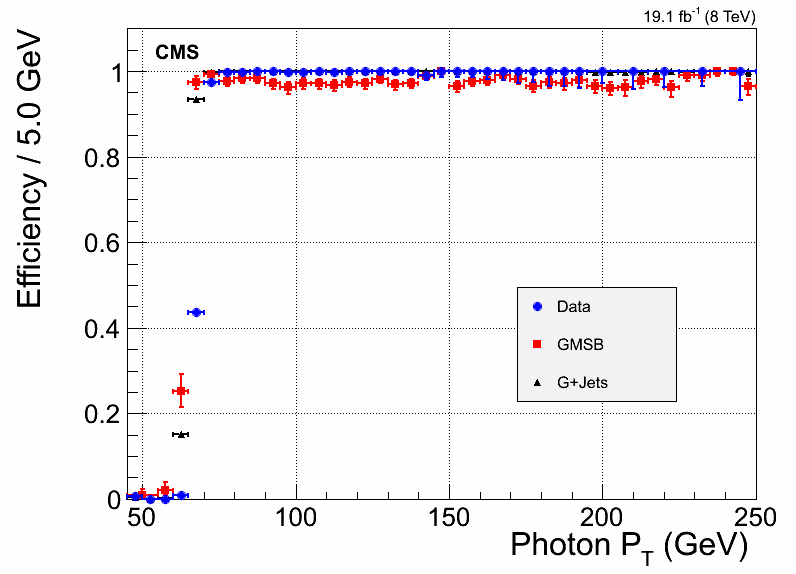
\includegraphics[height=7cm, width=0.5\textwidth]{THESISPLOTS/Photon_EffAsym.png}}
\captionof{figure}{Trigger efficiency turn-on curves for photon \pt and $\MET > 25$~GeV~(left) and for \MET with photon $pt > 80$~GeV/c~(right).The $\gamma +$ jets samples require photon $\pt > 170$~\GeV/c for selecting events with true \MET.}
\label{fig:HLTEff}
\end{center}

\subsection{Offline Selection}
Our offline event selection requires candidate events in addition to passing our HLT trigger, contain at least a single photon, a jet and \MET . The photon object collection used in our analysis is an extended collection of standard CMS Egamma  photon objects collections to include events classified as "\textit{out-of-time}". This classification was performed during the official CMS supercluster reconstruction process. This enlarged  photon sample include events like spikes, ECAL noise, photons from beam halo and cosmic muons and detector malfunctions. It is also entirely possible that this collection also contains true candidate delayed photons which is our signal events.
The selected photons are required to pass the photon selections criteria in table \ref{tab:PhotonSel}. 
\begin{center}
%\begin{table}[ht]
\centering
\begin{tabular}{c c }
\multicolumn{2}{c}{\bfseries{Photon Identification  and Selection Criteria}} \\
  \hline 
  \bfseries{Criteria} & \bfseries{Requirement} \\
   \hline 
 % \texttt{primary vertex number of tracks(vnof)}& $>= 4$ \\
 % \texttt{primary vertex transverse distance to beam}~($d0$) & $ < 2$~cm from CMS center \\
%  \texttt{primary vertex longitudinal distance to beam}~($|z|$) & $ < 24$~cm from CMS center \\
  \texttt{Event leading photon must have} $\pt(\gamma^{1})$  & $ > 80$~ GeV \\
  \texttt{Other photons in event must have} $\pt(\gamma^{>1})$  & $ > 45$~ GeV \\
  
 $|\eta_{\gamma}|$,(\texttt{Barrel Only}),  & $ < 3.0$ ($ < 1.5$) \\
 $S_{minor}$  & $ 0.12 \leq S_{Minor} \leq 0.38$ \\
 \textbf{H/E}  & $ < 0.05$ \\
 
 $\Delta R(\gamma, track)$  & $ > 0.6 $ \\
 
 HCAL Iso  & $ < 4.0 $ \\
 ECAL Iso   & $ < 4.5 $ \\
 Track Iso   & $ < 0.2 $ \\
 Photon Isolation cone size $\Delta R(\gamma, other particle)$ & $< 0.4$ \\
 Topological Spike cuts  & $1 - E_{6}/E_{2} < 0.98$, $ 1 - E_{4}/E_{1} < 0.98$ \\ 
  \hline 
\end{tabular}
\captionof{table}{The photon identification and selection  criteria used in this analysis}
\label{tab:PhotonSel}
%\end{table}
\end{center}

The presence of jets as associated particles from gluino cascade decay
%~(Feynman diagram in figure \ref{fig:ProdDecay} of section \ref{Science_Chapter}) 
 and the gravitino~($\tilde{G}$) from neutralino 
decay, $\tilde{\chi}^{0}_{1} \rightarrow \gamma + \tilde{G}$  requires jet identification and \MET or $\ETslash$~ selection criteria as well.
Our  jet and \MET or $\ETslash$~ selection criteria is based on the particle-flow~(PF) algorithm. Additional $\ETslash$~~$ > 65$~GeV due to the flatness of the HLT trigger efficiency  against \MET ~(see figure \ref{fig:HLTEff}). Table \ref{tab:JetSel} show a summary the jet identification and selection criteria with the threshold requirements used in this analysis.

\begin{center}
%\begin{table}[ht]
\centering
\begin{tabular}{c c }
\multicolumn{2}{c}{\bfseries{Jet PF identification selection criteria}} \\
  \hline 
  \bfseries{Criteria} & \bfseries{Requirement} \\
   \hline  
\texttt{Jet} \pt & $ > 35$~GeV \\
 \texttt{Number of Jet constituents} & $ > 1$ \\
 \texttt{Charge EM energy fraction~(CEF) } & $ > 0.99$ \\
 \texttt{Neutral Hadron energy fraction~(NHF) } & $ < 0.99$ \\
 \texttt{Neutral EM energy fraction~(NEF) } & $ < 0.99$ \\
 \texttt{If} $|\eta|$ \texttt{of jet is} $ >2.4$, \texttt{Charge Hadron energy fraction~(CHF) } & $ > 0$ \\
 \texttt{If} $|\eta|$ \texttt{of jet is} $ >2.4$, \texttt{Charge multiplicity~(NCH) } & $ > 0$ \\
 $\Delta R(\gamma, jet) = \sqrt{(\phi_{\gamma}-\phi_{jet})^{2} + (\eta_{\gamma}-\eta_{jet})^{2}}$ & $ > 0.3$ \\
\hline
\end{tabular}
\captionof{table}{The Jet ID selection used in this analysis}
\label{tab:JetSel}
%\end{table}
\end{center}

\paragraph*{\MET Corrections}\mbox{}\\
During the official CMS electromagnetic supercluster reconstruction, timing cuts of $|t_{RECO}| > 3.0$~ns in EB is used for cleaning "out-of-time" events. As a result, the \pt contribution from out-of-time photon events is not included in the calculation of \MET or $\ETslash$~~. This introduces a difference in the calculation of $\ETslash$~~ for "in-time" events~($|t_{\gamma}| < 3.0$~ns) and "out-of-time" events~($|t_{\gamma}| > 3.0$~ns). Since the out-of-time photon \ET is not included in the sum total transverse momentum of an event to derived the total transverse momentum imbalance, we correct for this, by adding the out-of-time photon $\ET$ to the PF-MET measured during CMS $\ETslash$~~ reconstruction. We defined an additional variable, ${\ETslash}^{\gamma}$ , accounting for this correction and use this variable in our event selection criteria. 
\begin{enumerate}
\item ${\ETslash}$~ : PF-MET, $\ETslash$~~  from CMS standard \MET measurements.
\item ${\ETslash}^{\gamma}$~: PF-MET with photon \ET added i.e ${\ETslash}^{\gamma} = \ETslash\quad + ~\et$ of the  out-of-time photon.
 \end{enumerate}
%The distributions for ${\MET}_{1}$ and ${\MET}_{2}$  against ECAL time can be seen in figure \ref{fig:METS}.

%\begin{center}
%\centering
%\mbox{
%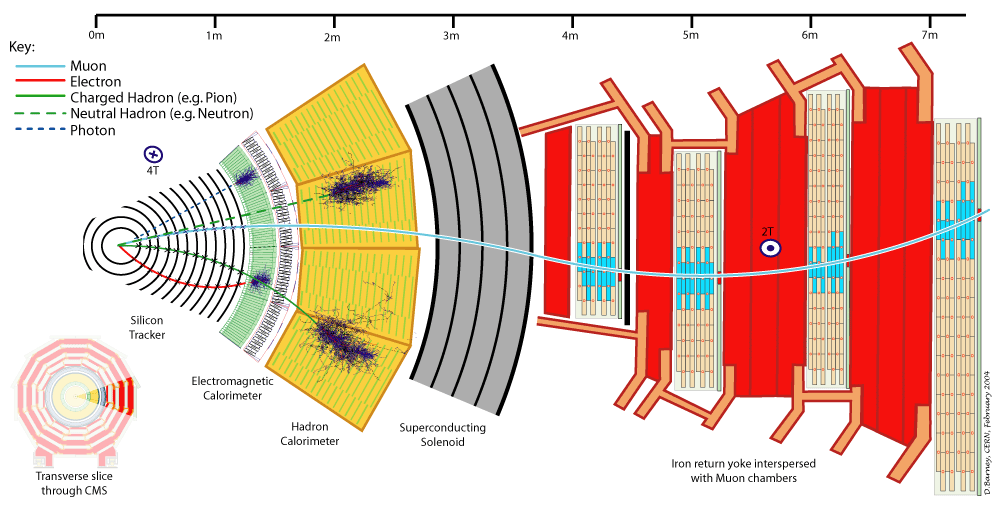
\includegraphics[scale=0.2]{THESISPLOTS/CMS_Slice.png}
%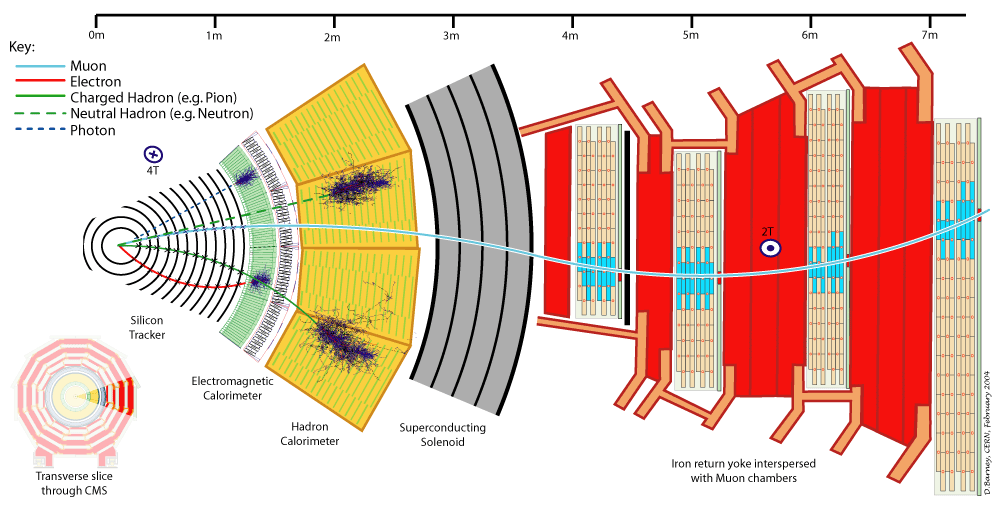
\includegraphics[scale=0.2]{THESISPLOTS/CMS_Slice.png}
%\captionof{figure}{Figure showing \MET distributions for events with out-of-time and in-time photons. ${\MET}_{1}$ and ${\MET}_{2}$ definitions are given in context. }
%\label{fig:METS}
%\end{center}

Our signal event selection criteria is defined as events with  $\ge1~\gamma  + \ge2~ jets + {\ETslash} > 60$~GeV $ + {\ETslash}^{\gamma}~ > 60$~GeV 

We use a control sample to perform a closure test of our background estimation procedure. The selection criteria is events with  $ \ge1~\gamma + \le1~jet  +  {\ETslash}~ > 60$~GeV $ + {\ETslash}^{\gamma}~ > 60$~GeV 

\subsection{ECAL Time}
The photon arrival time at ECAL is our main observable for distinguishing background from signal.  However, the presence of spikes, noisy crystals and pile-up events, require measuring the photon time with methods which are robust to timing bias from such events.
There are different ways to measure the photon time using ECAL.  The reference time is the time measured from a relativistic electromagnetic object like a photon produced from nominal proton-proton collisions arriving at ECAL in an average time of zero. The photon time is measured using either of the following methods: 
\begin{itemize}
\item \textit{Seed Time}: Time from the highest energy crystal, which is not a spike, of the photon supercluster.
\item \textit{Cluster Time}: Error weighted average time of all the crystals in the seed basiccluster of the photon supercluster.
\end{itemize} 

Timing reconstruction as described in chapter 4 is the extraction of time from the pulse shape through a fitting method. The $\chi^{2}$ obtained from the fit determines how well the time is reconstructed. One way of rejecting fake photons which are either jets miss-identified as photons or spikes is to use the fitted $\chi^{2}$. Studies performed have shown that a  $\chi^{2} < 4 $ cut improves the ECAL timing resolution by rejecting  spikes and anomalous photon events as possible. Figure \ref{fig:spikeVsPhoton} shows a comparison between the pulse shape profile of a spike and that of a good event.

\begin{center}
\centering
%\mbox{
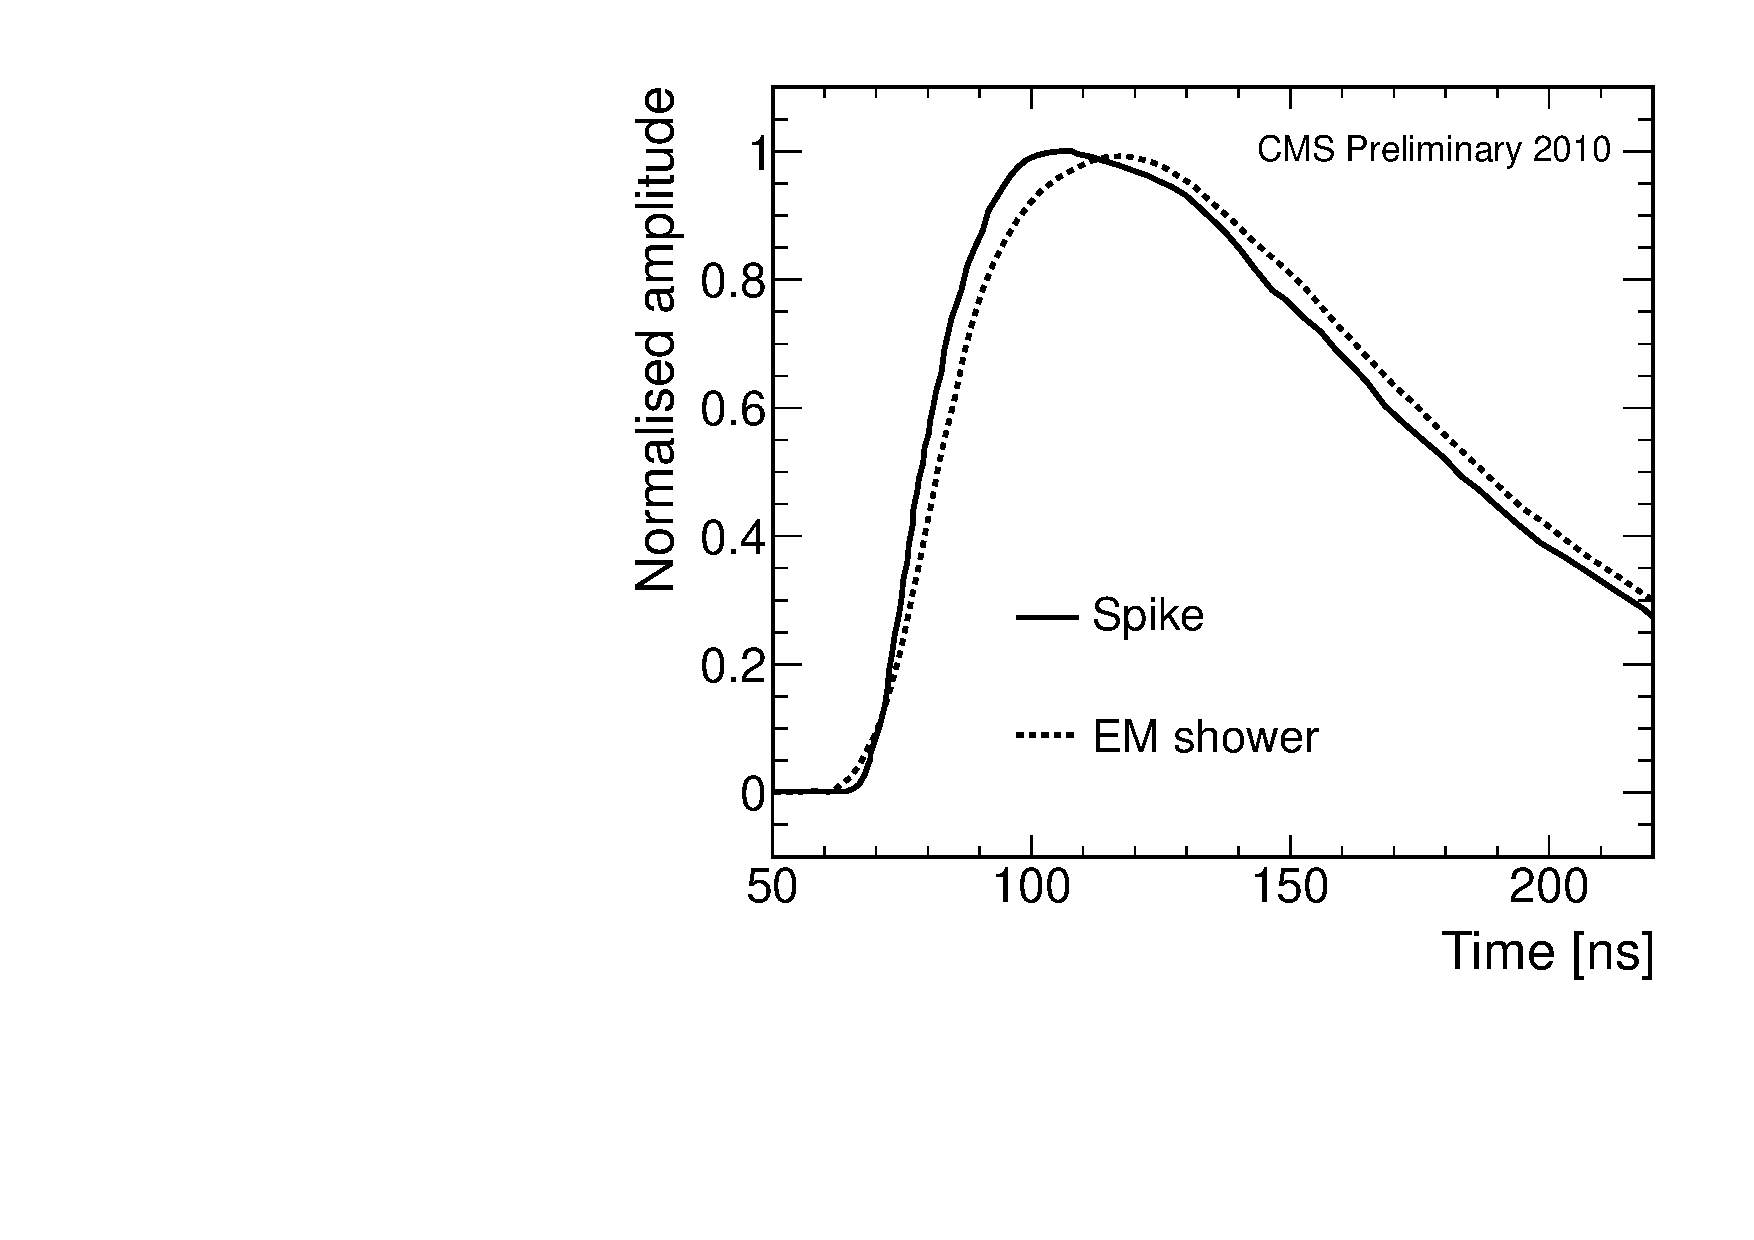
\includegraphics[height=6cm, width=0.7\textwidth]{THESISPLOTS/spike_pulse_shape.pdf}
\captionof{figure}{Pulse shape profile showing a spike~(solid line) and a real photon~(dashed line) from data.}
\label{fig:spikeVsPhoton}
\end{center}.

In this thesis, we measure time using the seed crystal time approach. Our choice of seed time is based on a number of independent timing analysis performed comparing the timing resolution obtained from cluster time to the seed time. We observed the cluster timing method to be very biased towards the time of an isolated spike especially when the spike is embedded in a photon object. The timing resolution especially for large timing events is much better compared to the cluster time measurement method which is an essential region when searching for new long-lived particles.
Figure \ref{fig:TIME} shows the timing measurements of photons using either seed time or cluster time. The seed time show an approximate timing resolution of $400$~ps compared to $450$~ps with a broad timing tail from using the error weighted average cluster time. The cluster time method is also computational time and resource consuming.

\begin{center}
\centering
\mbox{
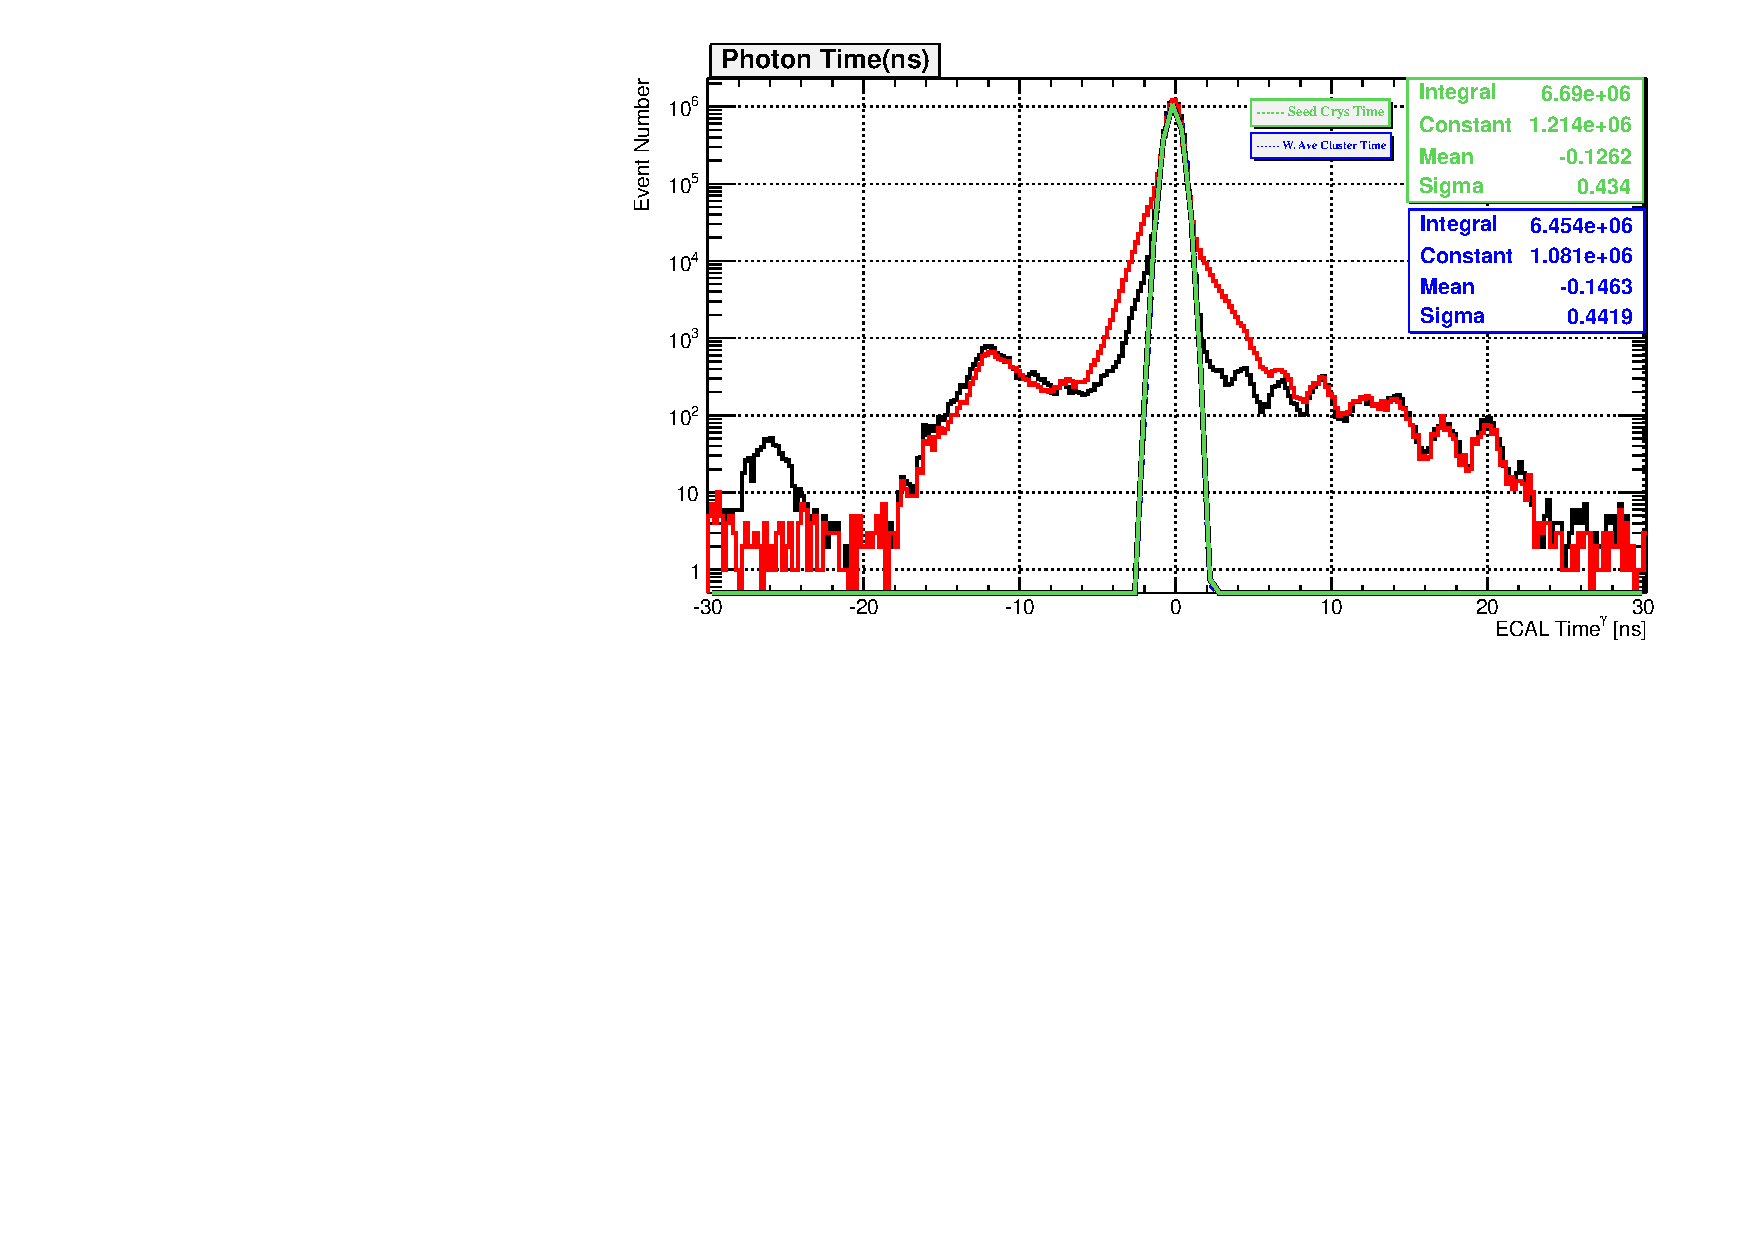
\includegraphics[height=6cm, width=0.5\textwidth]{/home/tensr/Documents/TEN-HEP-PHD-THESIS/PHD_THESIS/PHD/THESISPLOTS/SeedTimeVsWAveBasicClusterTimeDefinitions.pdf}
%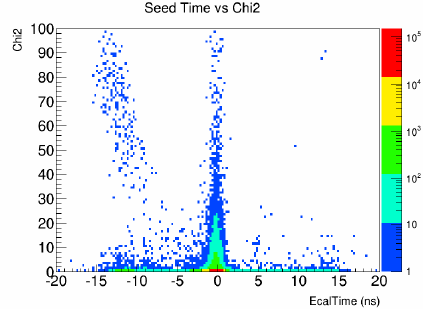
\includegraphics[height=6cm, width=0.5\textwidth]{THESISPLOTS/Seed-Time-Chi2.png}
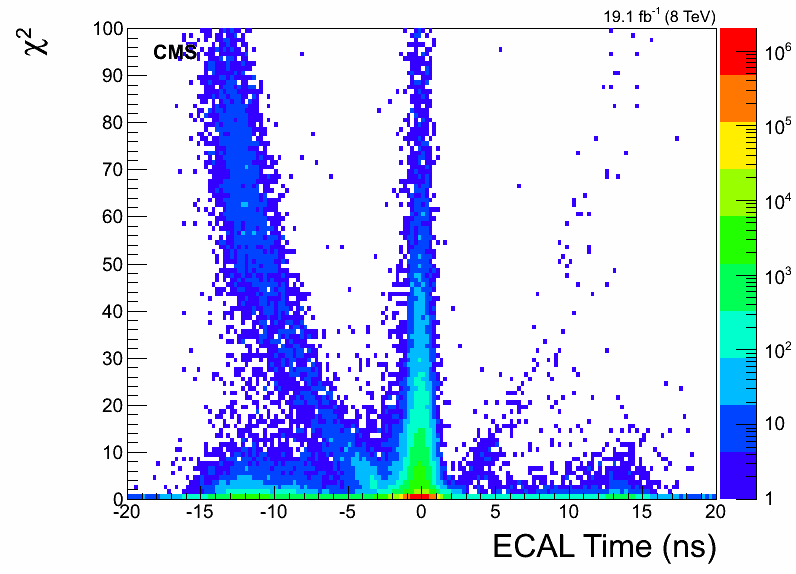
\includegraphics[height=6cm, width=0.5\textwidth]{THESISPLOTS/seedTime_Chi2.png}
}
\captionof{figure}{Timing distribution of photons  showing timing measurements using seed crystal~(black) and using Weighted Average basic cluster time~(blue). Resolution~($\sigma$) from seed time is better compared to that for cluster time which is computationally intensive. Together with the $\chi^{2}$, the seed time performs better in identifying anomalous timing objects.}
\label{fig:TIME}
\end{center}

Monte Carlo simulation of ECAL timing is challenging  as the time of anomalous events such as spikes and noisy crystal channel  present during data taking 
aren't well simulated.  To account for MC and data timing measurement differences, 
We use QCD simulated $\gamma + jets$ events and select events containing only one or two jets and study the distribution of the difference between the generated time~$(T_{GEN}$) and the reconstructed MC event time~($T_{RECO}$) in a timing window of [-2, 2 ]~ns. Comparing this difference to data, the difference in the mean time between the data and MC $\gamma +$ jet sample is used to smear the reconstructed time of the MC samples to be comparable to true reconstructed time in data. A difference of about 125~ps is observed between the timing from data and MC.  Timing from the smeared MC sample show a close agreement with data.
Figure \ref{fig:DATAMCTime} show this comparison before and after timing calibration~(smearing adjustment) is applied on the MC samples.

\begin{center}
\centering
\mbox{
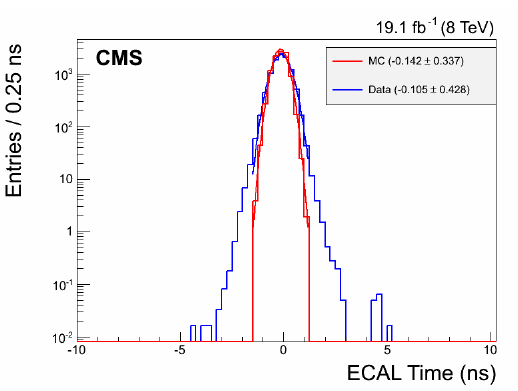
\includegraphics[height=6cm, width=0.5\textwidth]{THESISPLOTS/MC_Vs_DataTimeB4Calib.png}
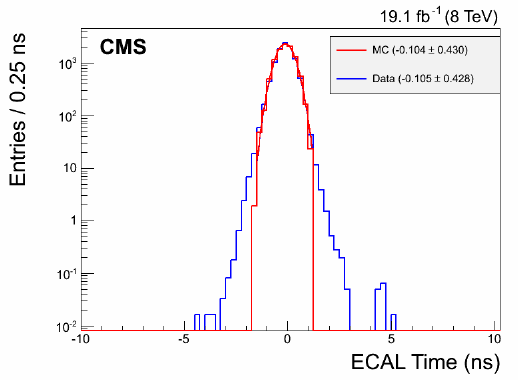
\includegraphics[height=6cm, width=0.5\textwidth]{THESISPLOTS/MC_Vs_DataTimeAferCalib.png}
}
\captionof{figure}{Timing distribution of photons showing timing of data and MC $\gamma +$ jets~(blue) samples and data~(red) before~(left) and after~(right) timing Calibration is applied to MC.}
\label{fig:DATAMCTime}
\end{center}
It is worth noting that the difference of 125~ps between $T^{MC}_{RECO}$ and $T^{DATA}_{RECO}$ compared to 500~ps ECAL timing resolution is not enough to influence event selection, however event distribution in the tails remains a major concern.
\paragraph*{}
The ECAL timing distribution for photons with $pt > 50$~GeV in the ECAL~(barrel and endcap inclusive i.e $|\eta_{\gamma}| < 3.0$) show timing distributions~(see figure \ref{fig:TIMEECAL})

\begin{center}
\centering
\mbox{
%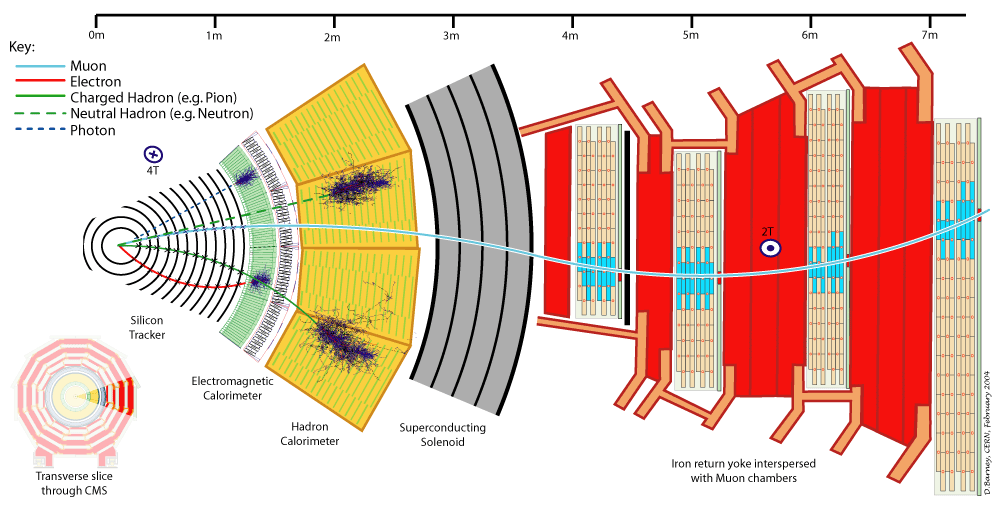
\includegraphics[scale=0.2]{THESISPLOTS/CMS_Slice.png}
%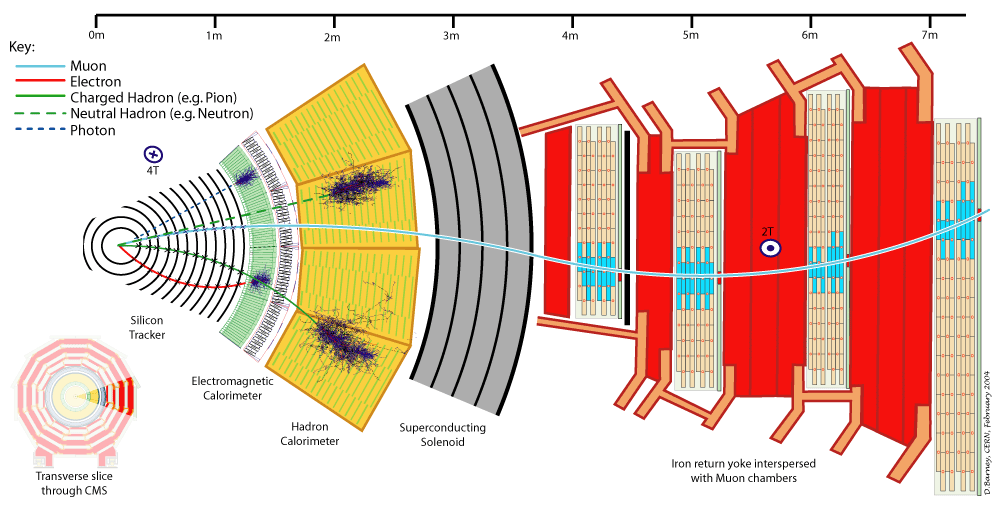
\includegraphics[scale=0.2]{THESISPLOTS/CMS_Slice.png}
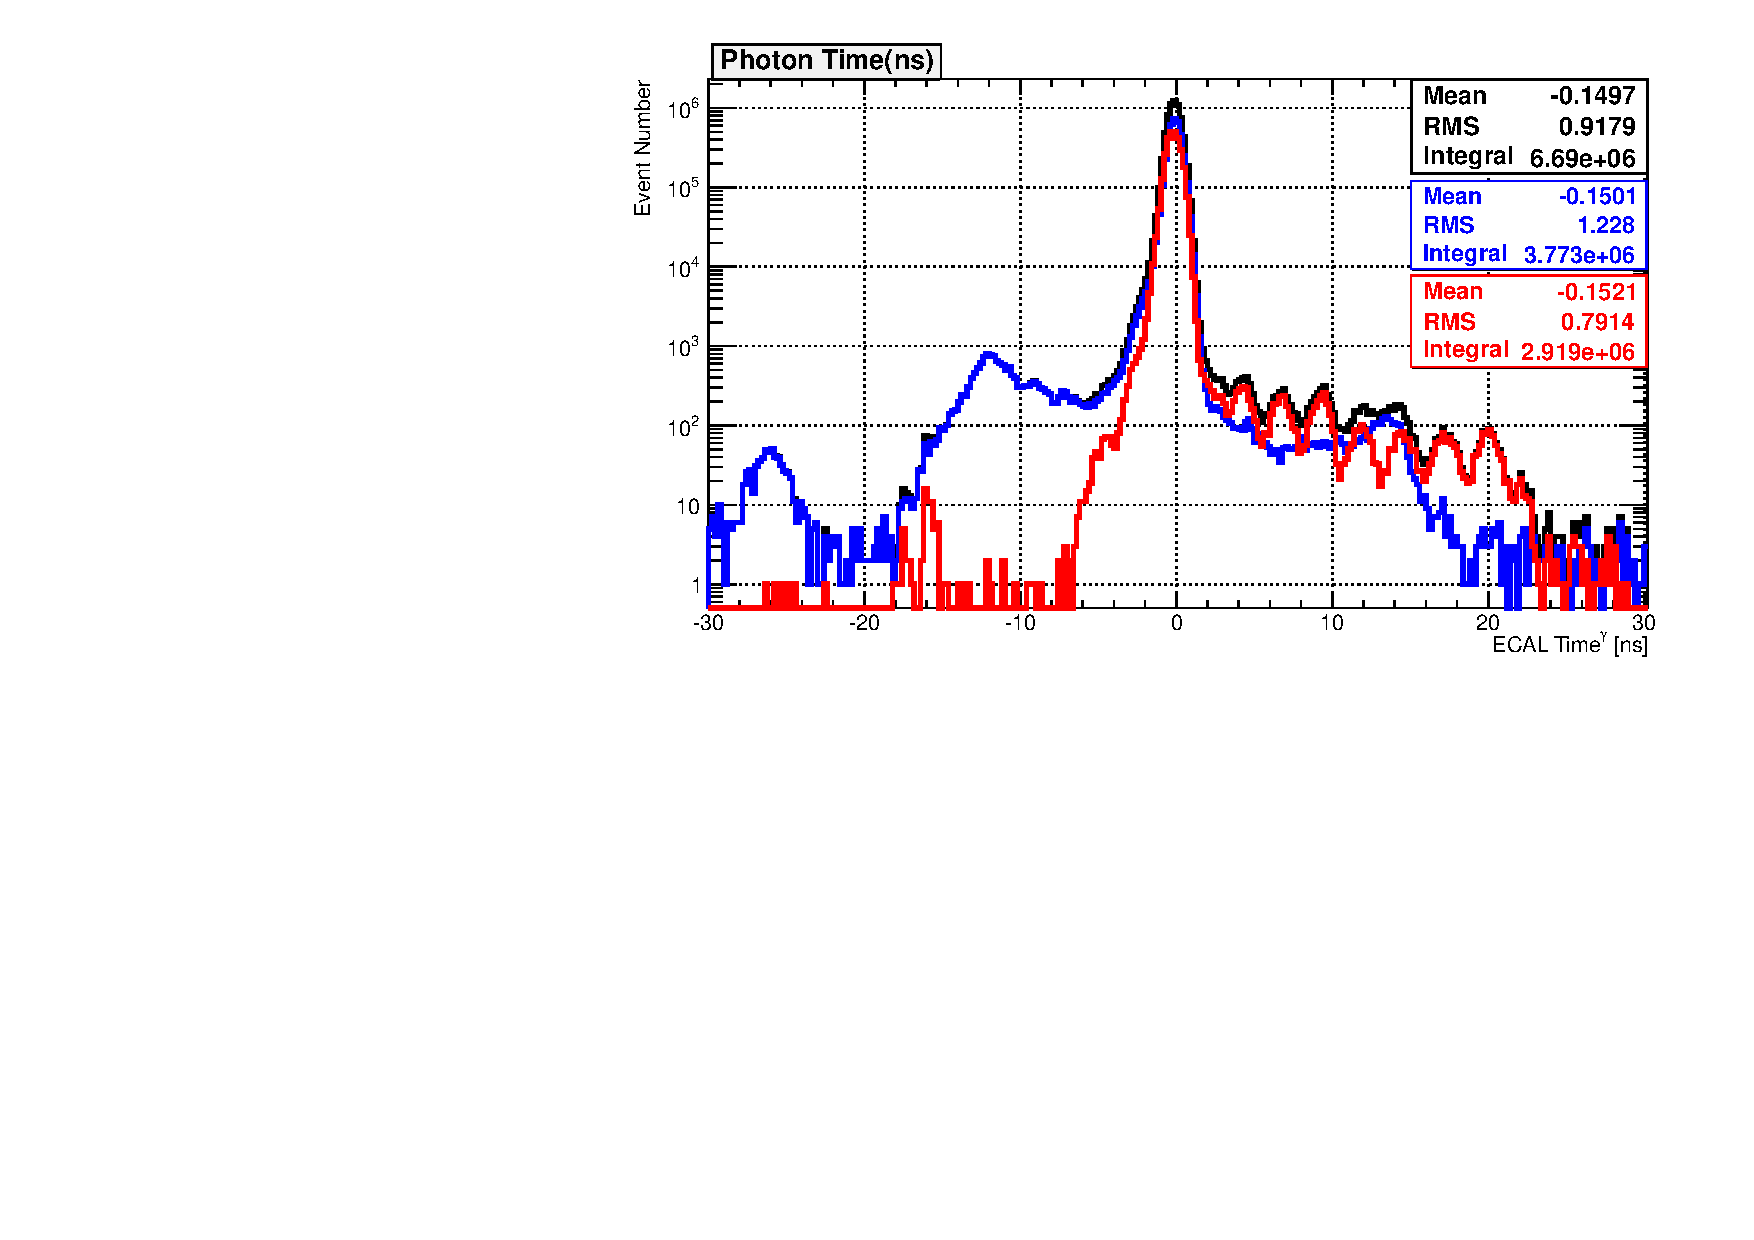
\includegraphics[height=8cm, width=0.9\textwidth]{THESISPLOTS/PhotonECALTimePtMTH50-C-D-SinglePhotonDataset.pdf}
}
\captionof{figure}{ECAL timing distribution of photons in barrel~(\textcolor{blue}{EB}), endcap~(\textcolor{red}{EE}) and all of ECAL~(\textcolor{black}{ALL ECAL}) with $\pt > 50$~GeV from data. A $2.5$~ns delay timing structure is observed in endcap subdetector.}
\label{fig:TIMEECAL}
\end{center}
with a clear 2.5~ns discrete pattern with most of these photons arriving in the endcap, $ 1.47 < \eta < 3.0$ compared to the barrel, $|\eta| < 1.47$. These are photons produced from collisions of \textit{Ghost} and \textit{Satellite} bunches with either the main proton collision bunch or \textit{Ghost}/\textit{Satellite}. They contribute an irreducible amount to the photon time distribution which is very challenging to reject or estimate quantitatively. A rough estimate can be obtained by looking at ratio of the proton population in the filling profile of the LHC RF cavities as mentioned in section 3.1.5 of chapter 3 which gives a factor $10^{-5}$ compared to contributions from the main proton-proton bunch collision. It is observed that contribution from ghost bunches is in the endcap crystals, since very few these photons are produced with enough \pt compared to those from main proton bunch collisions. And even if they dis, the ratio of photons from these secondary proton collision to that of the main proton-proton collision is of the order of $10^{-5}$ at most. 
As a result of this, we do not used the endcap in this analysis in addition to the fact that timing resolution in the endcap is relatively poor compared to the barrel.
We check and validate this factor $10^{-5}$ using events with $Z\rightarrow \EE$ since $Z$ events do not require high \pt during production and must should capture the 2.5~ns timing pattern if present from ghost/satellite collisions. We study electron candidates with time within [-2.0, 2.0]~ns window. We use this in our background estimation method testing as will be discussed in future sections.

\paragraph*{Delayed Photon Source} \mbox{}\\
With a well time calibrated ECAL and good  MC to data time agreement, we can study the source of delayed photons from neutralino decay in ECAL using its decay kinematics. There are two possible sources for delayed photon from neutralino decay.
From Figure \ref{fig:NeutDecay}, an estimated photon arrival time at ECAL can be given by the following methods:
\begin{itemize}
  \item From slow moving neutralinos: $\Delta t_1$ = (L1/c$\beta$) - (L1/c)
  \item From non-directpath traveled: $\Delta t_2$ = (L1 + L2 - L3)/c
  
  \item ECAL measured time = $\Delta t_{1} + \Delta t_{2}$
\end{itemize}
 
Figure \ref{fig:DELAY} shows the distribution of $\Delta t_{1}$ and $\Delta t_{2}$
indicating that most of our late arrival photons are produced from the decay of slow moving neutralinos, \ie $\beta << 1$,  as opposed to photons from non-direct flight or travel path to ECAL. These neutralinos are produced with low \pt such that the ratio $\frac{\pt}{m_{\tilde{\chi}^{o}_{1}}} << 1$.


\begin{center}
\centering
\mbox{
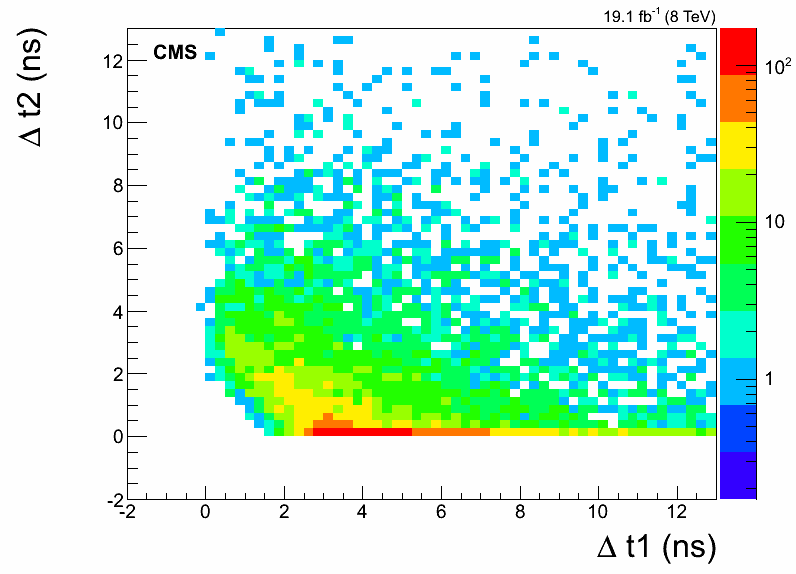
\includegraphics[height=6cm, width=0.7\textwidth]{THESISPLOTS/dt1_dt2_late.png}}
\captionof{figure}{Sources of delayed photons produced from neutralino decay in the SPS8 model with $\Lambda= 180$~TeV and $c\tau = 6000$~mm arriving at ECAL.}
\label{fig:DELAY}
\end{center}

\section{Background Estimation}
Our background estimation strategy is to first identify and reject as much non-collision background and anomalous events as possible then perform an ABCD background estimation technique on the irreducible residual background. We do this by comparing photon kinematic properties for in-time and off-time photon events. Separating our data sample into jet multiplicity and negative, in-time and positive time enable our approach to be possible. To better understand the different background sources and their contribution we make a two dimensional histogram of the photon $\eta$ and $\phi$ against the photon seed time  and a one dimensional histogram of the timing distribution for different jet multiplicity events. These events pass the loose selection criteria for photons, jets and $\ETslash$~~ already described in the previous section.
The photon ECAL time  Vs $\eta$ and $\phi$ inclusive 2-D distributions are shown in figure \ref{fig:BKGPLOTS}
\begin{center}
\centering
\mbox{
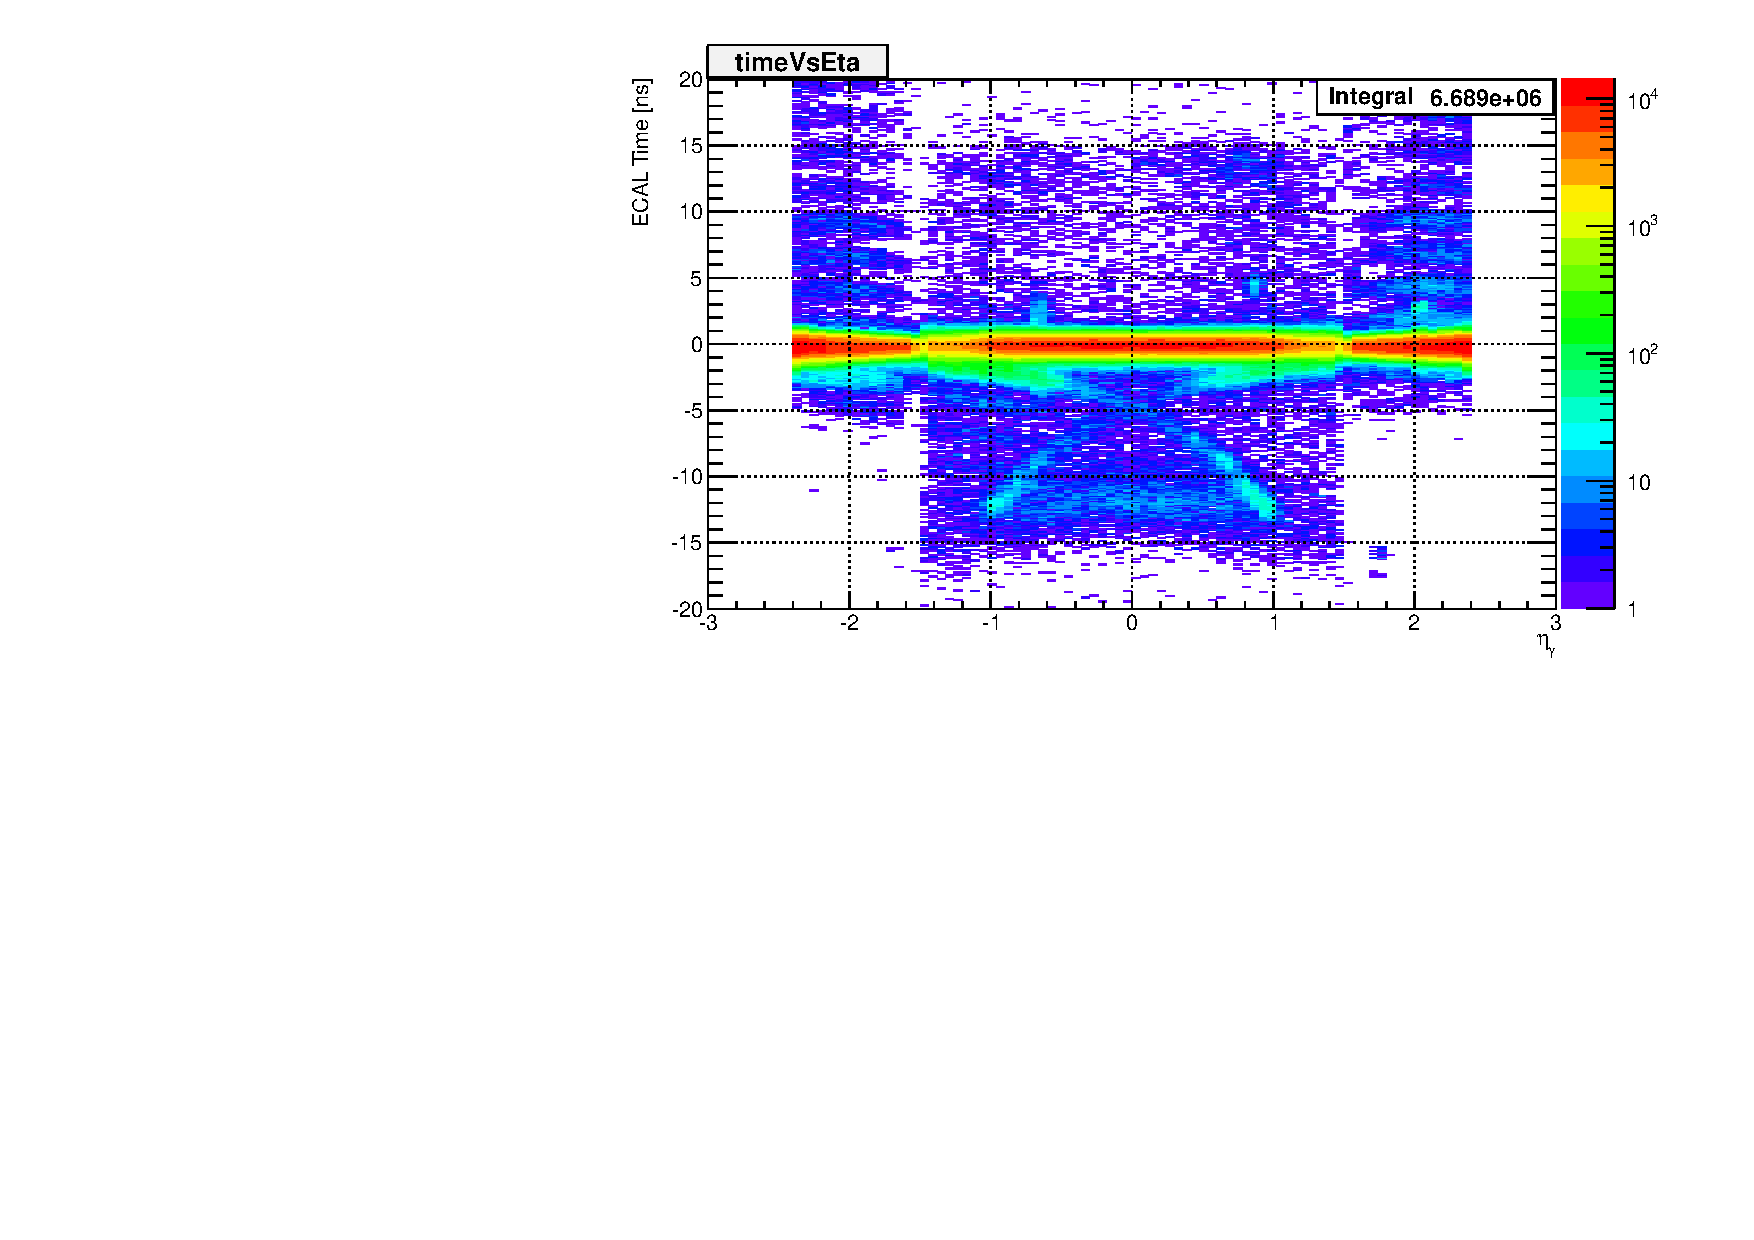
\includegraphics[height=6cm, width=0.5\textwidth]{THESISPLOTS/SinglePhotonDataSet-TimeVsEta.pdf}
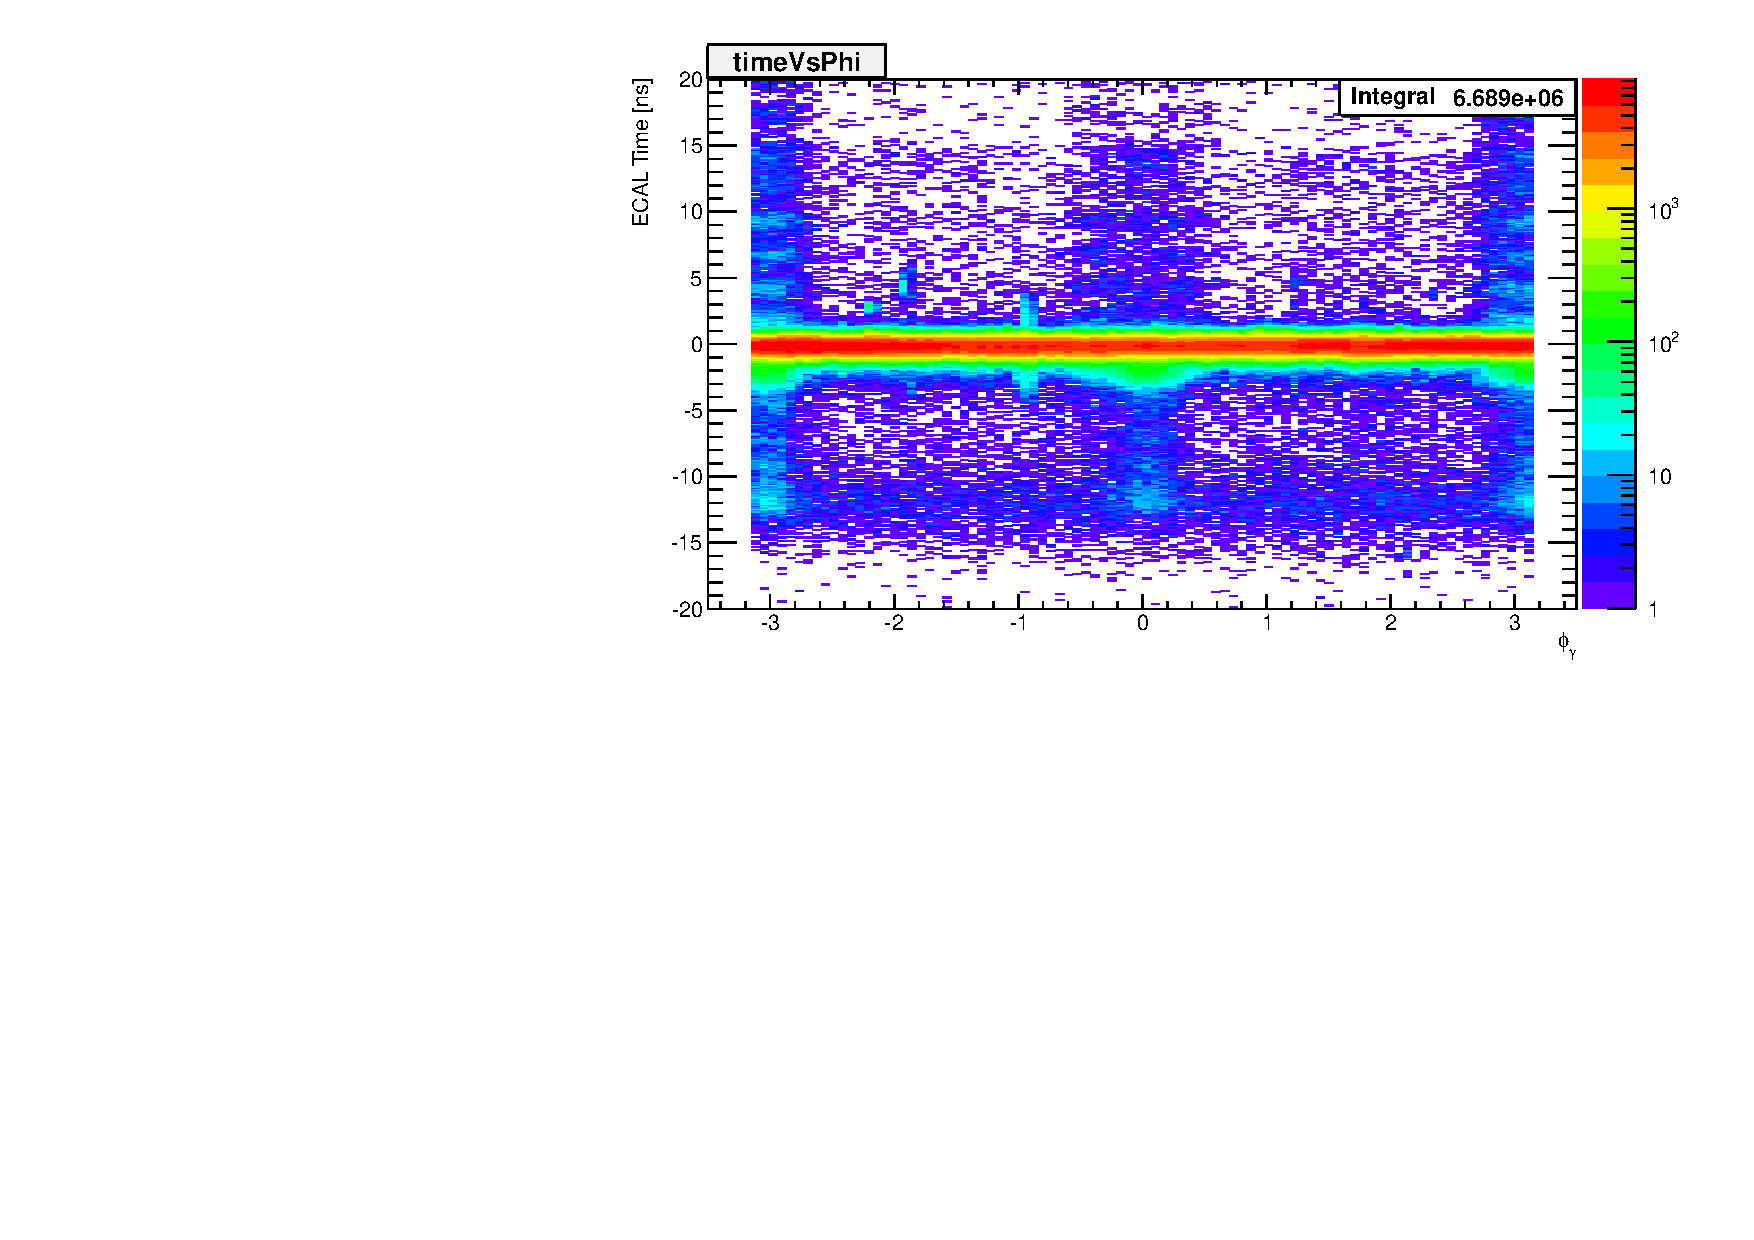
\includegraphics[height=6cm, width=0.5\textwidth]{THESISPLOTS/SinglePhotonDataSet-TimeVsPhi.pdf}}
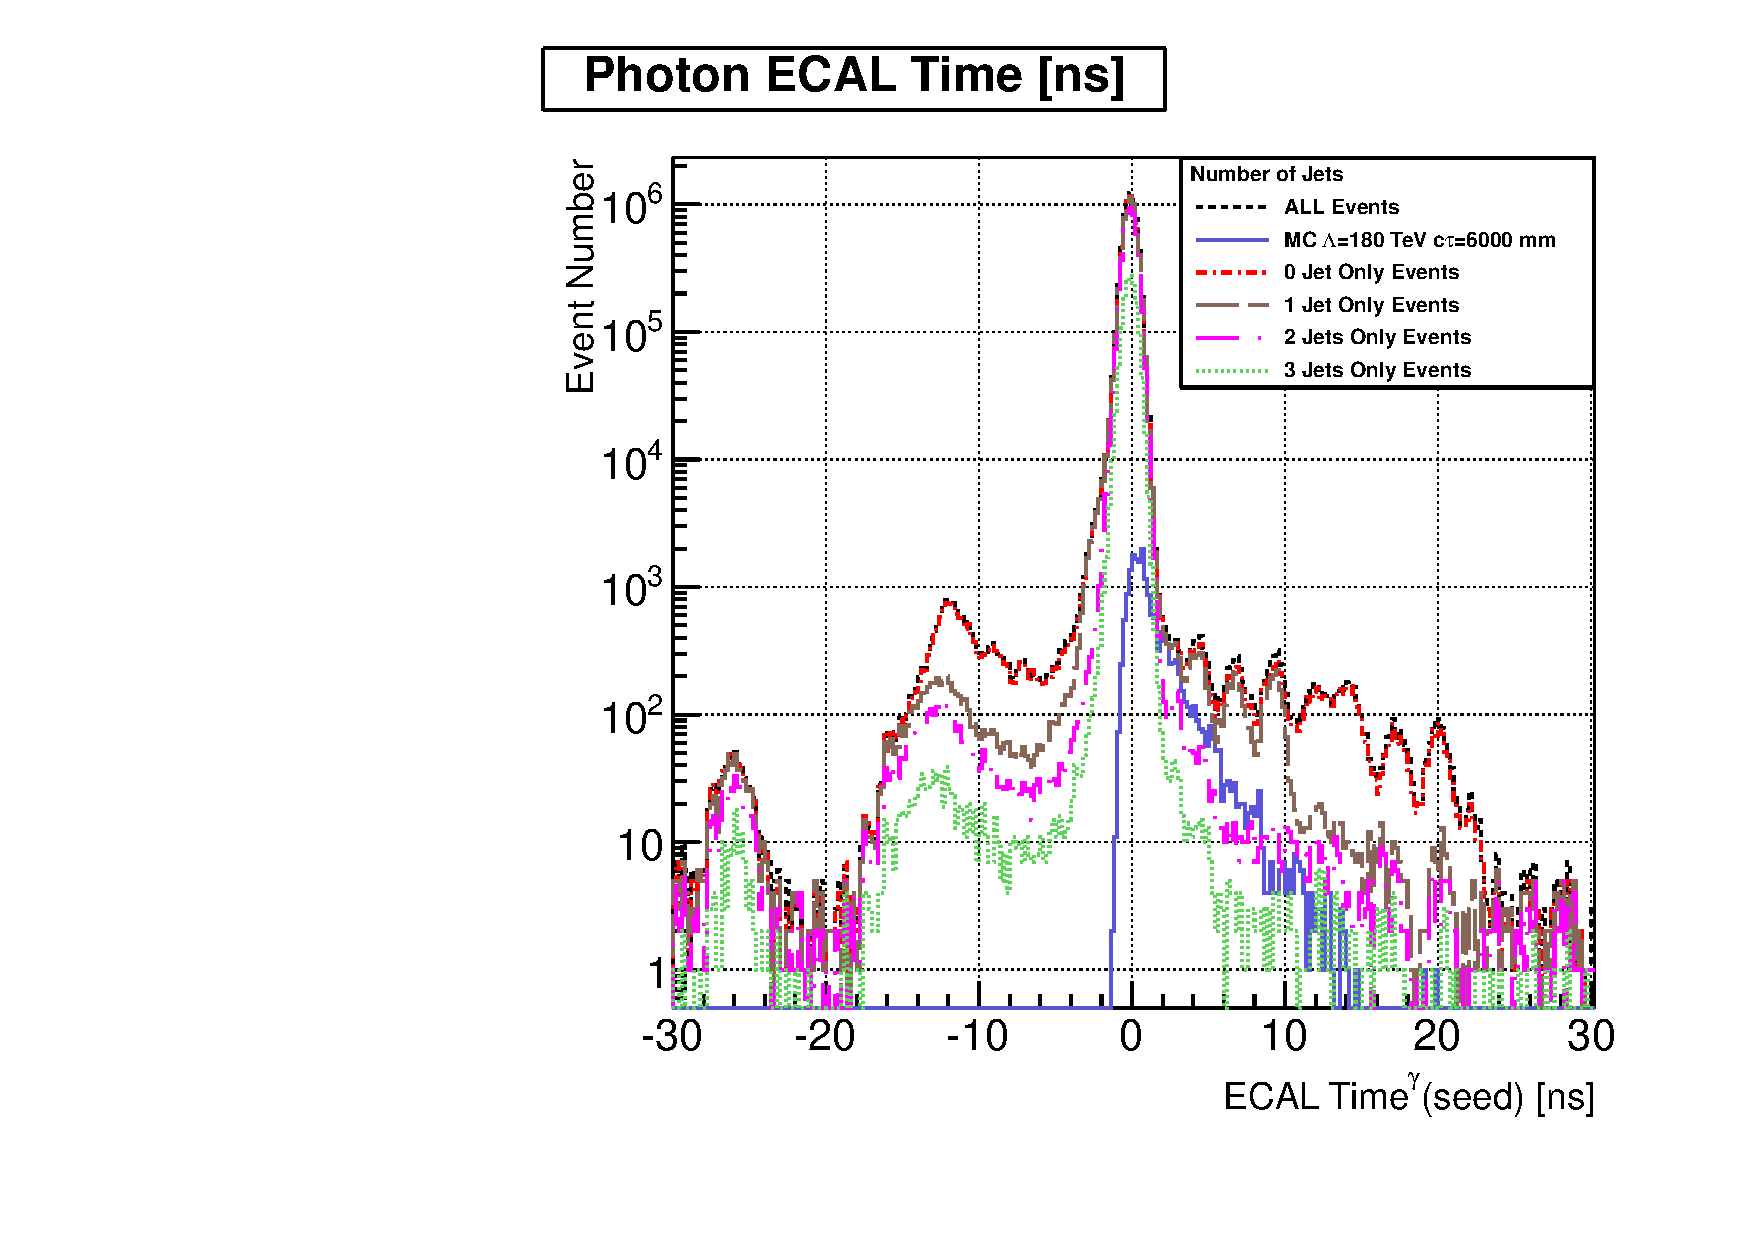
\includegraphics[height=8cm, width=0.8\textwidth]{THESISPLOTS/Photon_SeedXtalTime_Distribution_VsJetMultiplicity.pdf}
\captionof{figure}{ECAL time against $\eta$~(left) and ECAL time against $\phi$~(right) for photons with $\pt > 60$~GeV from data. The lower plot shows the photon timing distribution for events with different jet multiplicity.}
\label{fig:BKGPLOTS}
\end{center}
The histograms in figure \ref{fig:BKGPLOTS} show contributions from quite a variety of sources. The possible sources considered in this analysis include: QCD processes which we consider to be a combination of $\gamma + $jets, multijets and other processes producing photons from nominal proton-proton main bunch collisions. Most of the QCD processes are expected to have minimal contribution to large timing photons and $\ETslash$~~ except due to timing miss-reconstruction and $\ETslash$~~ miss-measurements or miss-identification of jets as photons.
The events with significant contributions of possible or true large ECAL time measurements are produced from machine induce backgrounds~(MIB)(arising from ghost/satellite bunch collisions) or beam halo muons, cosmic muons and anomalous events like spikes. These event do not only contribution significantly large photon times but also to large $\ETslash$~~ which is our signal selection sample.
We employ a data driven background estimation technique in this analysis described briefly as follows:

\begin{itemize}
\item Divide the dataset into individual samples peculiar to the expected kinematics and observation of each individual background source,
\item Identify observable based on its kinematics which can be used as variables to identify or tag and reject a particular background contribution with an acceptable amount of efficiency,
\item Used alternate samples particular to each background source to calculate and verify the event tagging and miss-tag rate or efficiency,
\item Use the tagging and miss-tag rates to estimate the background contribution of each individual background source in a well defined control region~(CR) or sample,
\item Use another CR as a closure test sample to verify our background estimation method.
\end{itemize}
All events are selected to be in the barrel i.e $|\eta_{\gamma}| < 1.47$ as the
the overwhelming contribution of ghost/satellite bunch collisions observed in the endcap~(EE)(see figure \ref{fig:TIMEECAL}) and poor timing resolutions~($\approx 3.0$~ns) make it very challenging to extend this analysis to include the endcap~(EE). 
Our data driven method background estimation strategy involves splitting our single photon dataset into two major samples: Events with \textit{Nominal or in-time} photons whose photon ECAL time is within $\pm 2$~ns containing at least $2$ jets,  and events with \textit{off-timing} photons where the photon ECAL time is $ 2.0 < t_{\gamma} < 13.0$~ns and $ -10.0 < t_{\gamma} < -3$~ns with containing $0$ or $1$ jets.  Our signal events are events containing photon(s) with ECAL time, $ 2.0 < t_{\gamma} < 13.0$~ns, with at least $2$ jets and large $\ETslash$~~. Our motivation is to avoid the observed spike overpopulated region with photon time , $t_{\gamma} \approx -12$~ns and because high jet multiplicity events are not usually MIB or non-collision events produced with \pt.
On the other hand, nominal photons from QCD interaction are mostly produced in-time in association with more than $0$ jets.

By comparing these two samples, we develop kinematics variables for studying and reducing contributions from collision and non-collision backgrounds. 

\subsection{Non-Collision Backgrounds}
\subsubsection{Halo Photons}
Muons with energy up to 1 TeV are produced when proton beam collides with collimators at $z = 150$~m from the CMS detector interaction point or when proton beams collide with residual beam gas in the beam pipes. These are referred to as  Beam-Induced Backgrounds~(BIB). These muons through the process of bremsstrahlung produce high \pt photons with significantly large ECAL time, deposit their energy in ECAL crystals. The rate of BIB produced photons depend on the beam current and the operational conditions of the LHC such as machine optics, collimator settings, residual gas densities and filling scheme. These muons which travel in a near parallel flight path to the direction of main proton bunch in the beam pipe are referred to as \textit{halo muons}. We expect halo muons to produced muon tracks in the Endcap muon systems~(CSC and RPCs) with corresponding associated ECAL electromagnetic cluster in the ECAL. Halo muons can travel from one side of the detector, along the $z$-direction, to the other side of the detector if produced with sufficient energy. Their Time-Of-Flight~(TOF) with respect to a potential hit position in the ECAL sub-detector can be estimated and measured.
The expected arrival time at ECAL of a halo muon traveling parallel along the beam line is estimated using it kinematics given in equation \ref{eq:HALOPATH}.

\begin{equation}{\label{eq:HALOPATH}}
t^{\mbox{expected}}_{\mbox{ECAL}} = -1/c\left( \pm Z_{\mbox{cluster}} + \sqrt{Z^{2}_{\mbox{cluster}} + R^{2}_{\mbox{cluster}}}  \right)
\end{equation}

$Z_{\mbox{cluster}}$ is the photon supercluster position or longitudinal distance along $z$-axis from nominal interaction point, $R$ is the radial distance of the cluster from the beam line which is equal to $R_{EB, ECAL} = 1.29$~m and $c$ is the speed of light.
One can further show that their expected arrival time in ECAL  entirely depends on potential hit positions in ECAL and hence $\eta$. This is by reducing equation \ref{eq:HALOPATH} to \ref{eq:HALOPATH2}.
\begin{equation}{\label{eq:HALOPATH2}}
t^{\mbox{expected}}_{\mbox{ECAL}} = - \frac{R_{\mbox{cluster}}}{2c} \exp{(-\eta)}
\end{equation} 
Using this expression, we can compared halo flight path $\eta$-dependence as expected to what is observed from data. Our result in figure \ref{fig:HALO}(\textit{bottom, right}) confirm our expectation that most of the halo muons are produced from BIBs and tend to always produced photons with earlier~(negative) arrival time in ECAL. 
In addition to using halo flight path to tag photons produced from halo muons, we also use halo muon hit positions in the Cathode Strip Chambers~(CSC) matched to photon supercluster positions in the ECAL calorimeter. This is possible since halo muons are not bent in the azimuthal~($\phi$) direction by the magnets and are mainly located around the $y=0$ plane. By measuring the difference in $\phi$ between the CSC segment position and the ECAL photon cluster, we can associated with high percentage halo muons to photons produced from halo muons in ECAL. We call these photons \textit{Halo Photons} and their matching to these halo muons is represented by a variable we call $CSC(Seg,\gamma)\Delta\phi$. A matching to within $3\deg$ shown in figure \ref{fig:HALO}(\textit{bottom, left}) provide a clear method of separating Halo photons from true photons from collision.

A distribution of the Halo photon time against the photon $\phi_{\gamma}$ shown in figure \ref{fig:HALO}(\textit{top, right}) shows that most halo photon are distributed around $\phi = 0, \pm \pi$ in agreement with our expectation since, the magnetic field in ECAL does not affect the flight path of Halo muons.

\begin{center}
\centering
\mbox{
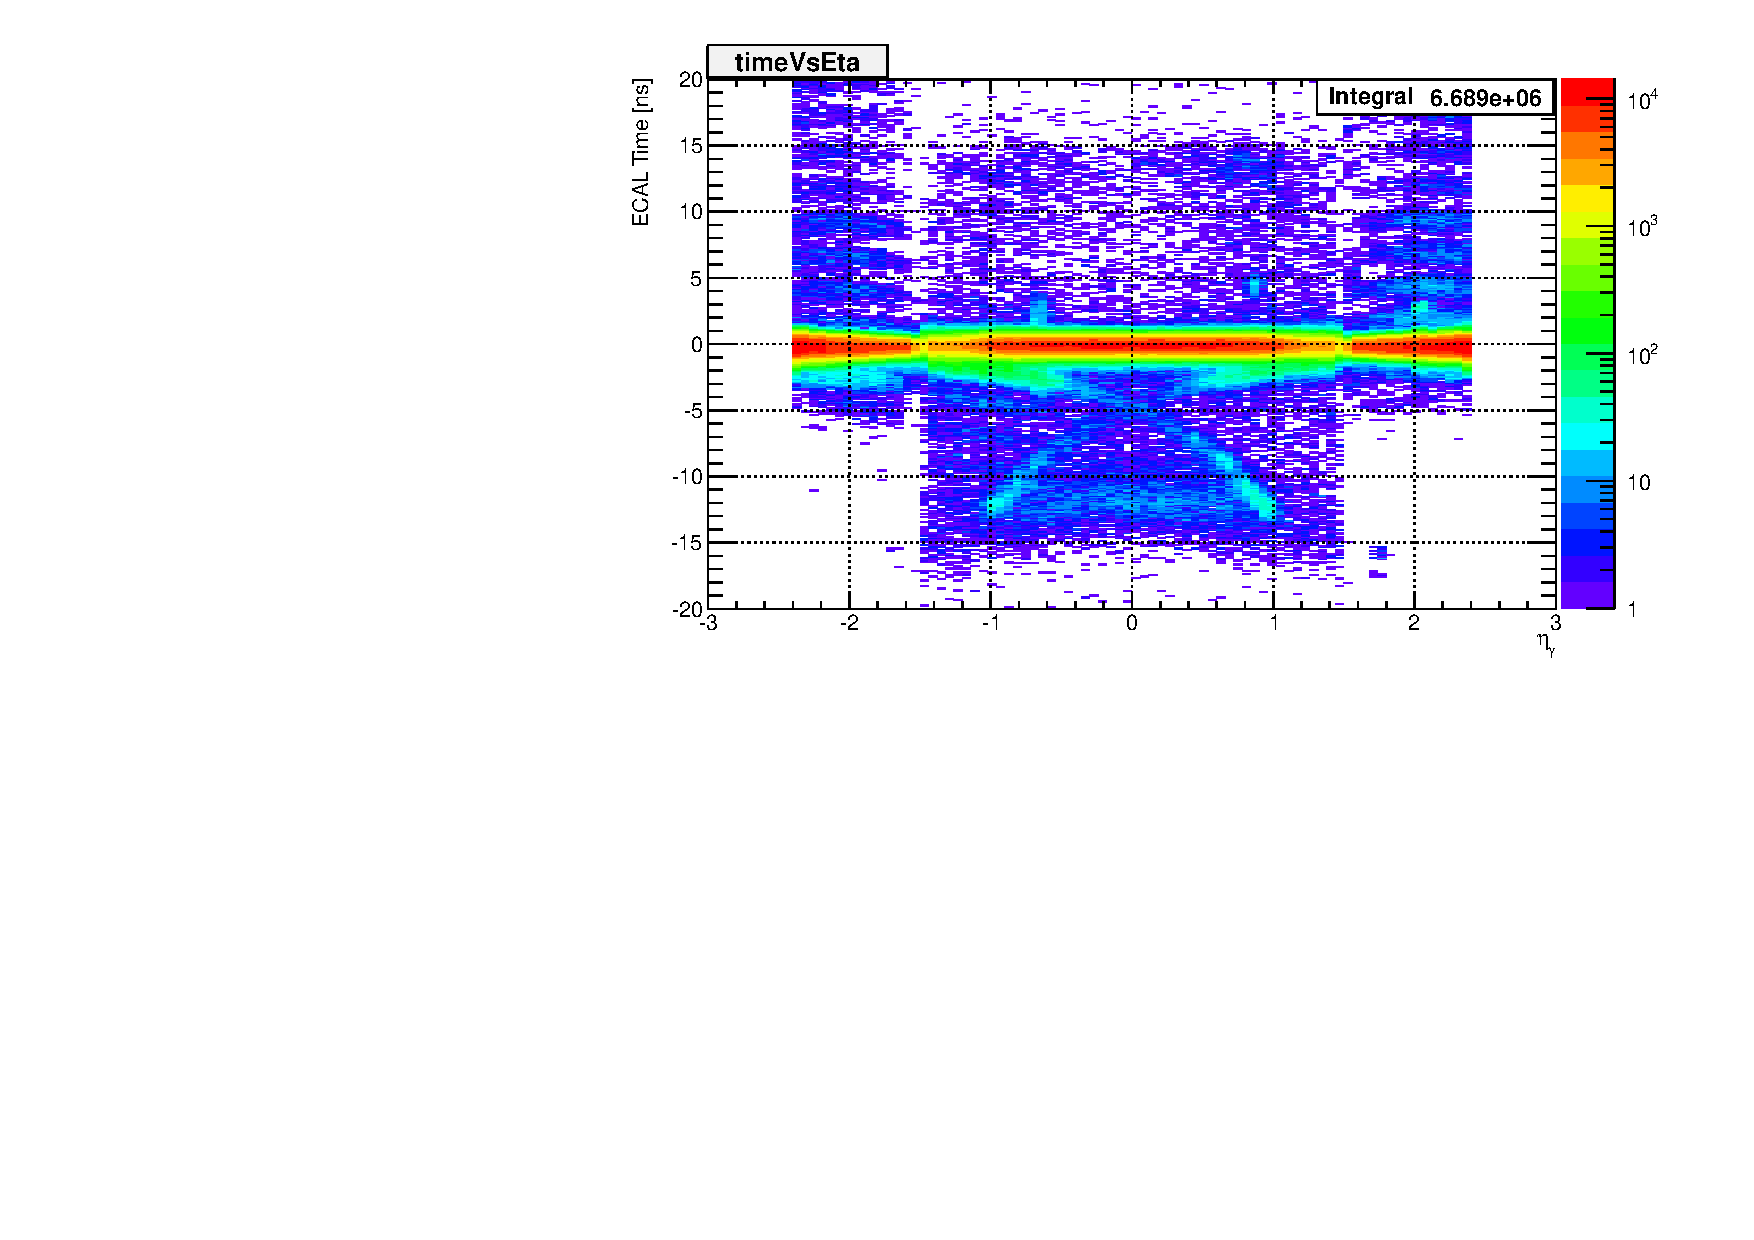
\includegraphics[height=6cm, width=0.5\textwidth]{THESISPLOTS/SinglePhotonDataSet-TimeVsEta.pdf}
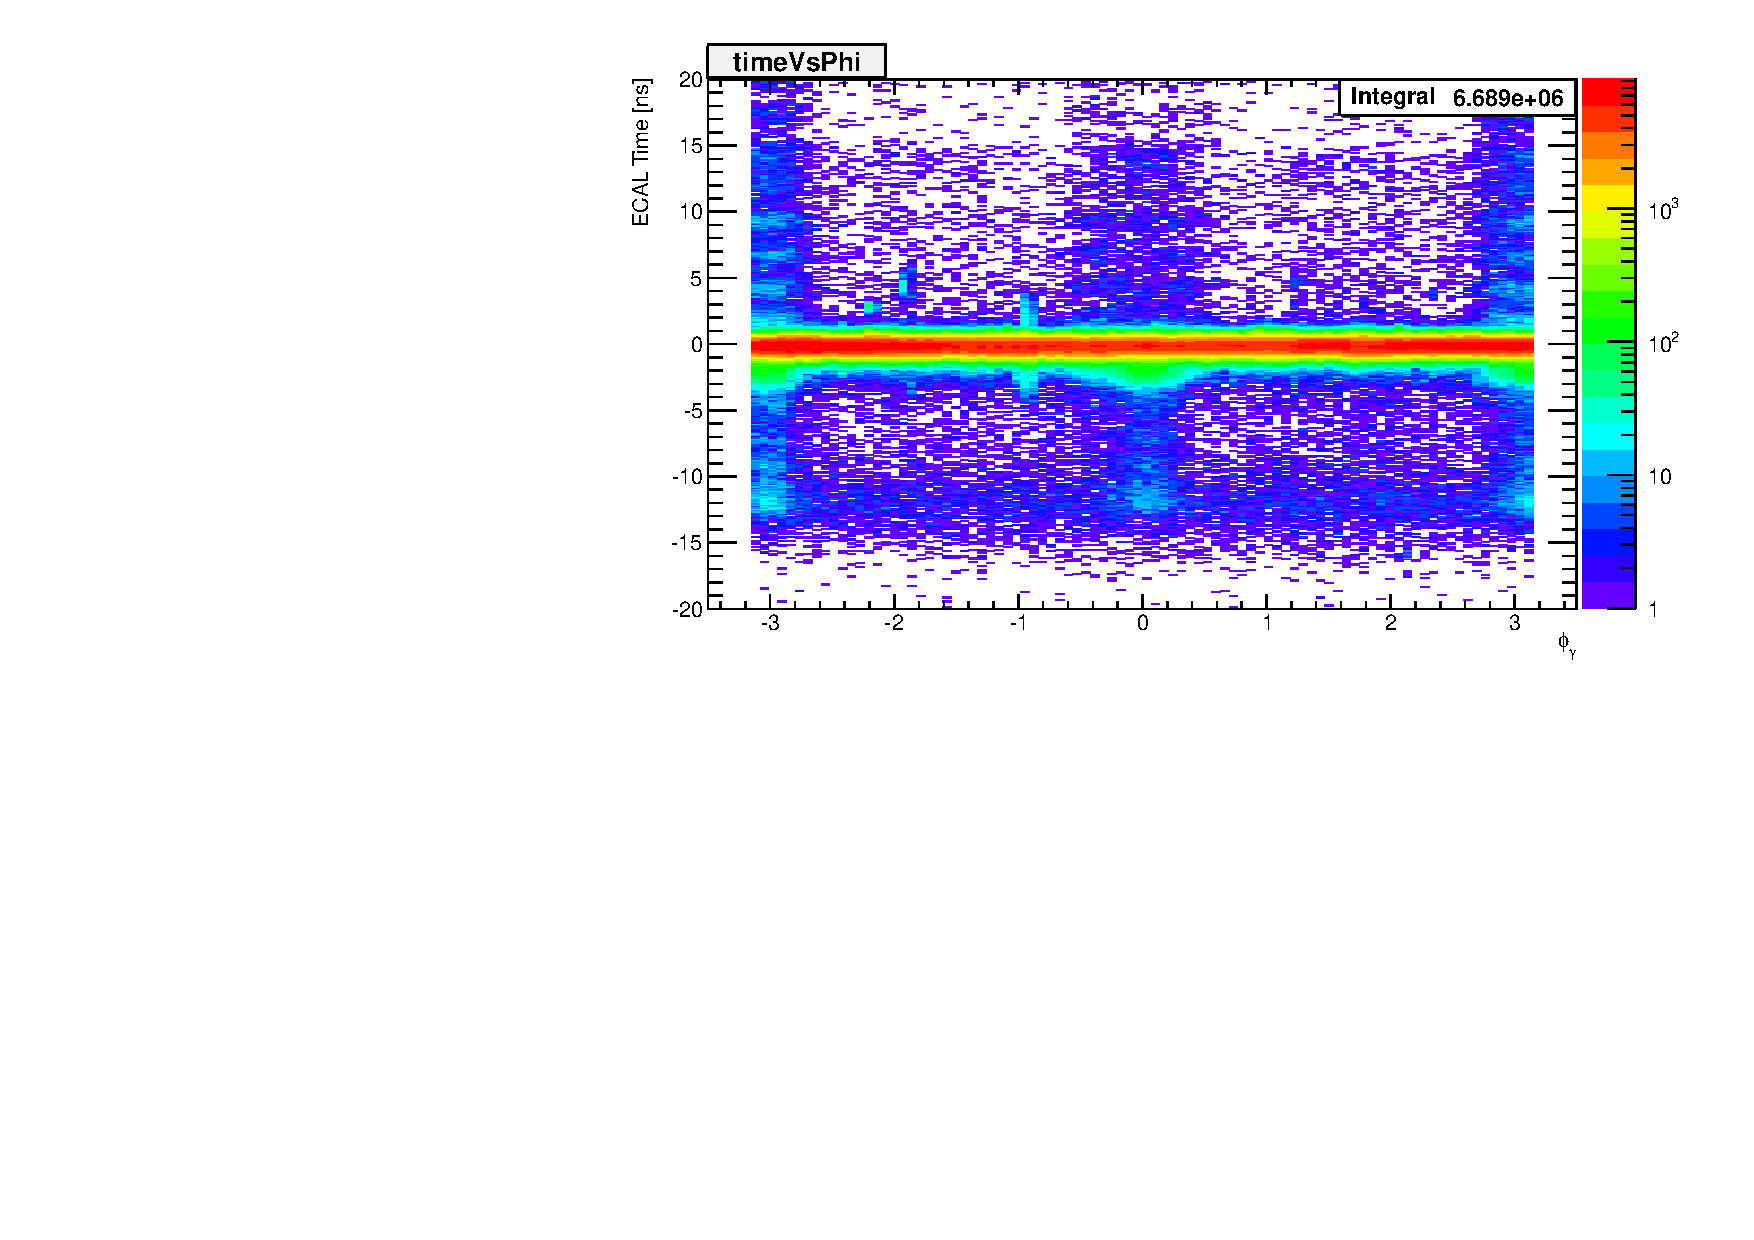
\includegraphics[height=6cm, width=0.5\textwidth]{THESISPLOTS/SinglePhotonDataSet-TimeVsPhi.pdf}}
\mbox{
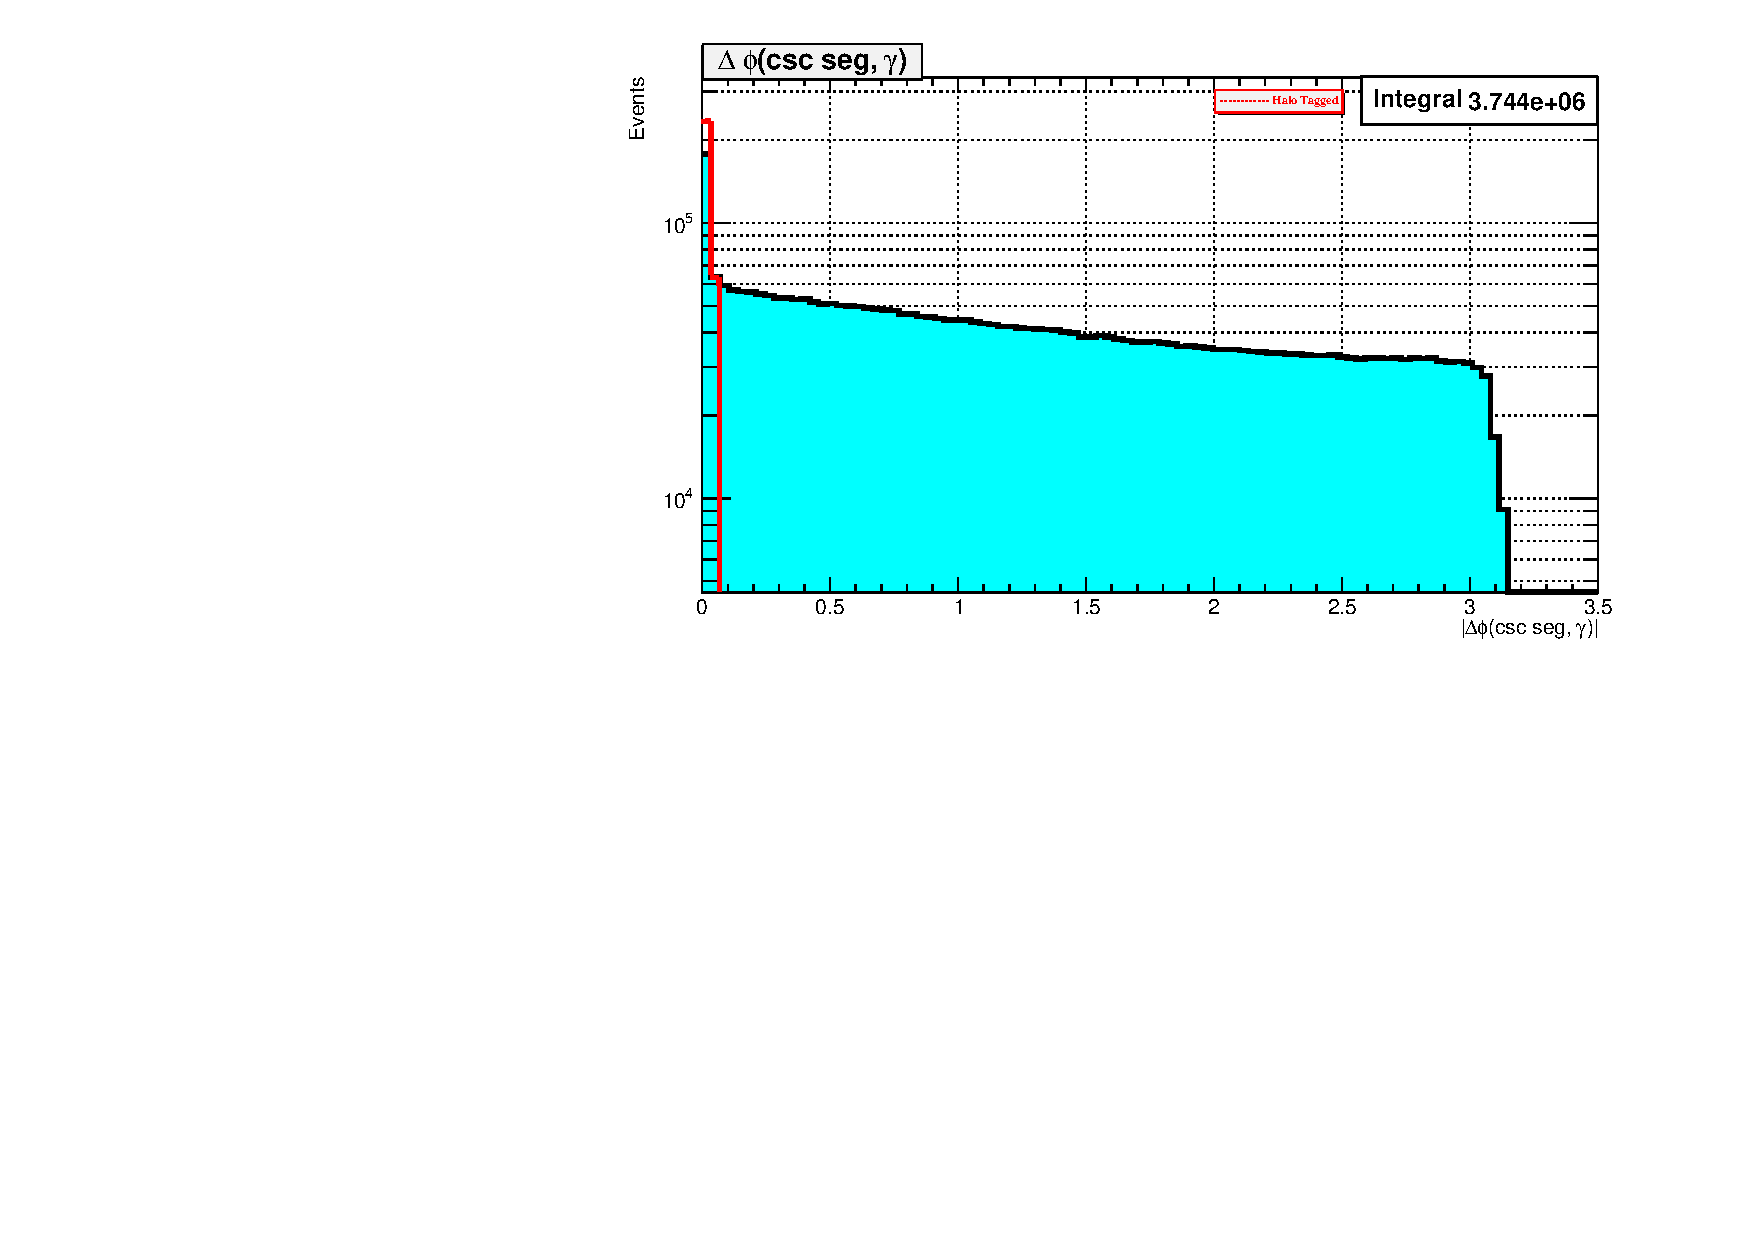
\includegraphics[height=6cm, width=0.5\textwidth]{THESISPLOTS/CSC-Segment-Halo-Tagging.pdf}
%{THESISPLOTS/CSC_Segment_Halo_data.png}
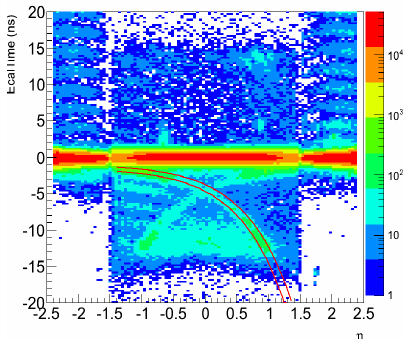
\includegraphics[height=6cm, width=0.5\textwidth]{THESISPLOTS/HALO-ECAL-TIME-Vs-ETA.png}}
\captionof{figure}{ECAL time Vs $\eta$~(left) and ECAL time Vs $\phi$~(right) and $CSC(Seg,\gamma)\Delta\phi$  for photons with $\pt > 80$~GeV from data. Halo photons show a clear matched between CSC segments and ECAL cluster in $\Delta\phi$  with their distribution peaking at $\phi = 0, \pm \pi$ and also the shape of their expected time.}
\label{fig:HALO}
\end{center} 



\subsubsection{Cosmic Photons}
Cosmic muons like beam Halo muons with sufficient energy  will also bremsstrahlung in the ECAL producing photons referred here as \textit{cosmic photons}. Unlike halo muons, cosmic muons can arrive at ECAL from any direction. Barrel cosmic photons  are expected to be produced from cosmic muons with hits in the Drift Tubes~(DT) segments. Using the DT hits and their corresponding  photon supercluster $\eta-\phi$ position in ECAL, we can match this  hit position in DT segments to ECAL photon superclusters within $\Delta\eta$ and $\Delta\phi$. The two dimensional distribution for $DT\Delta\eta(DT,\gamma)$ and $DT\Delta\phi(DT,\gamma)$ for this matching for events with photon time above, $t_{\gamma} > 2$~ns and time below, $t_{\gamma} < -3$~ns is shown in figure \ref{fig:COSMIC}. We conclude that events containing photons with small $\Delta\eta$ and $\Delta\phi$ to be candidate cosmic photons. Comparing this to $\Delta\eta$  and $\Delta\phi$ 2-dimensional distributions of photons from a pure cosmic muons sample~(data taken when no proton-proton collisions is happening) show these distributions to be very similar as seen in figure \ref{fig:COSMIC}.

\begin{center}
\centering
\mbox{
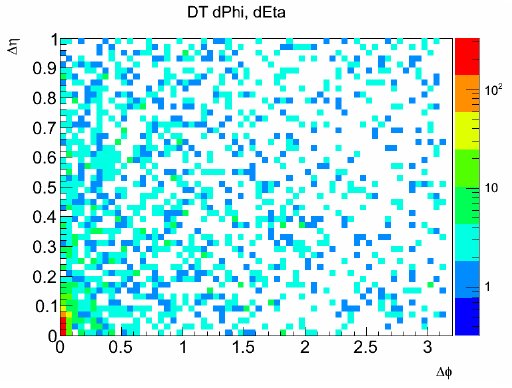
\includegraphics[height=6cm, width=0.5\textwidth]{THESISPLOTS/Cosmic_Ray_Photons_Data.png}
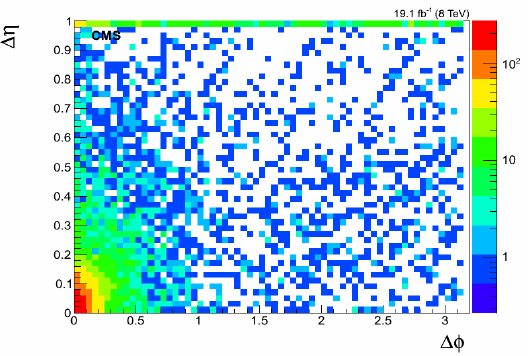
\includegraphics[height=6cm, width=0.5\textwidth]{THESISPLOTS/Cosmic_Ray_Photons_Cosmic_dataset.png} }
\captionof{figure}{2 dimensional plot showing $DT\Delta\eta(Seg,\gamma)$ against $DT\Delta\phi(Seg,\gamma)$ for photons with $\pt > 80$~GeV, ECAL Time, $ t_{\gamma} > 2$~ns and ECAL Time $t_{\gamma} < -3$~ns from proton-proton collision data~(left) and  pure cosmic muon data~(right). Small $\Delta\eta$ and $\Delta\phi$ are cosmic photon candidates.}
\label{fig:COSMIC}
\end{center}

\subsubsection{Anomalous Photons: Spikes}
Neutrons and some charge hadrons which deposit their energy directly to the APDs instead of the crystal scintillation are referred to as \textit{anomalous signal} or \textit{spikes}. Spikes can mimic the kinematics of true photons from proton-proton collisions  leading to the miss-identification of spikes as true photons. Spikes like true energetic photons can be isolated and so easily pass photon isolation cuts without being identified. A spike supercluster usually consists of very few crystals and most of the time single or double crystals except when embedded in a true photon of high electromagnetic fraction jets where they consist of may crystals and are difficult to identify. However, most spikes show a different signal pulse shape to that of true photons and also have large negative ECAL time especially at $t_{\gamma} \approx -12.0$~ns region. In addition to using energy topological selection cuts, which are based on the spike crystal energy deposits, during ECAL cleaning one can also use the $\chi^{2}$ fit value of the timing reconstruction to identify and reject spikes. Spike cleaning is performed during online and offline super cluster reconstruction. However, this online cleaning is not entire very efficient. Since ECAL clusters belonging to spikes are usually made up of very few crystals compared to photons clusters with many crystals, using the number of crystals in a reconstructed super cluster can be used to distinguish true isolated photons from events with spikes. It has been observed that spike contributions increases with increase in LHC luminosity. Thus, as a selection criteria, photons passing our cosmic photons and halo photons identification and with number of good crystals less than $7$ are considered to be spike candidates. Figure \ref{fig:SPIKES} show the distribution of the number crystals in a photon super cluster comparing photons with ECAL time, $ t_{\gamma} < 0$~ns, in-time photons~(ECAL $ -2.0 < t_{\gamma} < 0$~ns and  selected spike and halo control sample. The spike control sample is selected using the spike energy topological cut "\textit{swiss-cross}" variable in the region with $t_{\gamma} \approx -12.0$~ns where it is observed that spike concentration is high, is used to identify and reject events with spikes during super cluster reconstruction. We observe as shown in figure \ref{fig:SPIKES}(\textit{left}) that most spikes always have fewer($ < 7$) crystals is their photon supercluster.

\begin{center}
\centering
\mbox{
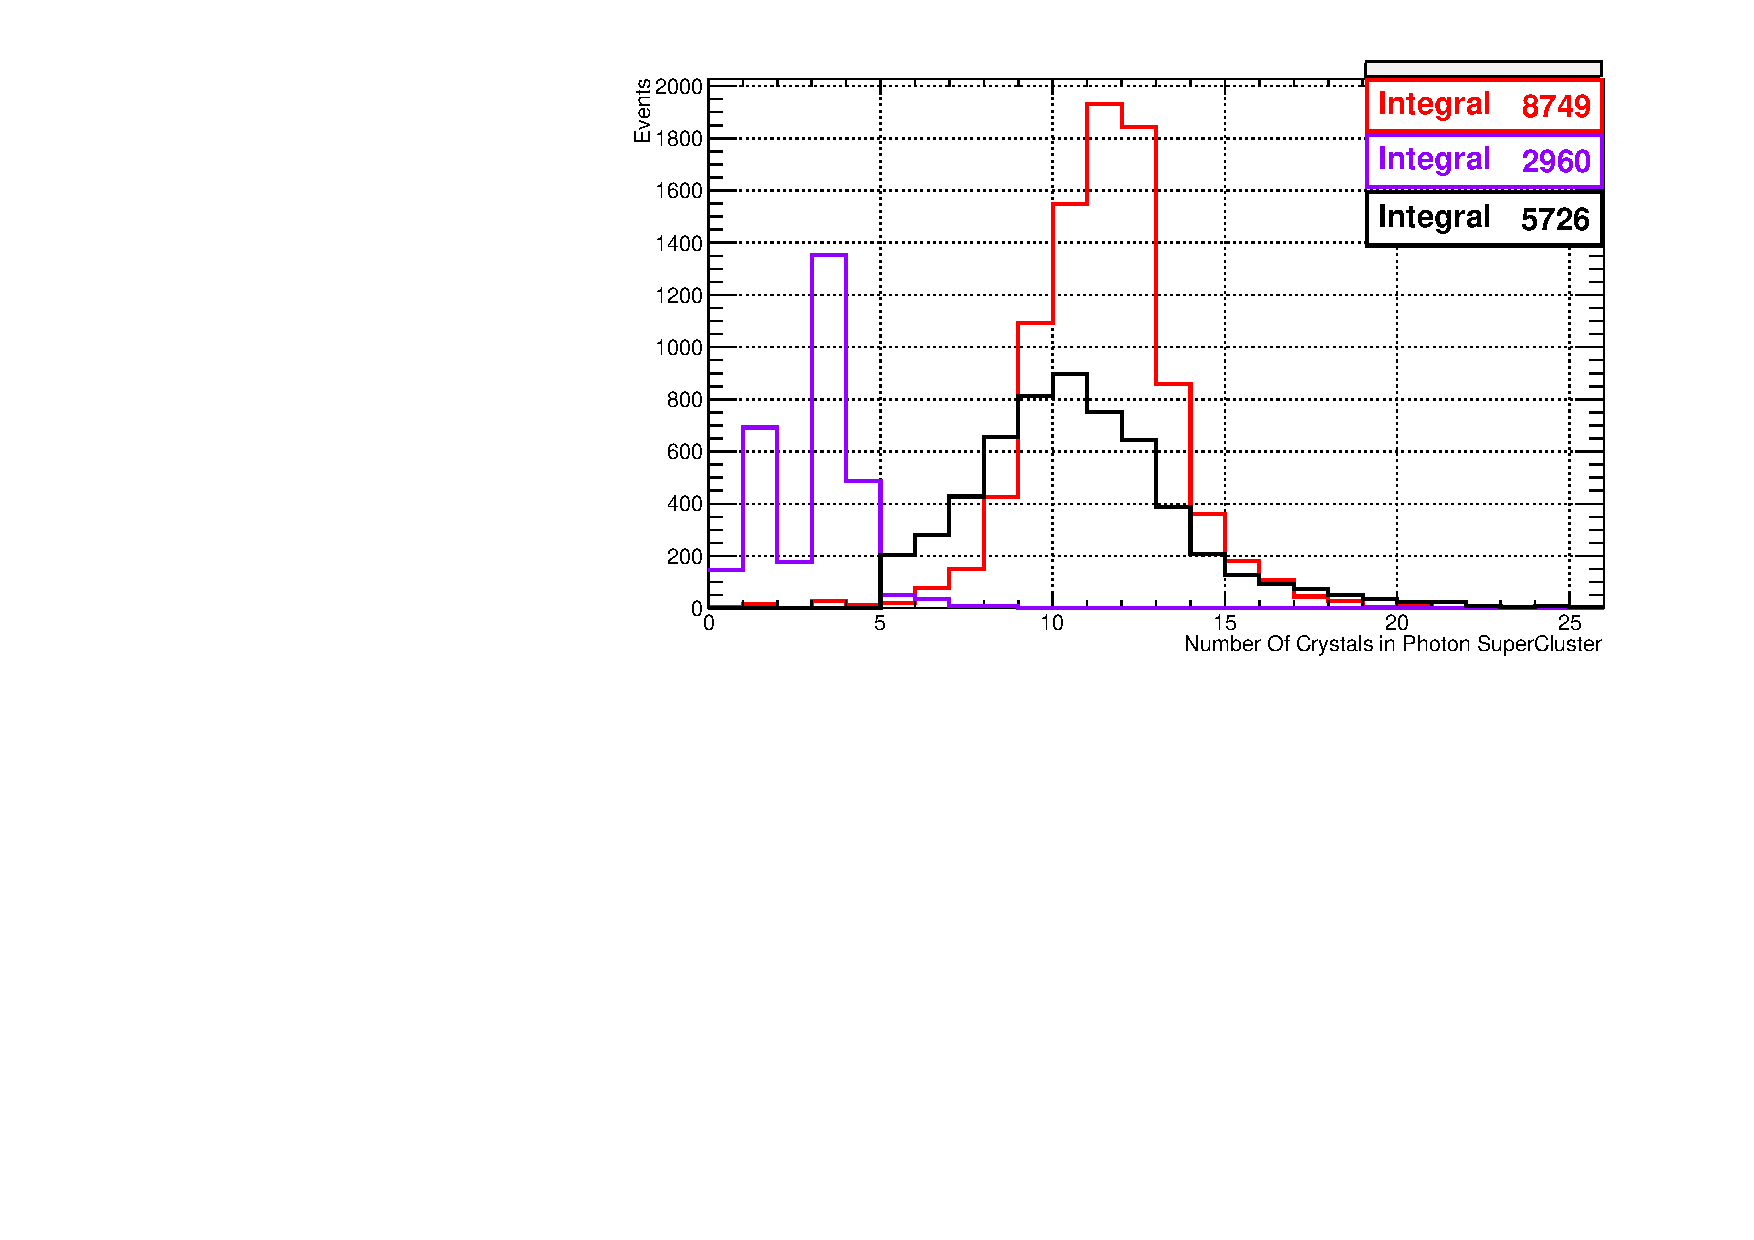
\includegraphics[height=7cm, width=0.5\textwidth]{THESISPLOTS/Number-Of-Crystals-In-Photon-SC.pdf}
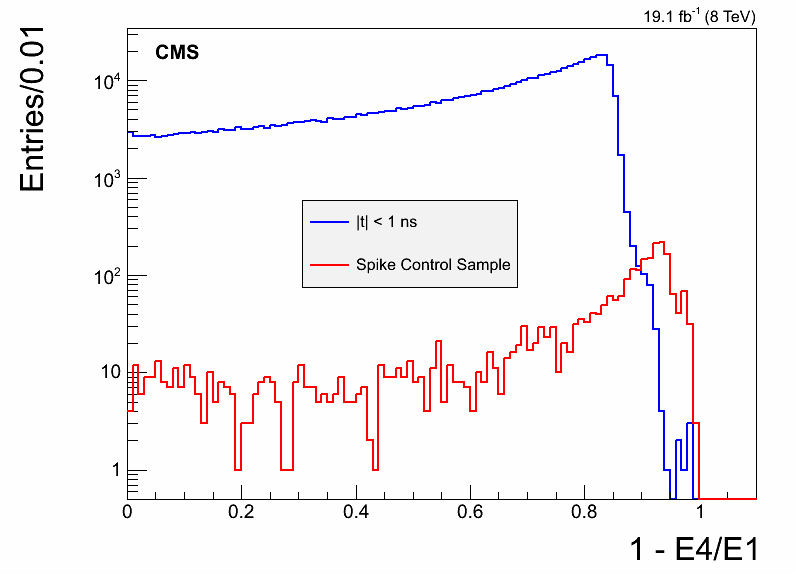
\includegraphics[height=7cm, width=0.5\textwidth]{THESISPLOTS/swissX.png} }
\captionof{figure}{Plot showing  \textit{number of crystals} in photon supercluster for photons from the region with ECAL Time, $t_{\gamma} < 0$~ns. Figure shows the timing distribution of candidate true photons(black), spike candidate photons~(magenta) and halo candidate photons~(red). The toplogical swiss-cross variable~($1- E_{4}/E_{1}$) distribution is shown comparing true photons~($|t_{\gamma}| < 1.0 $) to spike populated sample.}
\label{fig:SPIKES}
\end{center}


\subsection{Collision Backgrounds}

\subsubsection{QCD Photons and Pile Up}
%The LHC is designed to collide proton bunches every $25$~ns, but during the \texttt{2012 LHC} run, $50$~ns proton bunch collisions occurred. 
Collisions from the main proton bunches happening every $50$ns during \texttt{2012 LHC Run I} are not the only collisions that can occur at the LHC. The presence of  satellite/ghost bunches spaced in $5.0$~ns or $2.5$~ns discussed in section $3.1.5$ along LHC bunch structure can also collide producing delayed photons either from collisions between these satellite/ghost bunches or with the main proton bunch.
As observed in figure \ref{fig:TIMEECAL}, photons from these events are a serious background source to delayed photons and most of these photons will pass all the above event and photon selection criteria. Thus, it is imperative to 
estimate delayed photon contributions from satellite/ghost bunches is it is not negligible. Since these background source is non-reducible and the kinematics of these events are very similar, we employ the standard \texttt{ABCD} method to for estimating these background contribution to the signal region. However, we only perform this estimation after cleaning for possibly non-collision event contamination.



\subsection{Event Cleaning, Veto Performance and Fake Rate}
Using the derived kinematic variables for halo, cosmic and spike photons, we apply selection cuts on these variables for tagging and rejecting contributions from non-collision events. These cuts are applied in addition to our above event selections cuts to perform the following event cleaning:
\begin{itemize}
\item Veto 0-jet events as this sample is highly populated with beam halo events, 
\item Veto events with $CSC\Delta\phi(Seg,\gamma) < 0.05$,
\item Veto events with $\Delta\eta(DT Seg,\gamma) < 0.1$ and $\Delta\phi(DT Seg,\gamma) < 0.1$ .
\item Only photons with $|\eta_{\gamma}| < 1.45$ are considered,
\item Veto events with photons with Number of Good crystals $ < 7$ and $ 1-E_{4}/E_{1} > 0.98$.
\item Remove photons tagged as halo and cosmic photons,
\item Veto events with less than $2$-jets.
\end{itemize}
Events which pass all these additional selection criteria make up the sample which is used to estimated our final background to our signal.
Since it is very challenging to define pure control samples for each non-collision background source without possible contamination, we estimate the fake rates from the above veto or rejection conditions using in-time~($|t_{\gamma}| < 2.0$~ns) photon sample where we believe non-collision contribution is small compared to true photons from collision.
Our measured fake rates are shown in table \ref{tab:EVTC}.
\begin{center}
\centering
\begin{tabular}{|c| c|}
%\mbox{Fake Rate }
\hline
\bfseries{Background Source} & \bfseries {Fake Rate}(\%)\\
\hline\hline
\textit{Halo Photons} & ~$\approx 3$ \\
\textit{Cosmic Muons} & ~$\approx 1.4$ \\
\textit{Spikes} & $\approx 0.4$ \\
\hline
\end{tabular}
\captionof{table}{Fake rates for different non-collision cleaning.}
\label{tab:EVTC} 
\end{center}
After performing our event cleaning criteria, tagging and rejection of most of halo, cosmic and spike events, our residual background photon timing distribution is shown in figure \ref{fig:RESIDUAL} with the different sources of our background tags.
We now perform an \textsf{ABCD} background estimation technique on this residual background to estimate possible contamination of the remaining non-collision background to signal.

\begin{center}
\centering
\mbox{
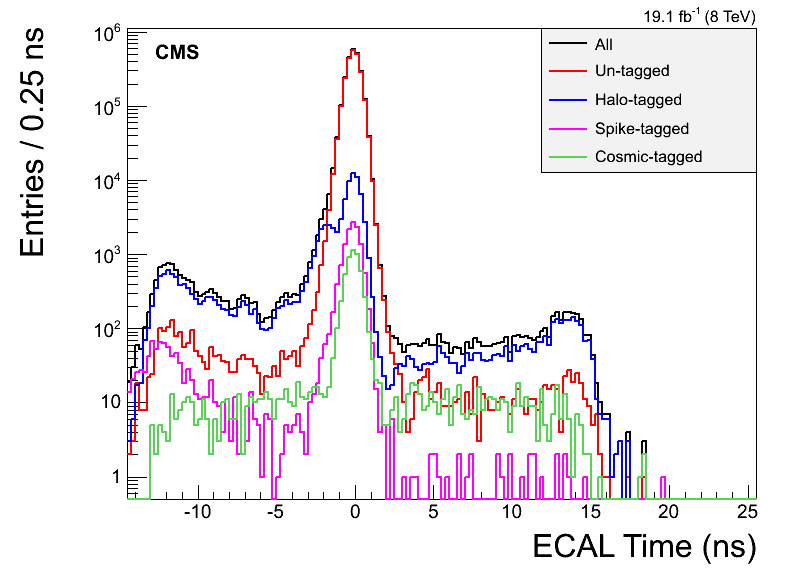
\includegraphics[height=8cm, width=0.8\textwidth]{THESISPLOTS/TimeForAll.png}
%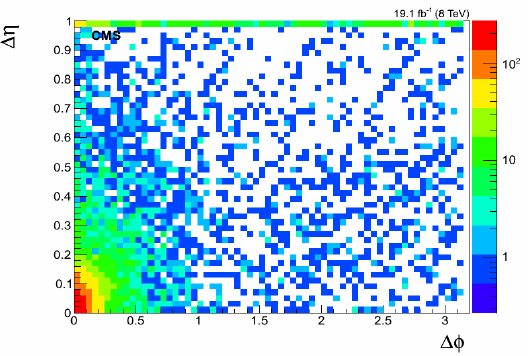
\includegraphics[height=6cm, width=0.5\textwidth]{THESISPLOTS/Cosmic_Ray_Photons_Cosmic_dataset.png} 
}
\captionof{figure}{Residual Background after tagging the different non-collision background sources using the methods described in text.}
\label{fig:RESIDUAL}
\end{center}



\subsubsection*{Residual Background Estimation Using ABDC Technique}
In order to estimating the background contribution from collision and non-collision sources, we employ a 3-dimensional space involving ${\ETslash}$~~, ${\ETslash}^{\gamma}$~~ and photon ECAL time, $t_{\gamma}$.  Our signal events are those with $3.0 < t_{\gamma} < 13.0$~ns with large \MET , and by large \MET , we mean events with ${\ETslash}^{\gamma} > 60$~GeV, ${\ETslash}$~~$ > 60$~GeV. Non-collision events as already seen can also have large time, since they are mostly out-of-time and by \MET calculation and corrections(see discussion above) should have large  ${\ETslash}^{\gamma}$~~ and small ${\ETslash}^{\gamma}$~~. Events from collision on the other hand are produced mostly in-time~($ -2.0 < t_{\gamma} < 2.0$~ns) except in cases of timing mis-measurements or ghost/satellite contributions where $t_{\gamma} > 3.0$~ns. Collision events, mostly produced through SM interactions, cannot be produced with large correctly calculated \MET, \eg $\gamma +$ jets events are produced with very small \MET, however due to timing mis-measurements, they may appear out-of-time and assigned large \MET. Thus we conclude that collision events will generally have small $\ETslash$~~ but large ${\ETslash}^{\gamma}$~~. 
 %But if the collision event is produced and arrives at ECAL with $t_{\gamma} > 3$~ns, and the \MET is not properly calculated (since events with photons ECAL time, $|t_{\gamma}| > 3$~ns are rejected during standard super cluster reconstruction with their \pt contribution  not taken into account in the \MET calculation) which in this case is large ${\ETslash}$~~, they will fluctuate or be easily considered as additional contribution to the non-collision background estimation in our signal region.
 
We select control samples~(CS) defined by ${\ETslash}$~~, ${\ETslash}^{\gamma}$~~ and $t_{\gamma}$ according to the \textsf{ABCD} technique to estimate our background contributions while remaining vigilant and taking into account the possible contamination to each background source from possible fluctuations in event rate as a result of our selection cuts in defining these CRs.
The overall estimation technique is verified through a closure test procedure and the collision background estimation is validated using an extra control sample of $Z \rightarrow \EE$ events for $Z$ candidates reconstructed from photon candidates extended to include out-of-time events.
\begin{enumerate}
\item $\mathbf{{\ETslash}^{\gamma}}$~~$ > 60$~\textbf{GeV}: CS in which collision~(QCD) background is suppressed while halo, cosmic ray and spike photon is enhanced since most non-collision background photons are produced with high \pt hence large ${\ETslash}^{\gamma}$~~.
Using this CS, we define four regions for estimating the non-collision background contribution using the \textsf{ABCD} recipe.
\begin{center}
\centering
\begin{tabular}{||c| c| c||}
\hline \hline

\bfseries{Non-Collision} & \bfseries{${\ETslash}$~~$ < 60$~GeV} &  \bfseries{${\ETslash}$~~$ > 60$~GeV}\\
      
\hline \hline
$3.0 < t_{\gamma} < 13.0$~ns. &  \textsf{$C$} &  \textsf{$D$} \\
\hline
$ -10.0 < t_{\gamma} < -3.0$~ns & \textsf{$A$} &  \textsf{$B$} \\
\hline\hline 
\end{tabular}
\captionof{table}{\textsf{ABCD} Control Regions~(CRs) for estimating non-collision background.}
\label{tab:NON-COLLISION} 
\end{center}

%\begin{itemize}
%\item \textbf{A}: Events with ${\ETslash}$~~$ < 60$~GeV and $ -10.0 < t_{\gamma} < -3.0$~ns.
%\item \textbf{C}: Events with ${\ETslash}$~~$ < 60$~GeV and $3.0 < t_{\gamma} < 13.0$~ns.
%\item \textbf{B}: events with ${\ETslash}$~~$ > 60$~GeV and $-10.0 < t_{\gamma} < -3.0$~ns.
%\item \textbf{D}: events with ${\ETslash}$~~$ > 60$~GeV and $3.0 < t_{\gamma} <  13.0$~ns.
%\end{itemize}

Thus, the number of events expected in Control Region~(CR) \textbf{$D$} using table \ref{tab:NON-COLLISION} with the assumption that $\frac{N_{D}}{N_{B}} = \frac{N_{C}}{N_{A}}$  is given as:

\begin{equation}
N_{D} = \left(\frac{N_{B}}{N_{A}} \right)\cdot N_{C}
\end{equation}

\item $\mathbf{\ETslash}$~~$ > 60$~\textbf{GeV}: CS where non-collision background~(halo, cosmic and spike photons) contribution is suppressed while collision~(QCD) background contribution is enhanced.
Further dividing this CS and applying \textsf{$A^{\prime}$ $B^{\prime}$ $C^{\prime}$  $D^{\prime}$} method to estimated collision contribution is shown in table \ref{tab:COLLISION}.

\begin{center}
\centering
\begin{tabular}{||c| c| c||}
\hline \hline

\bfseries{Collision}       & \bfseries{${\ETslash}^{\gamma} < 60$~GeV} &  \bfseries{${\ETslash}^{\gamma} > 60$~GeV}\\
      
\hline \hline
$3.0 < t_{\gamma} < 13.0$~ns. &  \textsf{$C^{\prime}$} &  \textsf{$D^{\prime}$} \\
\hline
$ -2.0 < t_{\gamma} < 2.0$~ns & \textsf{$I^{\prime}$} &  \textsf{$I$} \\
\hline 
$ -10.0 < t_{\gamma} < -3.0$~ns & \textsf{$A^{\prime}$} &  \textsf{$B^{\prime}$} \\
\hline\hline 
\end{tabular}
\captionof{table}{\textsf{$A^{\prime}$ $B^{\prime}$ $C^{\prime}$ $D^{\prime}$} and \textsf{$I$ $I^{\prime}$} CRs for estimating collision background.}
\label{tab:COLLISION} 
\end{center}

\end{enumerate}
%\begin{itemize}
%\item $\mathbf{A^{\prime}}$: Events with ${\ETslash}^{\gamma} < 60$~GeV and $-10.0 < t_{\gamma} < -3.0$~ns.
%\item $\mathbf{B^{\prime}}$: Events with ${\ETslash}^{\gamma} > 60$~GeV and $-10.0 < t_{\gamma} < -3.0$~ns.
%\item $\mathbf{I^{\prime}}$: Events with ${\ETslash}^{\gamma} < 60$~GeV and $|t_{\gamma}| < 2.0$~ns.
%\item $\mathbf{I}$: Events with ${\ETslash}^{\gamma} > 60$~GeV and $|t_{\gamma}| < 2.0$~ns.
%\end{itemize}
%we also define a in time CR as:
%\begin{itemize}
%\item $\mathbf{C^{\prime}}$: Events with ${\ETslash}^{\gamma} < 60$~GeV and $ 3.0 < t_{\gamma} <  13.0$~ns.
% \item $\mathbf{D^{\prime}}$: Events with ${\ETslash}^{\gamma} > 60$~GeV and $3.0 < t_{\gamma} <  13.0$~ns.
% \item $\mathbf{I^{\prime}}$: Events with ${\ETslash}^{\gamma} < 60$~GeV and $|t_{\gamma}| < 2.0$~ns.
%\item $\mathbf{I}$: Events with ${\ETslash}^{\gamma} > 60$~GeV and $|t_{\gamma}| < 2.0$~ns.
%\end{itemize}

Using CRs defined in table \ref{tab:COLLISION}, we can estimate the contributions of collision background in both CRs $B$ and $D$ of our non-collision background CS as follows:
\begin{equation}
\displaystyle{N_{B}^{col} = N_{B^{\prime}}  = \left( \frac{I}{I^{\prime}} \right)\cdot N_{A^{\prime}}}, \quad \quad
\displaystyle{N_{D}^{col} = N_{D^{\prime}}  = \left( \frac{I}{I^{\prime}} \right)\cdot N_{C^{\prime}}}
\end{equation}
where we have assumed that $\frac{N_{B^{\prime}}}{N_{A^{\prime}}}  = \frac{N_{I}}{N_{I^{\prime}}}$ and  $\frac{N_{D^{\prime}}}{N_{C^{\prime}}}  = \frac{N_{I}}{N_{I^{\prime}}}$.
\newline

$N_{B}^{col}$ and $N_{D}^{col}$ are collision contributions to  CRs $B$ and $A$. The  final combined background estimation is given by equation \ref{eq:FBKG}.

\begin{equation}{\label{eq:FBKG}}
N_{D}^{Total} = \left(\frac{N_{B} - N_{B}^{col} }{N_{A}} \right)\cdot N_{C} + N_{D}^{col} 
\end{equation}
where $N_{D}^{Total} = N_{D}^{non-col} + N_{D}^{col}$ is the total background estimation in  our signal region.
%\begin{center}
%\centering
%\mbox{
%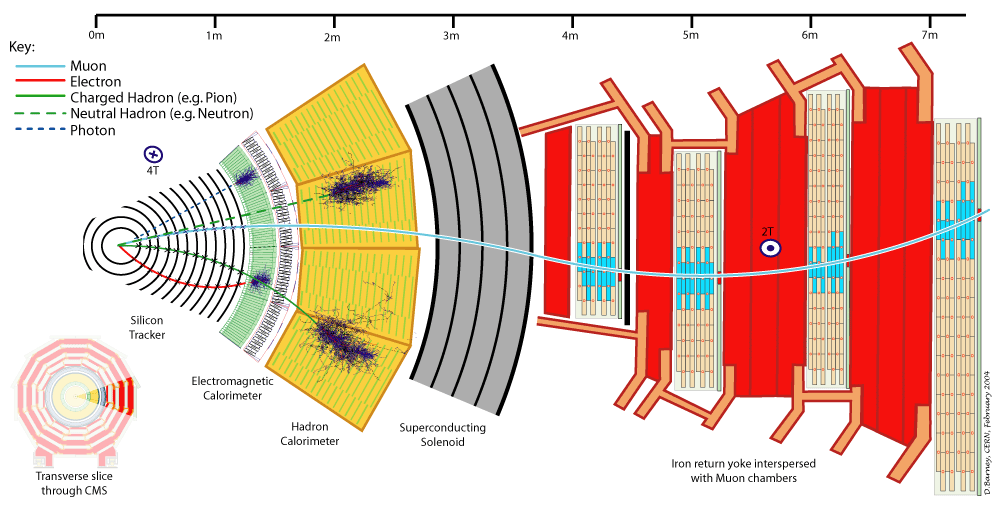
\includegraphics[scale=0.2]{THESISPLOTS/CMS_Slice.png}
%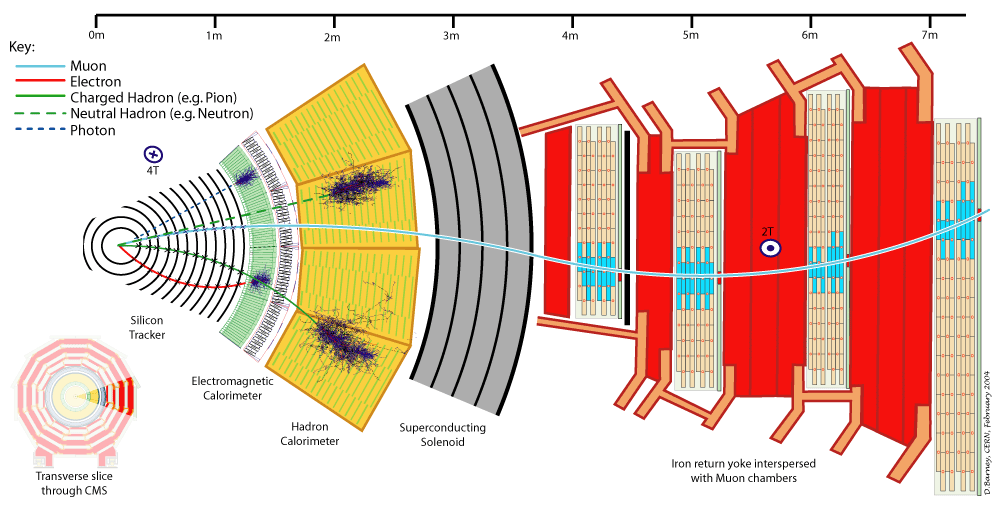
\includegraphics[scale=0.2]{THESISPLOTS/CMS_Slice.png}
%\captionof{figure}{Diagrams showing background estimation technique.}
%\label{fig:BKGESTI}
%\end{center}



\paragraph*{Closure Test}\mbox{}\\
Selecting events with $0$-jets and $1$-jet,  we performed closure test of our background estimation method. We also perform a cross-check on the assumptions used in our background estimations for small contributions for collision background using $Z\rightarrow \EE$ events. 
Our underlying assumption here is that background contributions to large timing from collision source referred here as QCD is very small and must be of the order of $10^{-5}$ in comparison to in-time photons. i.e the ratio 
$ N_{t_{\gamma} > 3~ns}/ N_{|t_{\gamma}| < 2.0~ns} \approx 10^{-5}$ with $N$ being the number of photons.
 The closure test compares the number of events observed in CR \textsf{$D$} to the number  expected using our \textsf{ABCD} background estimation method in the same CR \textsf{$D$}.
 We observed $10$ events while from using equation \ref{eq:FBKG}, we expected $16.78^{+2.95}_{-3.45}$. We argue that within our statistical uncertainties, there is quite an agreement between our expectation and observed events. The complete result from our closure test is shown in table \ref{tab:EVTC}. This gives us confidence that our  background estimation method is robust and reliable. We apply the same \textsf{ABCD} to estimate the background contribution in our signal sample. Our signal sample consist of events with at least $2$-jets, at least a single photon and ${\ETslash}^{\gamma} > 60$~GeV, ${\ETslash}$~~$ > 60$~GeV..

\begin{center}
\centering
\begin{tabular}{|c| c| c|}
%\mbox{Fake Rate }
\hline
\bfseries{Non-Collision} & \bfseries{ ${\ETslash}^{\gamma}$~~$ < 60$~\GeV} & \bfseries {${\ETslash}^{\gamma}$~~$ > 60$~\GeV} \\
\hline
 $3.0 < t_{\gamma} < 13.0$~ns & \textsf{C}($405$) & ~\textsf{D}($10$) \textcolor{blue}{16.78} \\
 $-10.0 < t_{\gamma} < -3.0$~ns & \textsf{A}($871$) & ~\textsf{B}($36$) \\
\hline \hline

\bfseries{Collision} & \bfseries{ ${\ETslash}$~~$ < 60$~\GeV} & \bfseries {${\ETslash}$~~$ > 60$~\GeV} \\
\hline 
 $3.0 < t_{\gamma} < 13.0$~ns & \textsf{$D^{\prime}$}($4$) & ~\textsf{D}($10$) \\
 $-2.0 < t_{\gamma} < 2.0$~ns & \textsf{$F^{\prime}$}($1353685$) & ~\textsf{F}($34543$) \\
 $-10.0 < t_{\gamma} < -3.0$~ns & \textsf{$B^{\prime}$}($5$) & ~\textsf{B}($36$) \\
\hline\hline 
\end{tabular}
\captionof{table}{Result from closure test of background estimation technique using $0$ and $1$-jet events. Numbers in bracket represent our expected background estimate using \textsf{ABCD} method.}
\label{tab:EVTC} 
\end{center}

\subsection{Background Estimation Cross Check}
The main assumption in our background estimation technique is that, the contribution from collision background events to out-of-time regions~($3.0 < t_{\gamma} < 13.0$~ns) is negligible.
In order to show that this assumption is correct, we select $Z\rightarrow \EE$ events from \texttt{SingleElectron} and \texttt{DoubleElectron} data sets of 2012. Our motivation is to use a control sample where contributions from non-collision events is very small.
We select $Z$ candidate events from an extended photon sample including out-of-time photon events according to the following selection criteria:
\begin{itemize}
\item The candidate two electrons for the $Z$ bosons must have individual $\pt > 25$~GeV,
\item The di-mass of these two electrons, $|m_{\EE} - 91| > 61$~$GeV/c^{2}$,
\item Each electron must be in the barrel, $|\eta_{e^{-}}| < 1.479$ and $ |\eta_{e^{+}}| < 1.479$.
\end{itemize}
 At the electron super cluster level,  we used the seed crystal time adjusted to account for the electron time of flight, as the electron time. The seed crystal must satisfy the recommended crystals or rechit cleaning criteria by the ECAL group which include \texttt{kWeird}, \texttt{kBad}, \texttt{kPoorCalib} used for rejecting crystals showing anomalous behavior like spikes, noisy, bad crystals or poorly calibrated crystals.
In this cross-check, we define our signal region as $Z$-candidate events with a well defined mass from both electrons i.e  $76 < |m_{\EE}| < 100$~$GeV/c^{2}$ while the non $Z$ events control sample are events which do not fall into this signal category.
A quick look at photon $t_{\gamma}$ vs $\eta_{\gamma}$ and $\phi_{\gamma}$ plots as previously shown for halo photons in figure \ref{fig:HALO}, shows that the electron candidates from the \texttt{Single/DoubleElectron} dataset when compared to the \texttt{SinglePhoton} dataset in figure \ref{fig:Elec} show no or very little contribution from cosmic, halo and anomalous photon events. This confirms our choice of the $Z$ candidate events sample as a reliable sample to study collision events as it is free from non-collision events.
\begin{center}
\centering
\mbox{
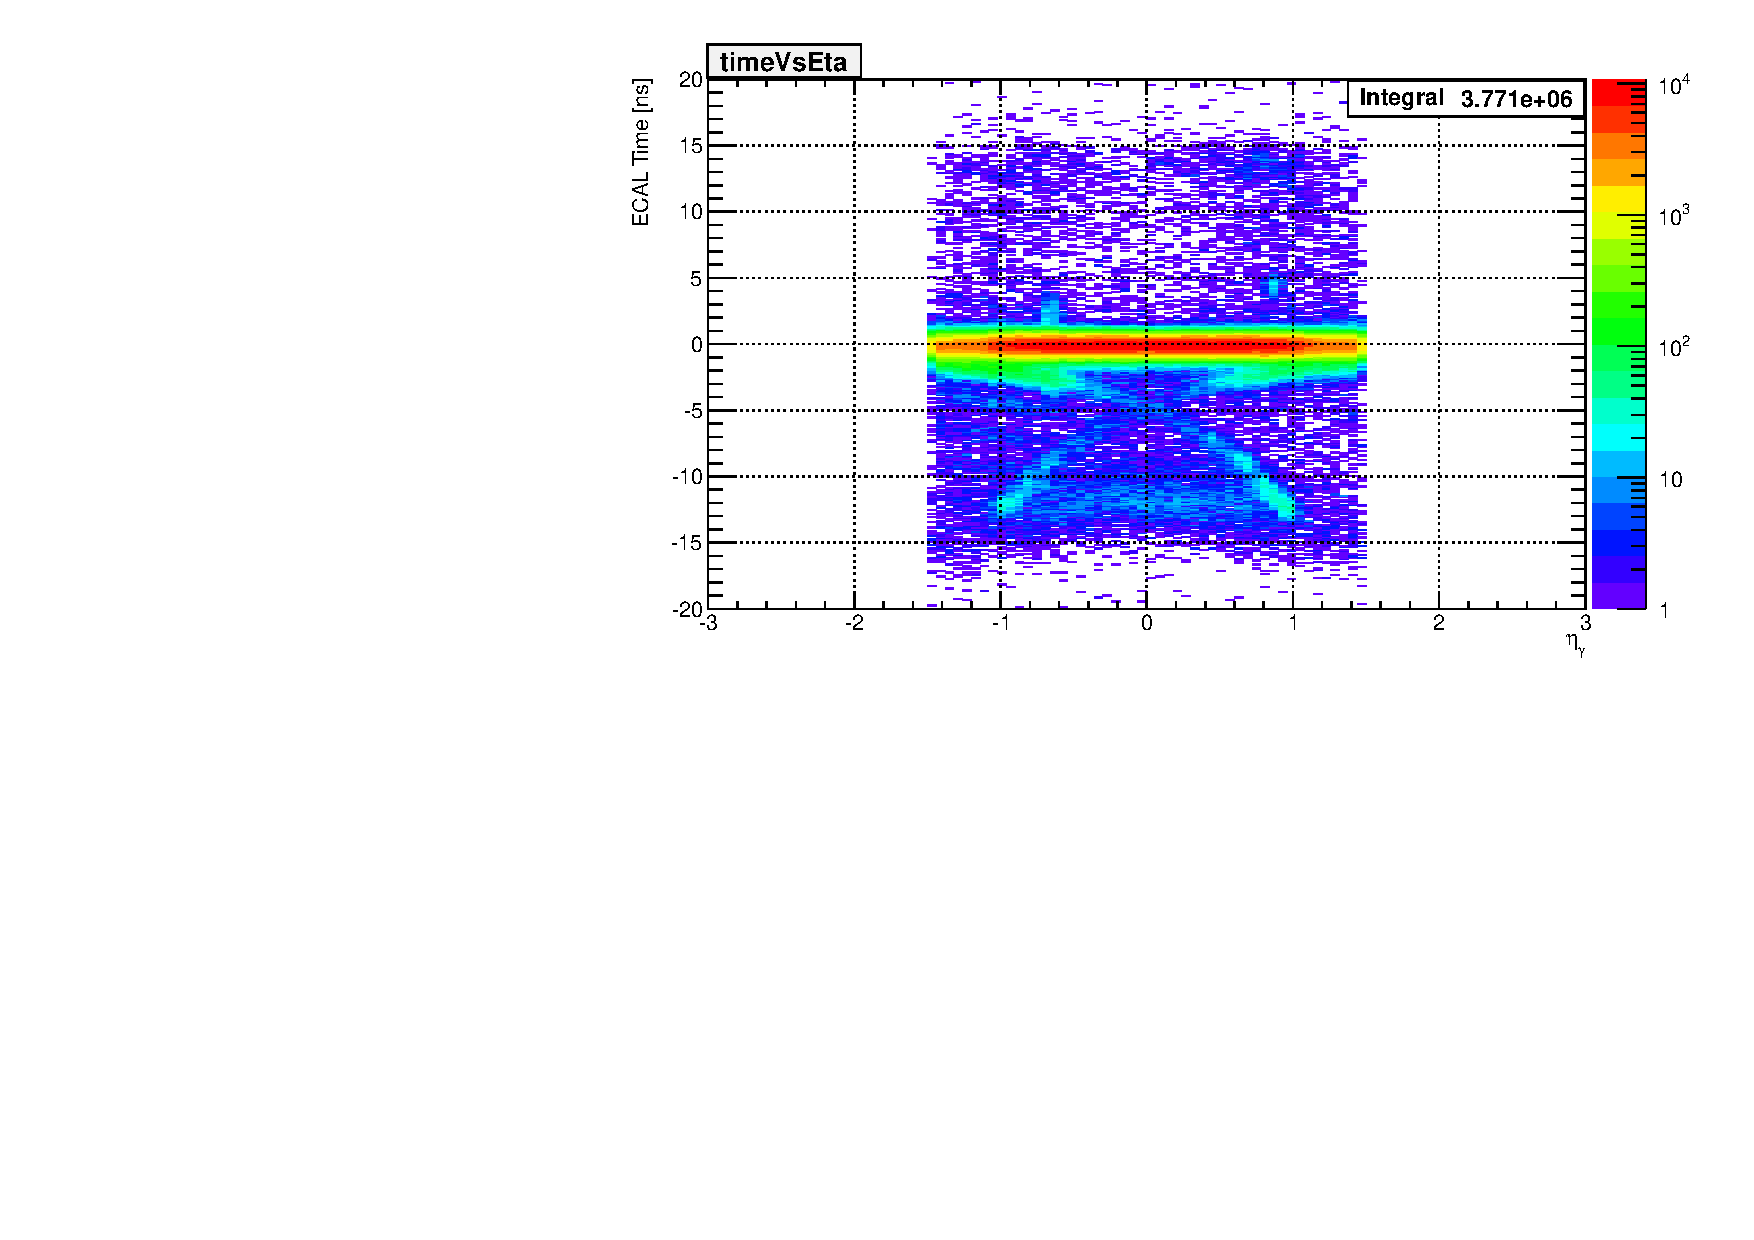
\includegraphics[height=6cm, width=0.5\textwidth]{THESISPLOTS/SinglePhotonDataSet-TimeVsEtaEB.pdf}
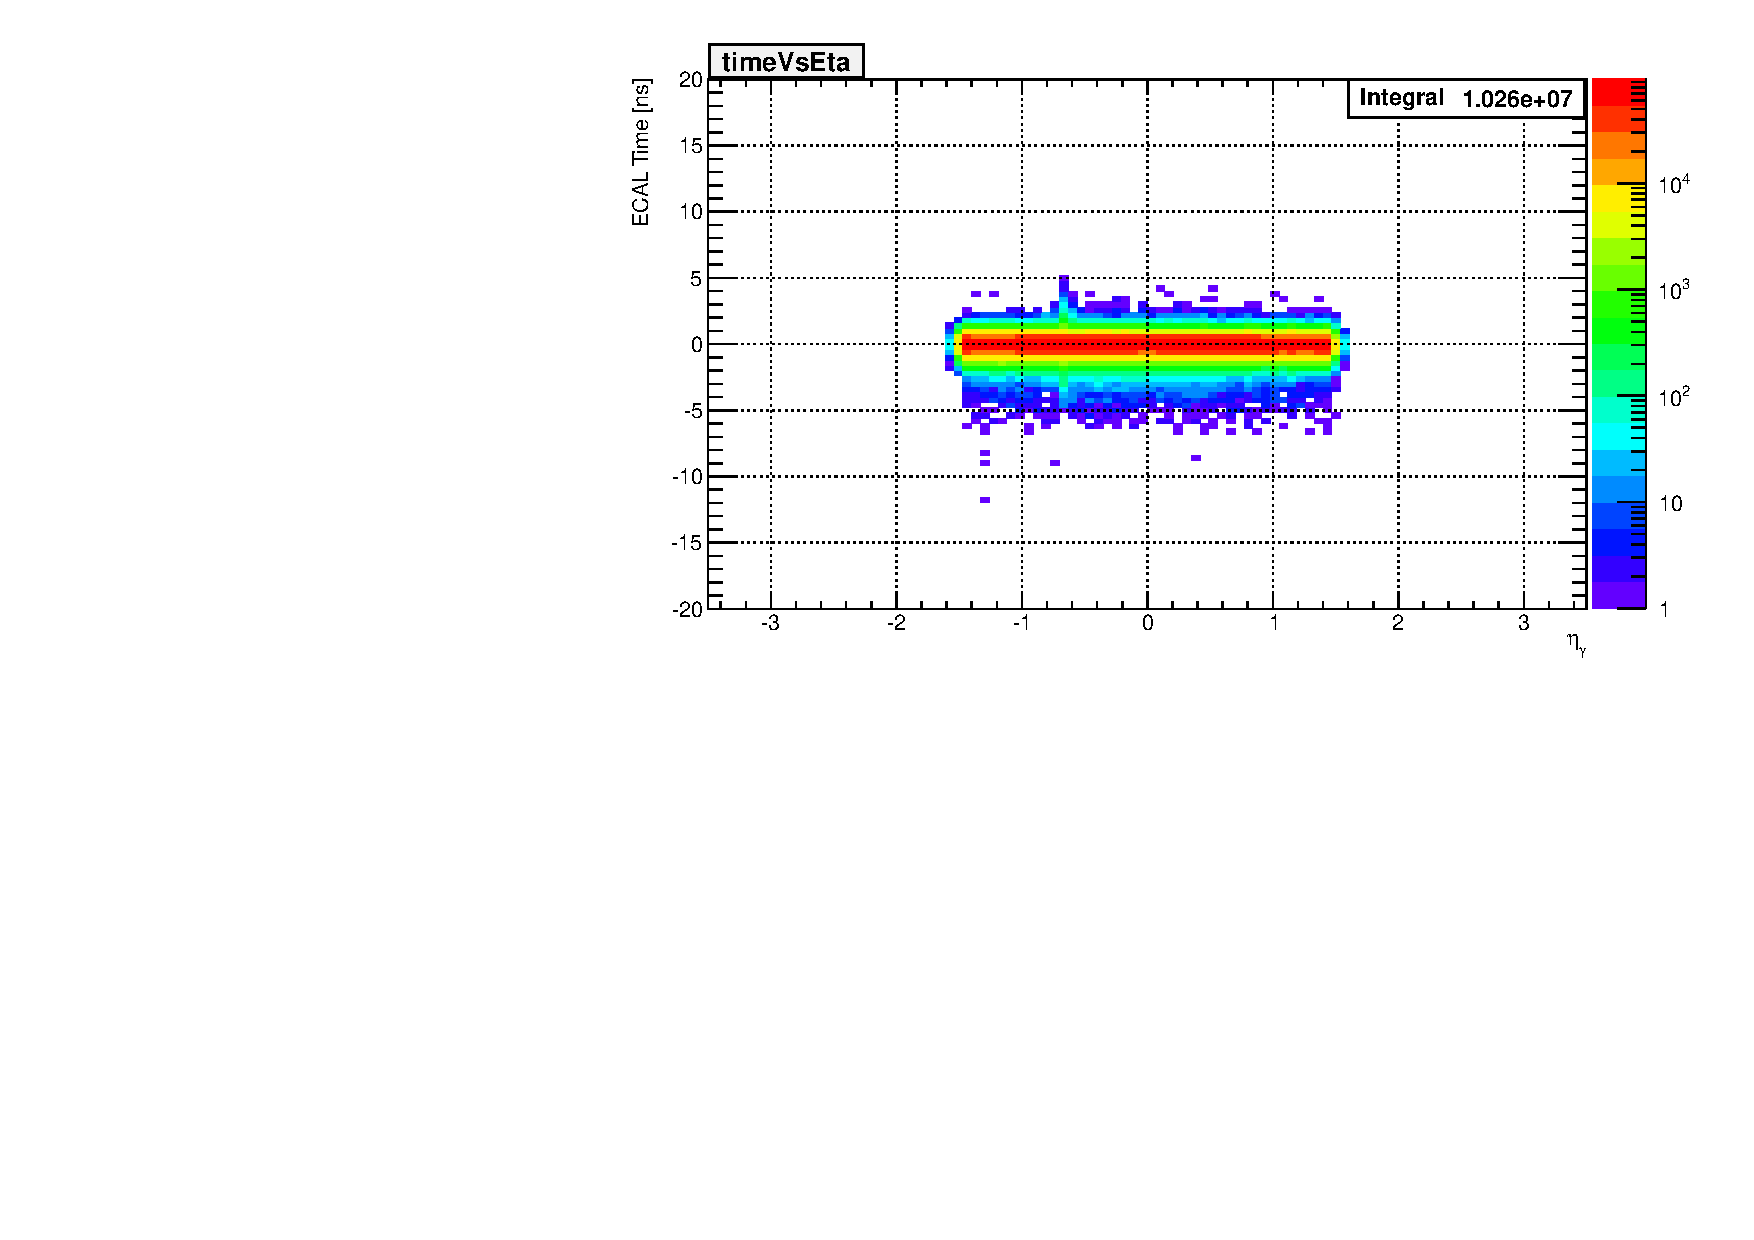
\includegraphics[height=6cm, width=0.5\textwidth]
{THESISPLOTS/ZCandidates_TimeVsEta.pdf}}
\mbox{
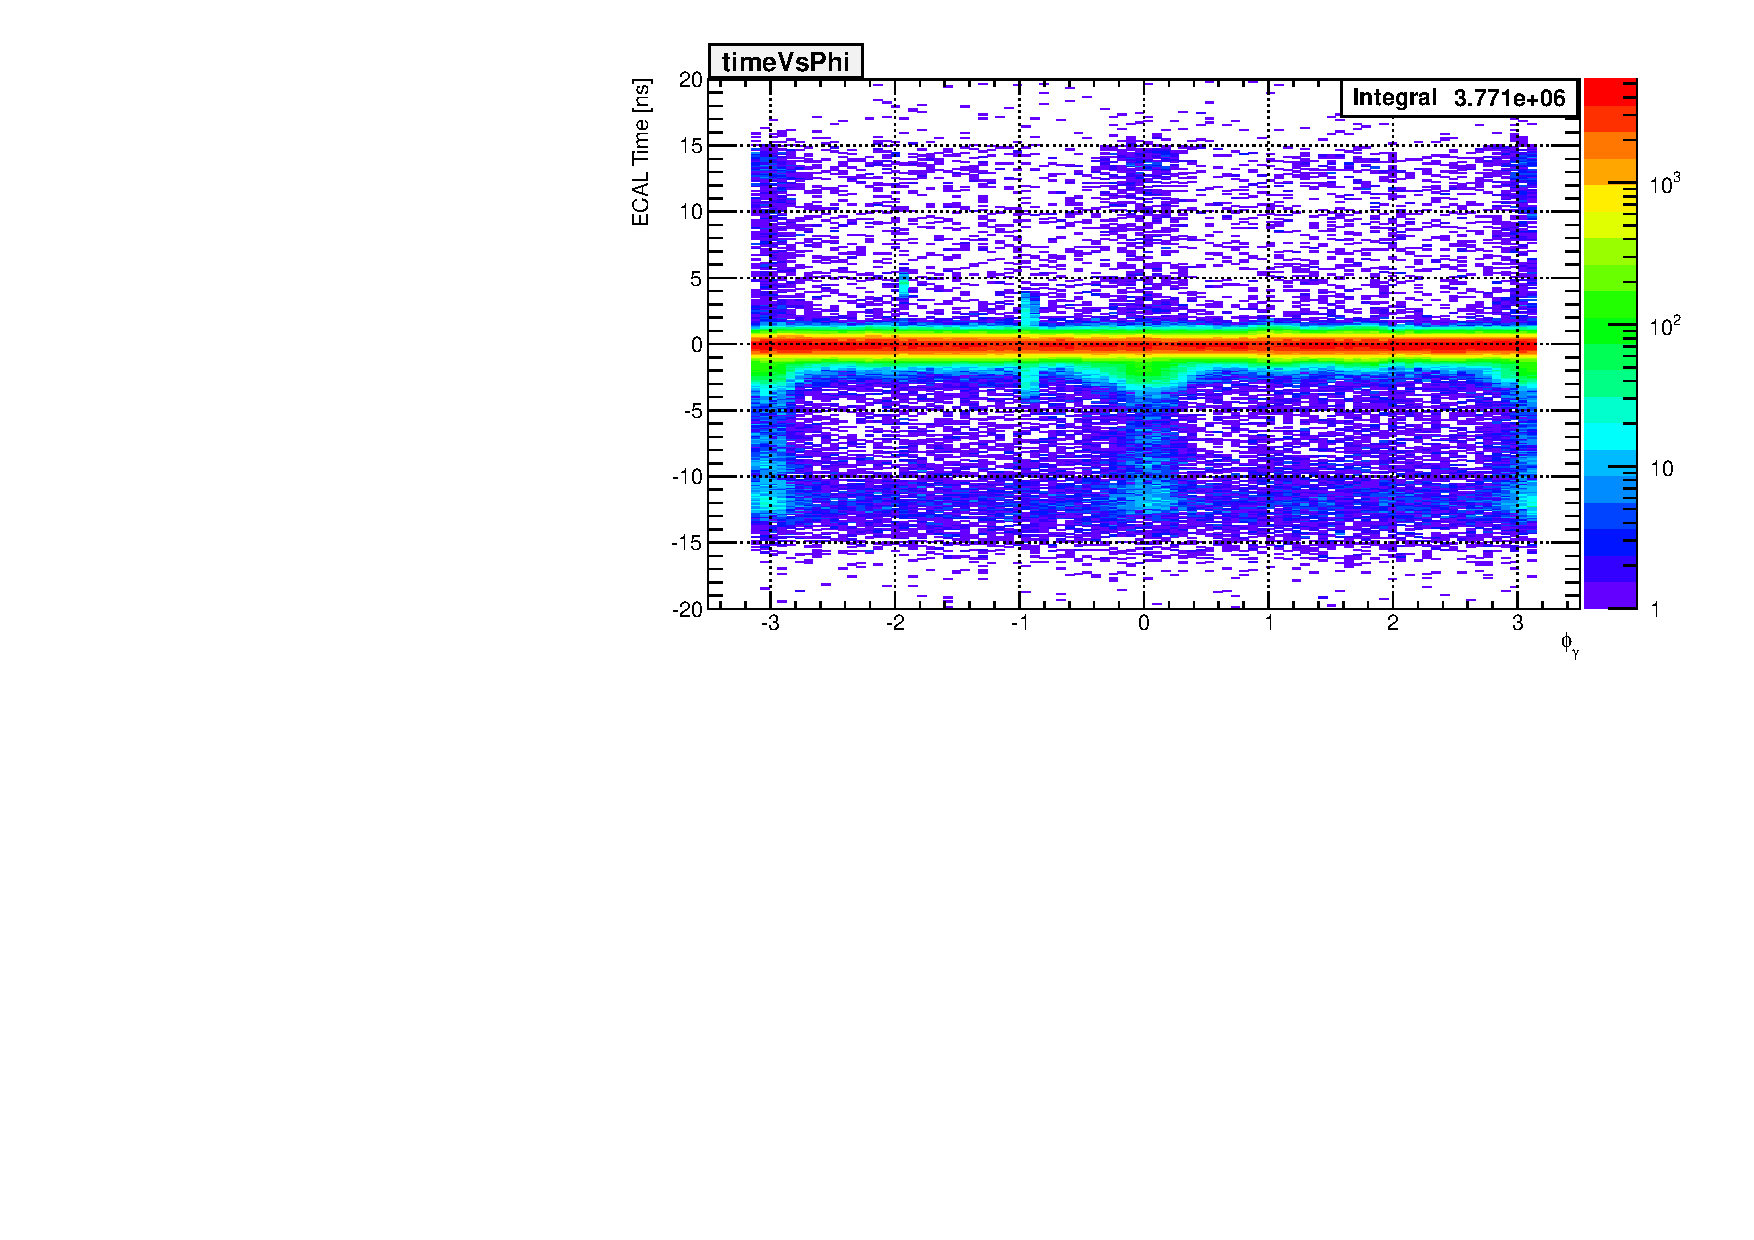
\includegraphics[height=6cm, width=0.5\textwidth]{THESISPLOTS/SinglePhotonDataSet-TimeVsPhiEB.pdf}
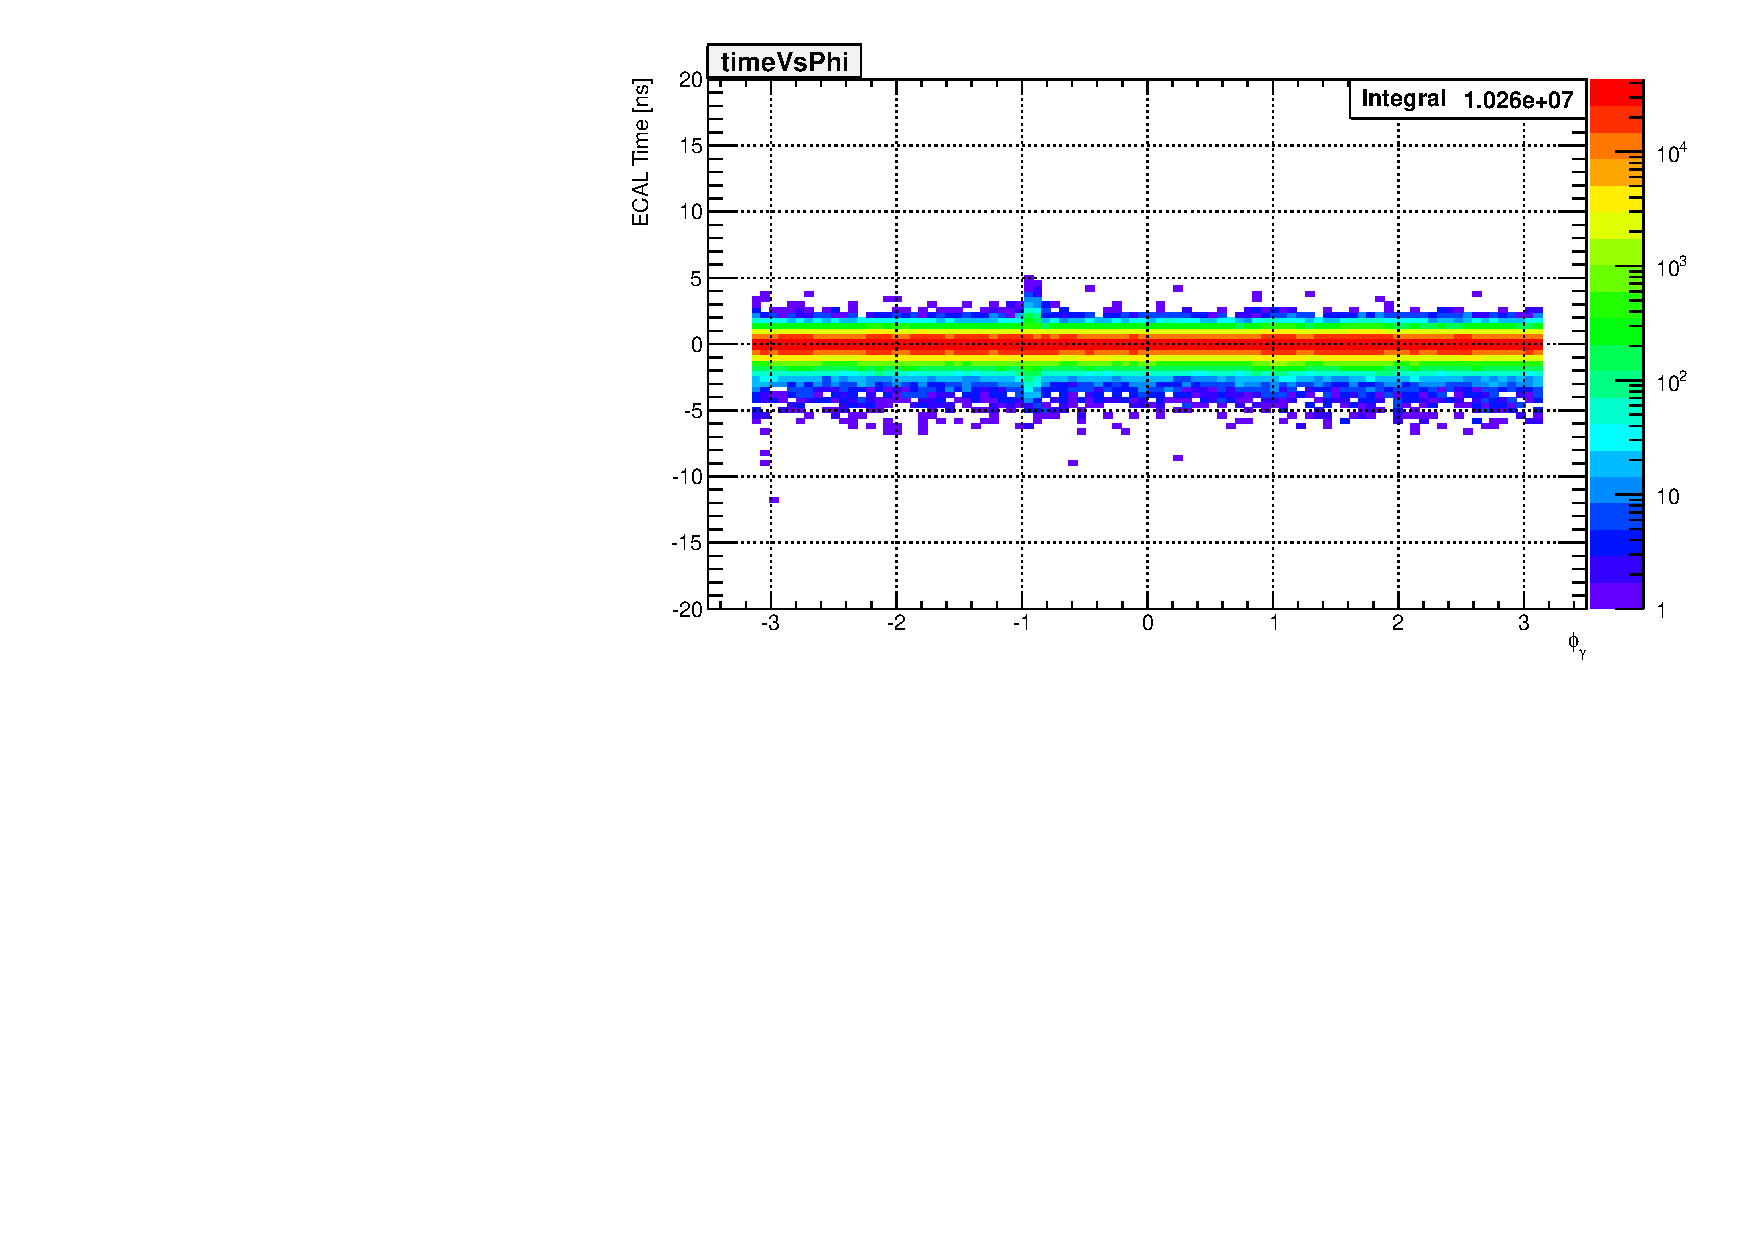
\includegraphics[height=6cm, width=0.5\textwidth]{THESISPLOTS/ZCandidates_TimeVsPhi.pdf}}
\captionof{figure}{ECAL time, $t_{\gamma}$ Vs $\eta_{\gamma}$(top) and $t_{\gamma}$ Vs $\phi$~(bottom) for photons from \texttt{SinglePhoton} dataset~(left) compared to electron candidates from the \texttt{DoubleElectron} dataset~(right). All photons or electron candidates are in barrel subdetector. Most of the photons with $\phi = 0, \pm \pi$ are halo photons which are not observed in the $Z$ boson candidate sample.}
\label{fig:Elec}
\end{center}

Figure \ref{fig:Zmass} shows the $Z$ boson mass reconstructed from the candidate electrons and timing of each electron for Signal~(\textit{top and blue}) and for our control sample~(\textit{bottom and red}).

\begin{center}
\centering
\mbox{
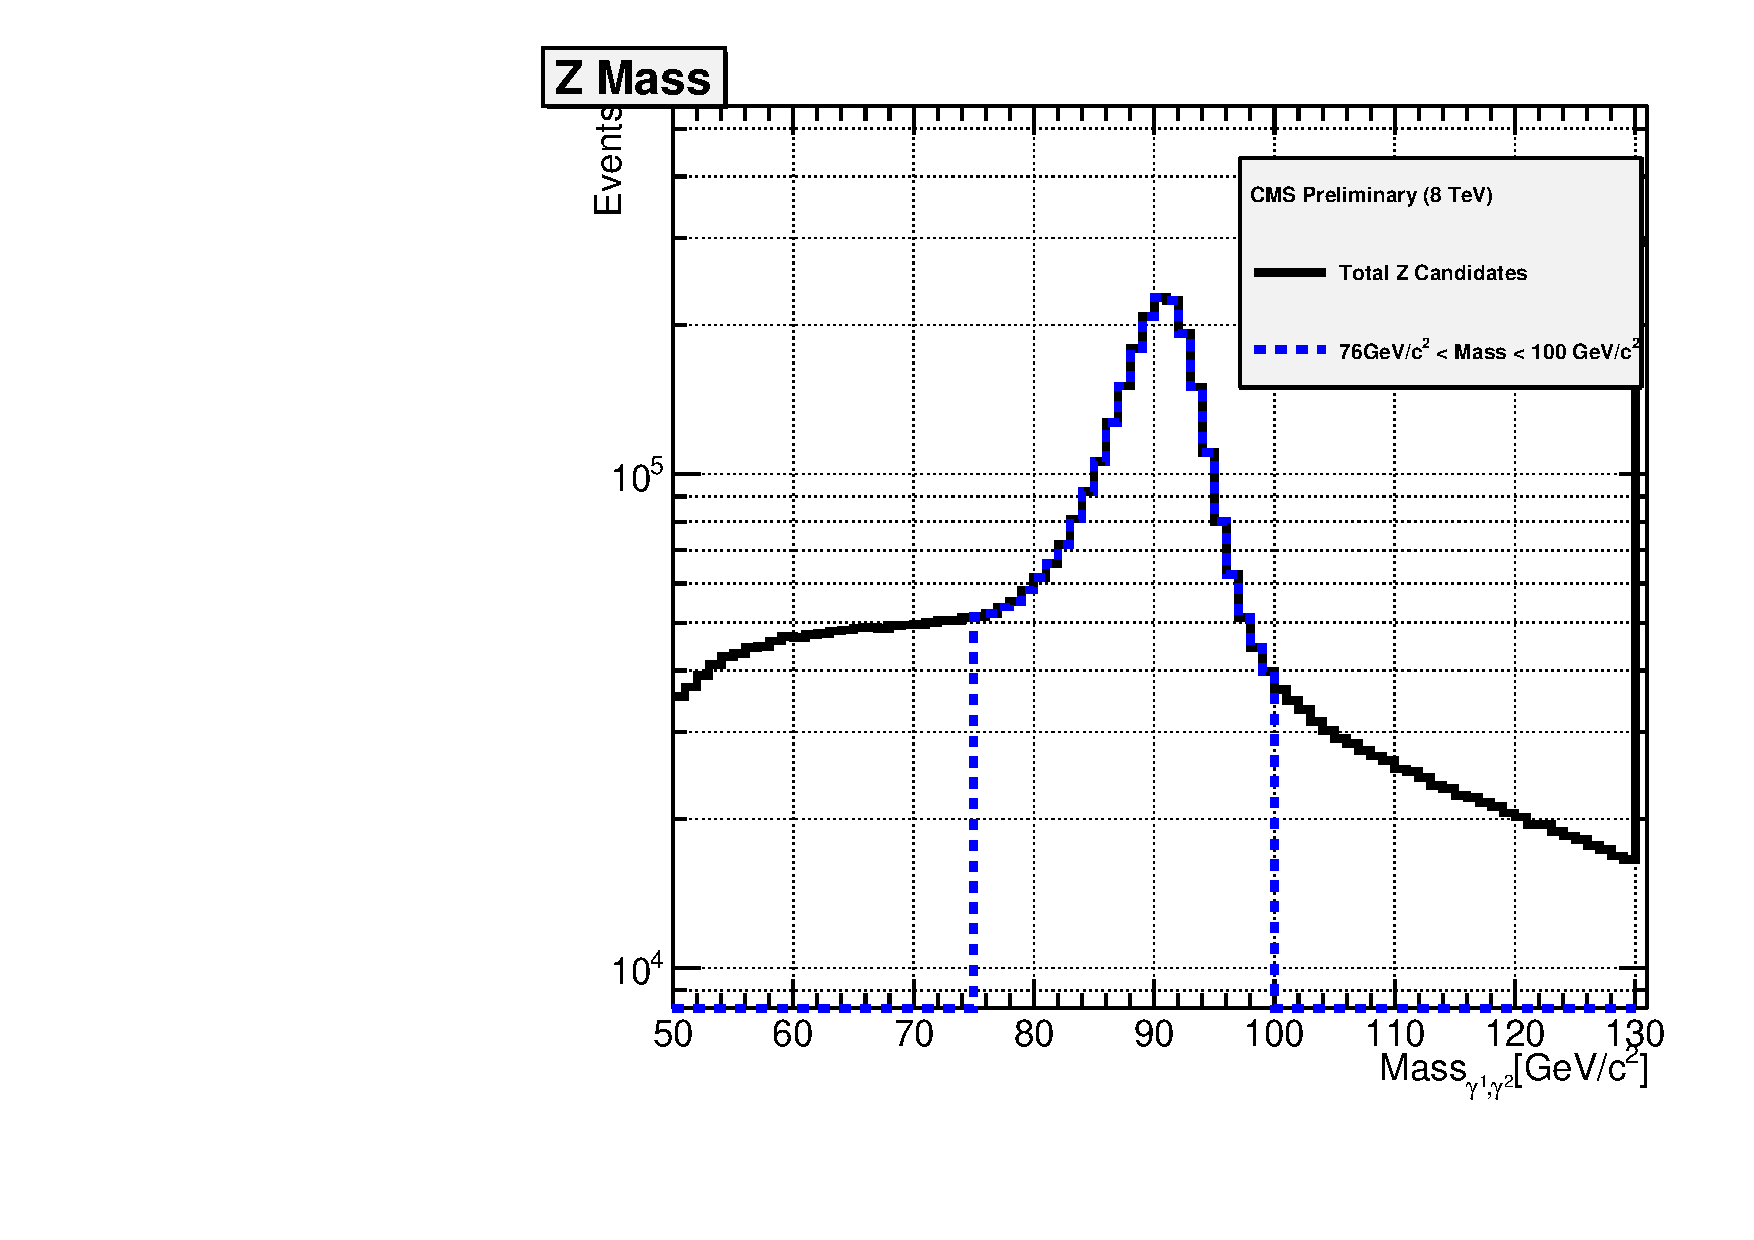
\includegraphics[height=6cm, width=0.5\textwidth]{THESISPLOTS/Z-CandidateOverLay-SignalMass.pdf}
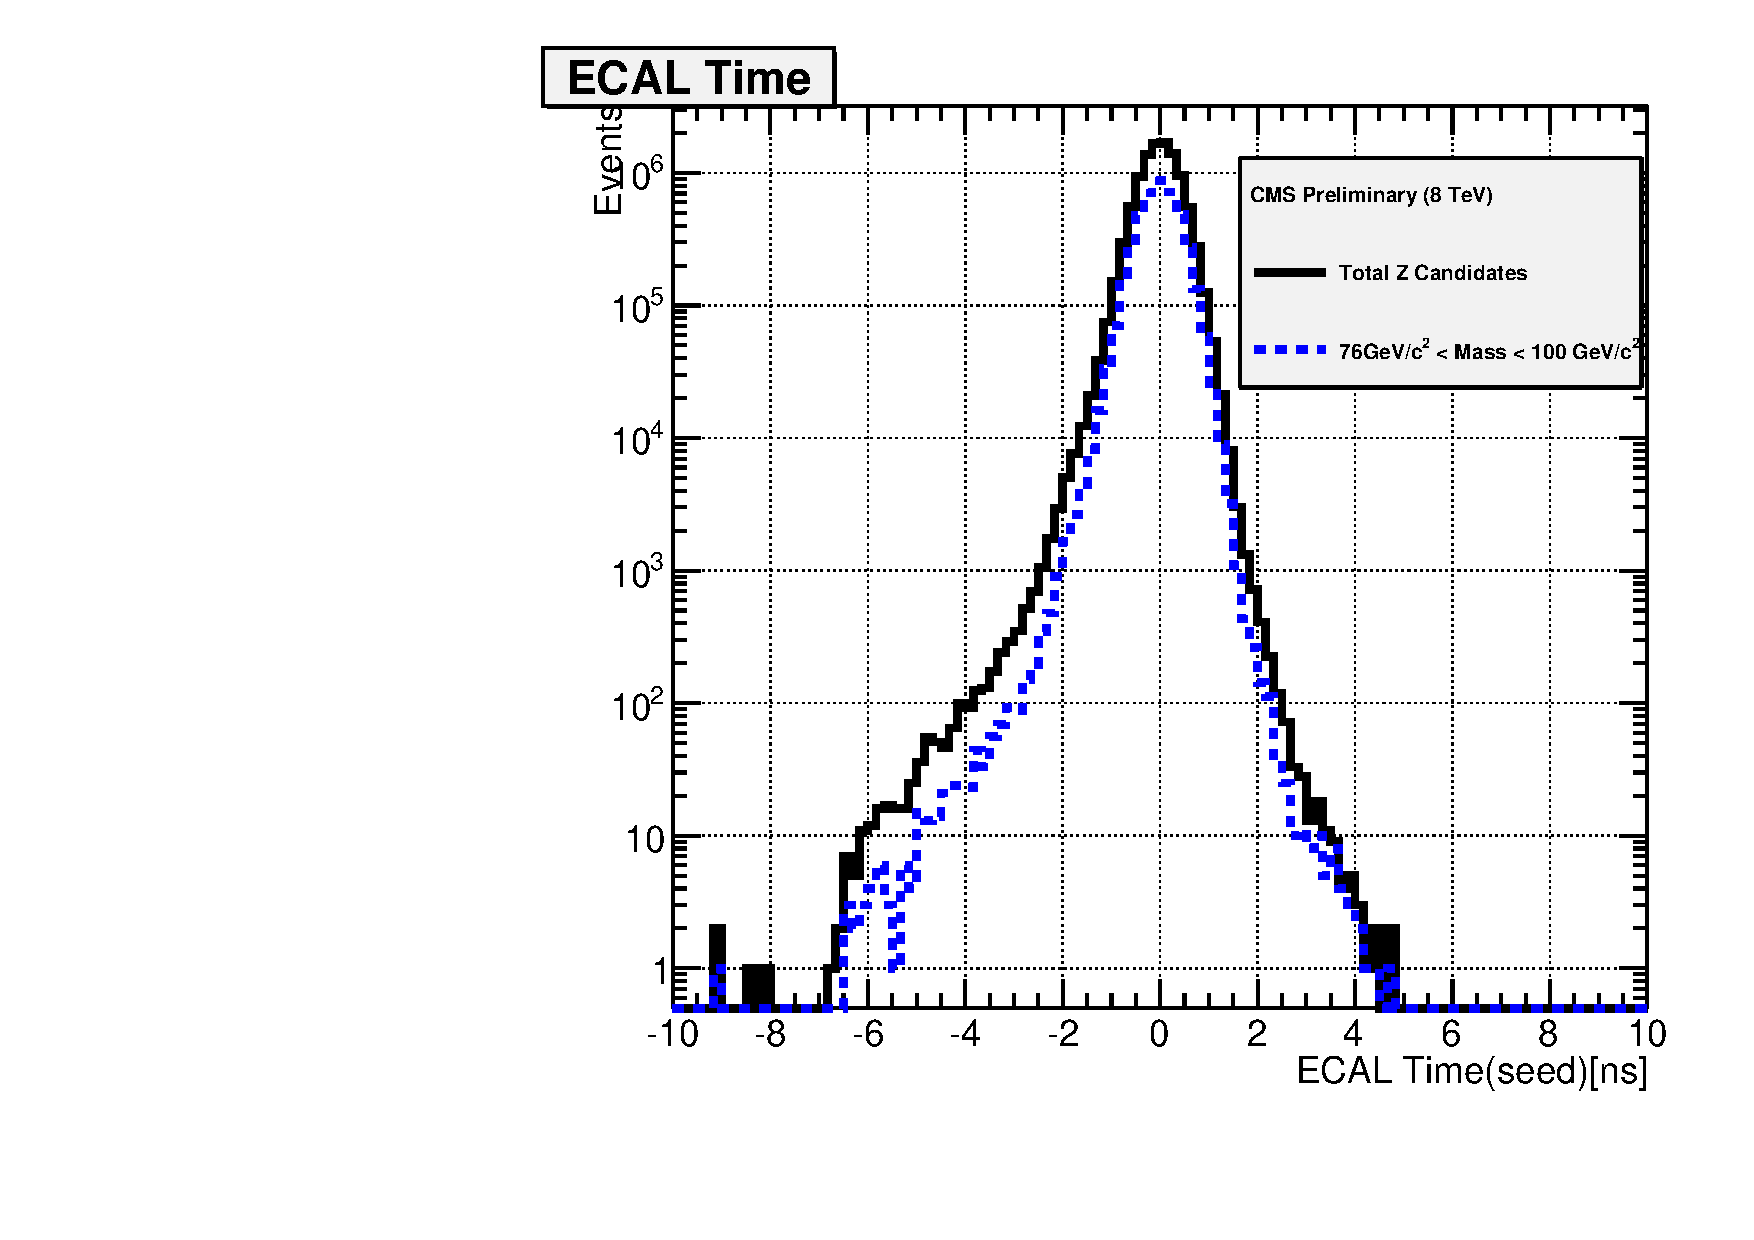
\includegraphics[height=6cm, width=0.5\textwidth]{THESISPLOTS/Z-CandidateOverLay-SignalTime.pdf}}
\mbox{
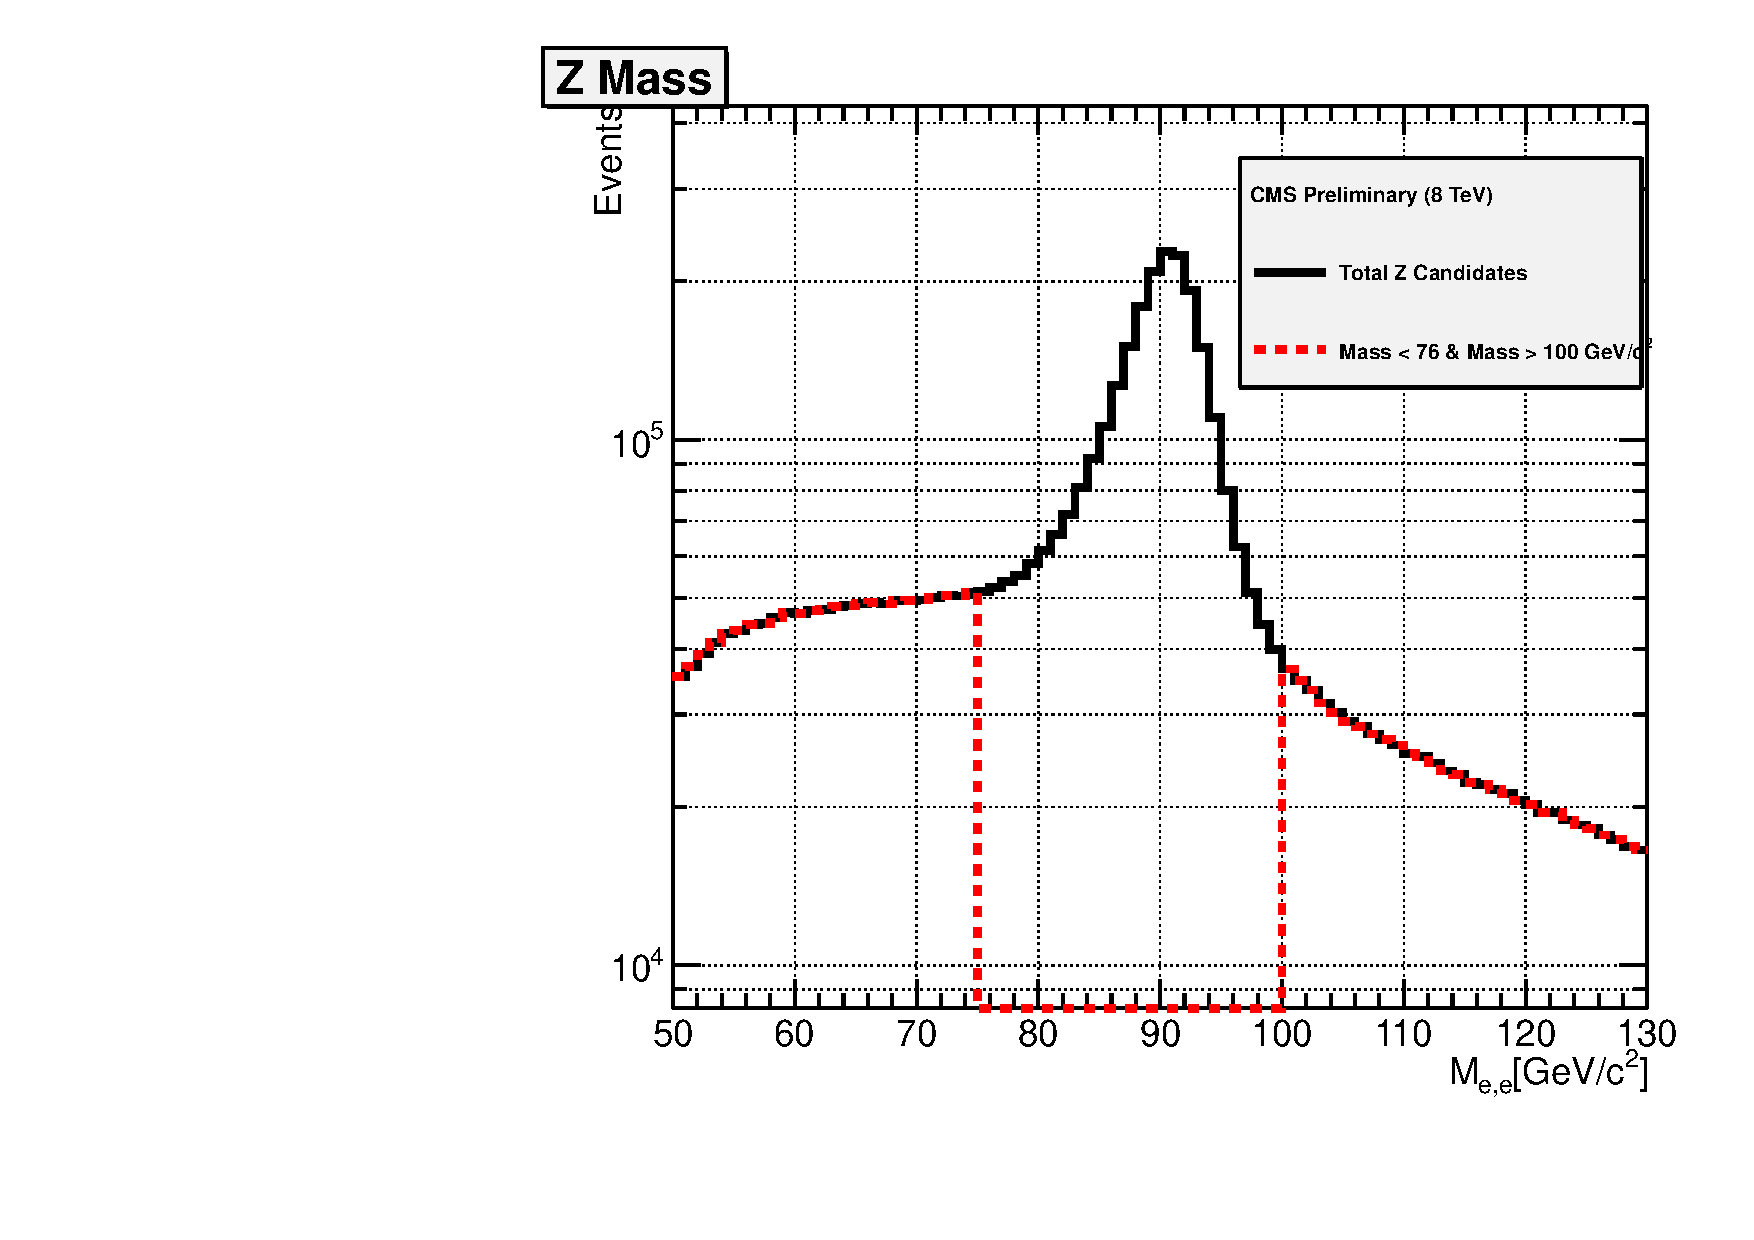
\includegraphics[height=6cm, width=0.5\textwidth]{THESISPLOTS/Z-CandidateOverLay-BackgroundMass.pdf}
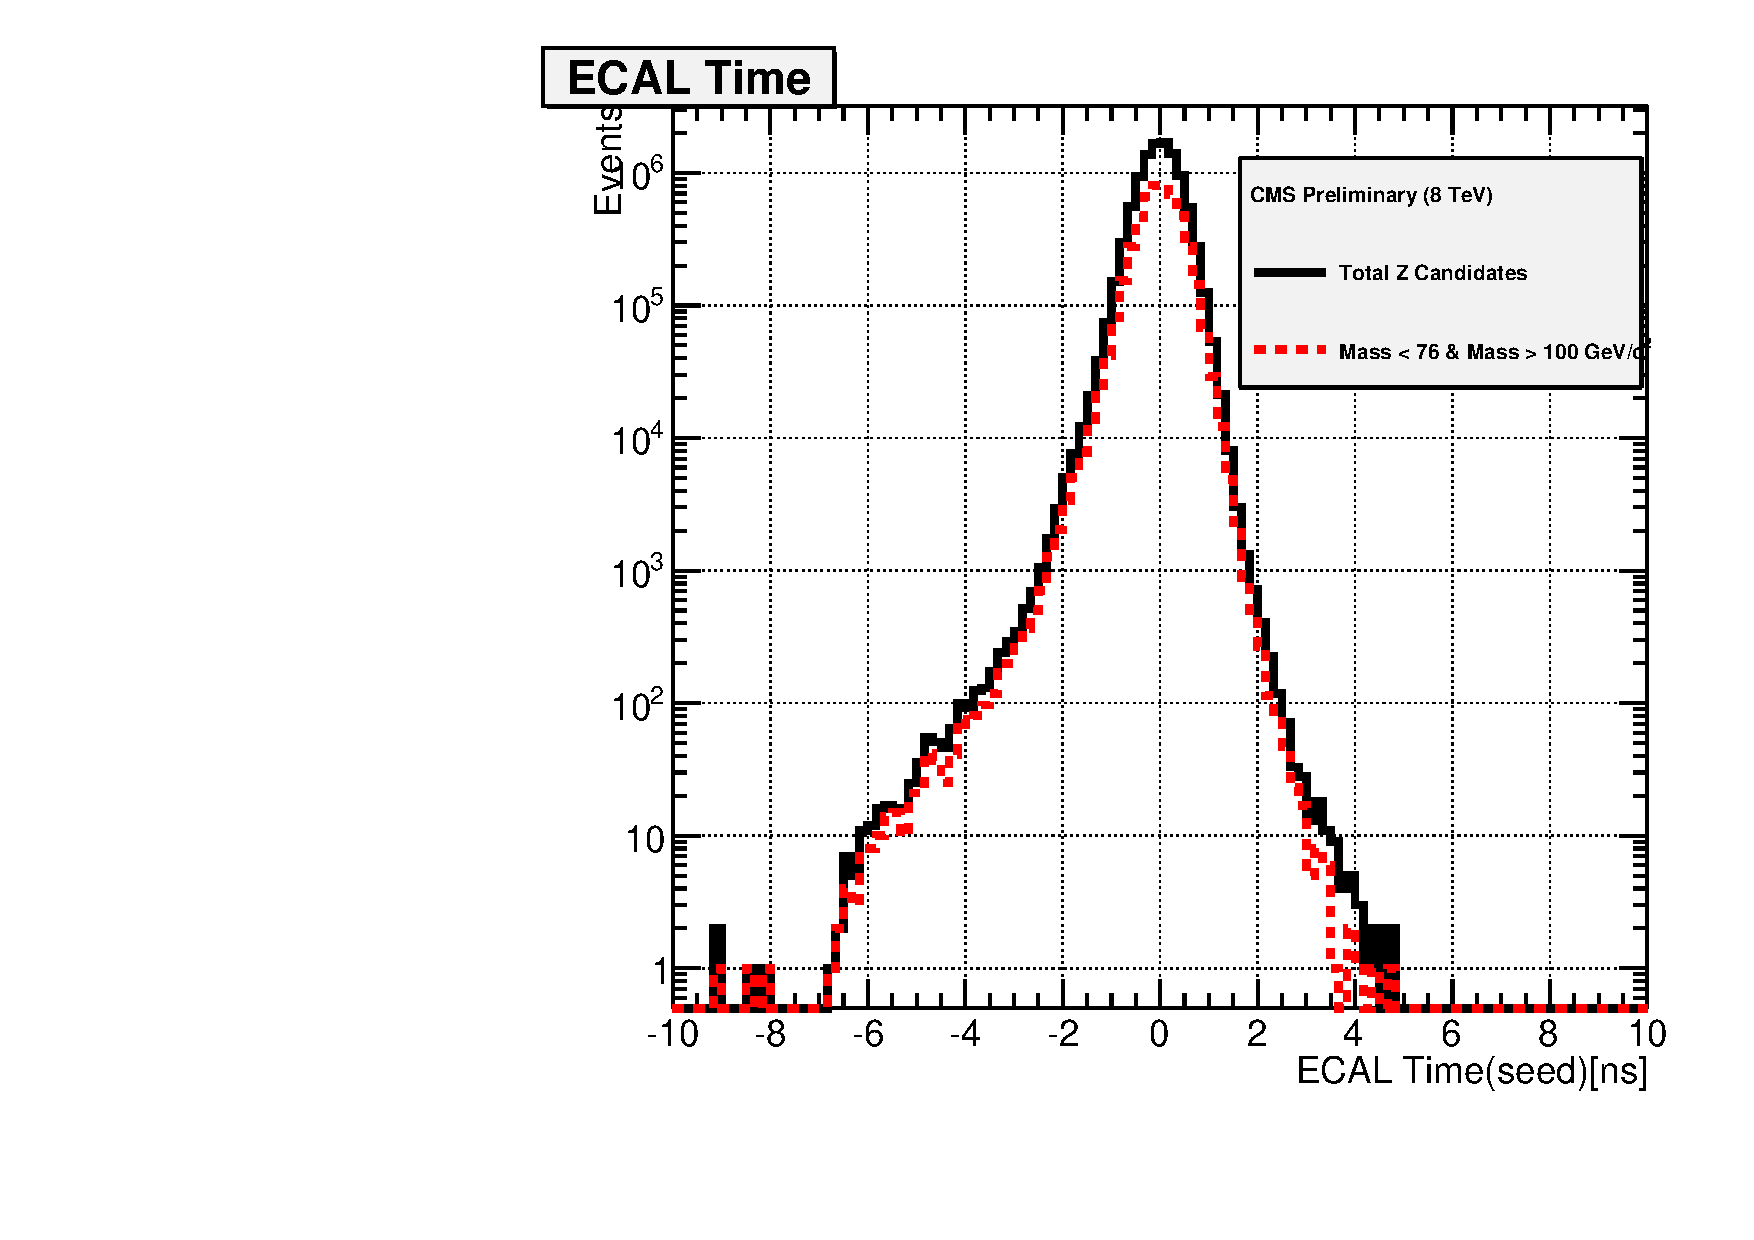
\includegraphics[height=6cm, width=0.5\textwidth]{/home/tensr/Documents/TEN-HEP-PHD-THESIS/PHD_THESIS/PHD/THESISPLOTS/Z-CandidateOverLay-BackgroundTime.pdf}}
\captionof{figure}{Di-electron candidate mass distribution and the time of both electrons for the signal \textcolor{blue}{$76 < m_{Z} < 100$}~\GeVcc $Z$ boson sample(left) and similar distributions from the Control~(\textcolor{red}{$50 < m_{Z} < 76$}~\GeVcc and \textcolor{red}{$ 100 < m_{Z} < 130$}~\GeVcc) sample~(right). Candidates events from the DoubleElectron dataset.}
\label{fig:Zmass}
\end{center}


Using the background $Z$ control sample, we estimate its contribution to out-of-time events using a simple scaling methods which can also be understood as an ABCD method. The method is applied as follows:
\begin{itemize}
\item Using a polynomial function, we fit the di-electron candidate mass distribution of the background control sample to extract a set of fit parameters,
\item Using these fit parameters to define our polynomial function, we use this function  to extract a scaling factor use to determine the true contribution of the background control region events in the signal region which in this case are $Z$ bosons with possible large ECAL timing, $|t| > 3$~ns.
\item We scale the background control sample timing distribution~(electrons time) using the extracted scale factor. This scale factor is defined as,   $$\displaystyle{\mbox{Scale Factor} = \frac{N}{M_{1} + M_{2}}}$$
\item By subtracting the scaled background control sample $Z$ candidates timing distribution from the signal sample $Z$ candidate timing distribution, we are left with the real $Z$ boson events whose electron time can fluctuate into larger timing region.
\item Comparing the total number of observe electron candidates with $t > 3$~ns to those  in-time, $|t| < 2$~ns, their ratio i.e $ N_{t > 3~ns}/ N_{|t| < 2.0~ns}$ gives us an estimate of the possible genuine electromagnetic objects from collision with large ECAL timing. 
\end{itemize}  

A simple picture showing the above procedure with distributions is shown in figure \ref{fig:collZ}.

\begin{center}
\centering
\mbox{
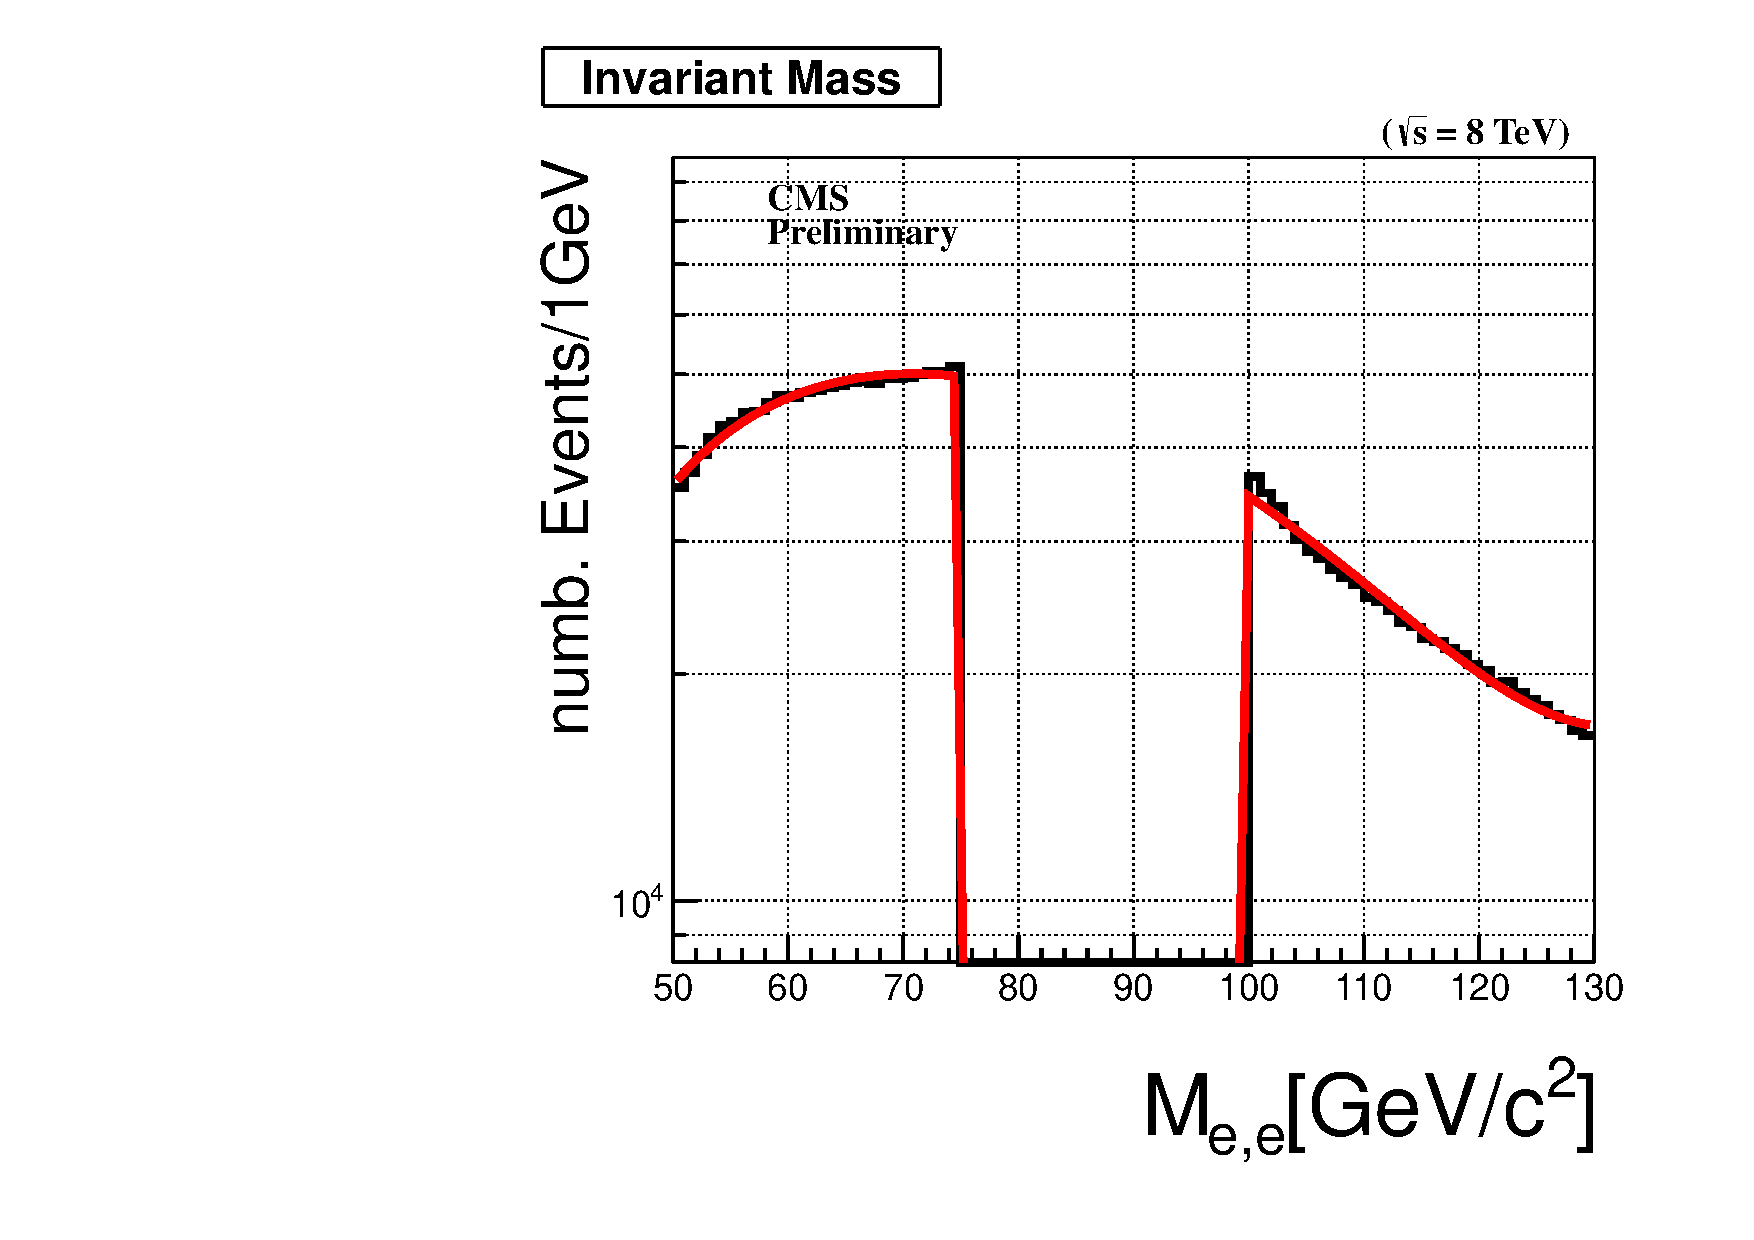
\includegraphics[height=7cm, width=0.5\textwidth]{THESISPLOTS/Uncleaned-di-Photon-ZMass-Fit-DoubleElectron-Run2012A.pdf}
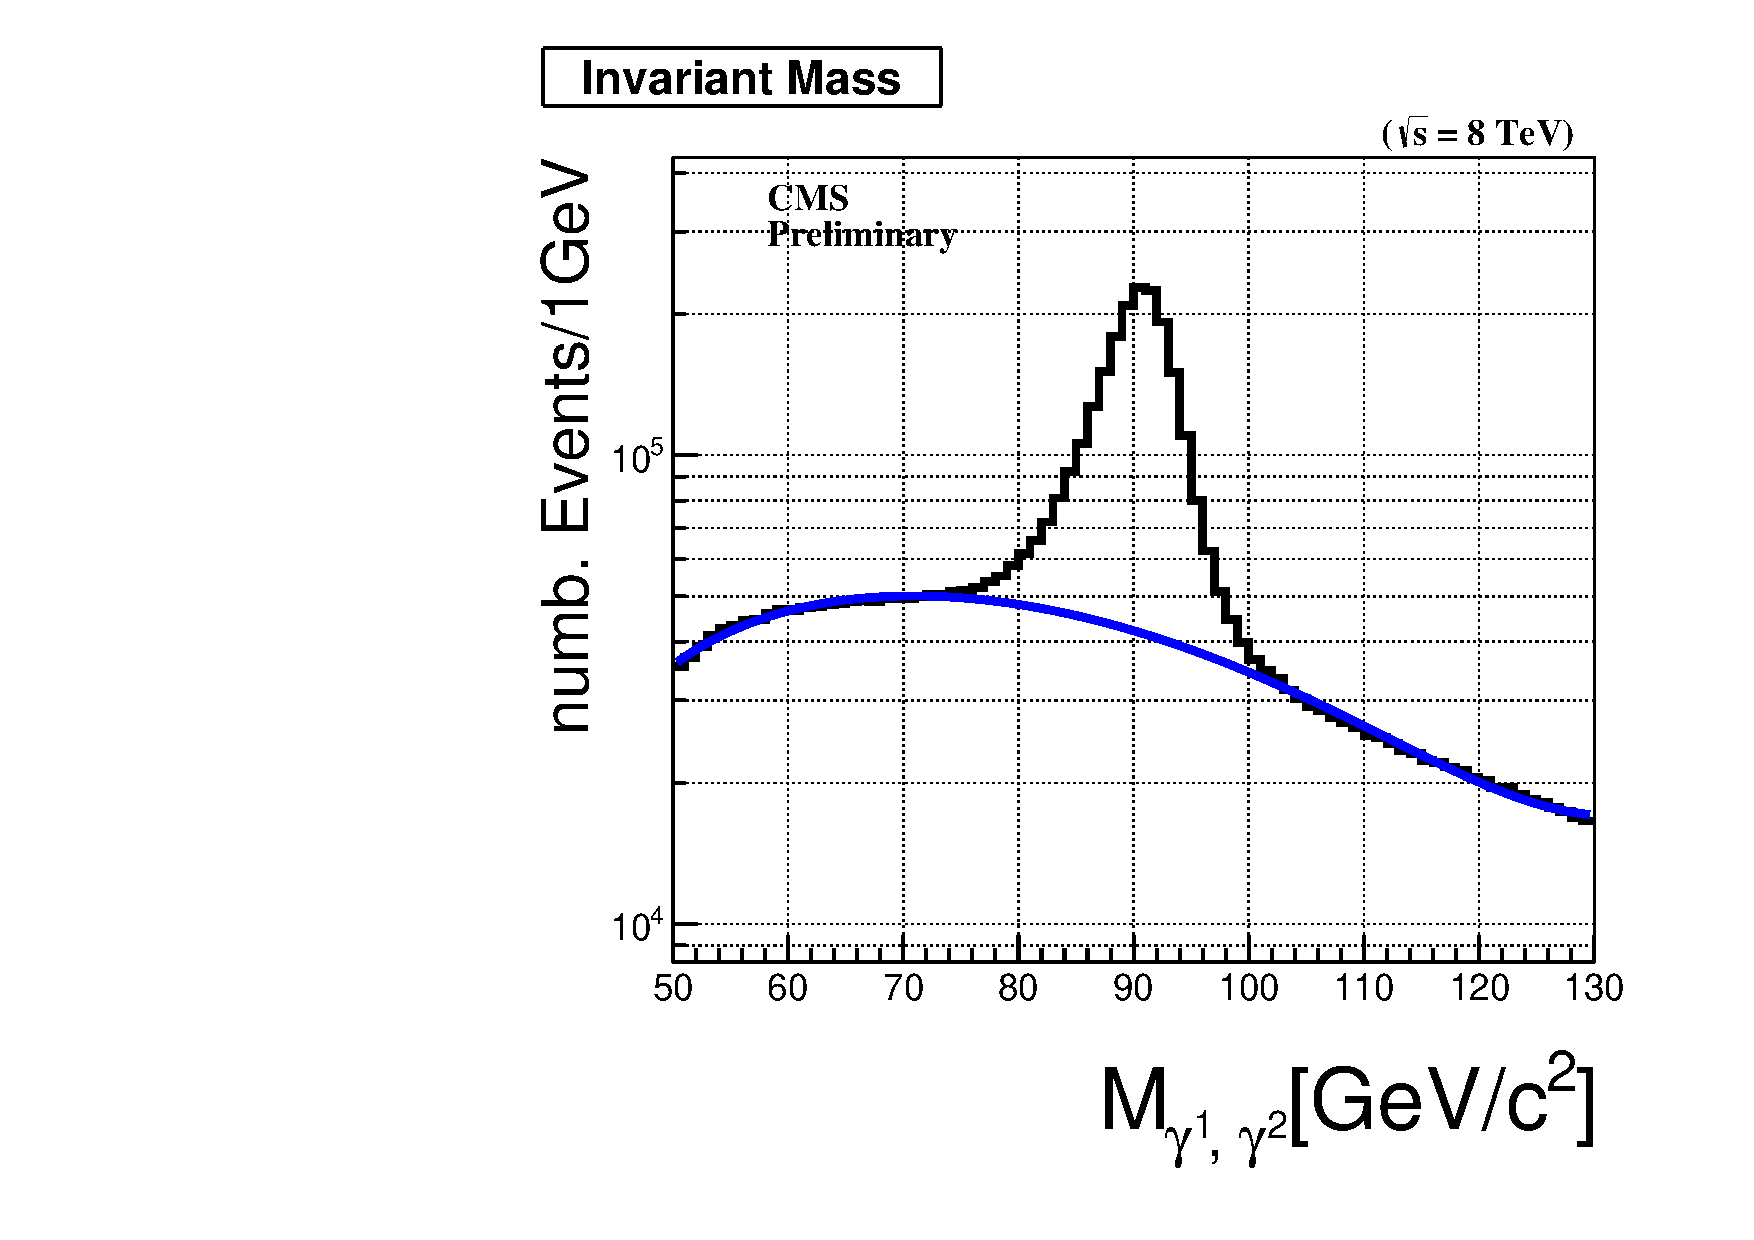
\includegraphics[height=7cm, width=0.5\textwidth]{THESISPLOTS/Background_In_ZMass-From-Di-Photon.pdf}}
\mbox{
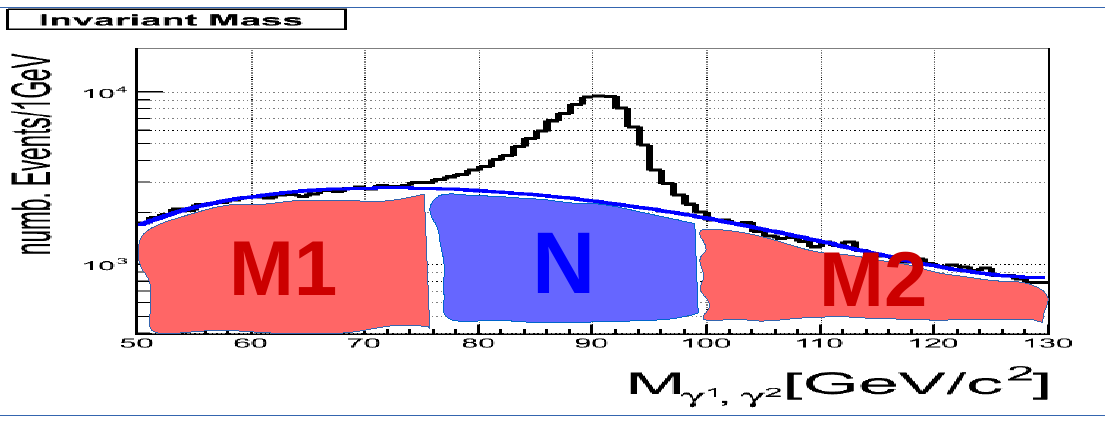
\includegraphics[height=8cm, width=0.8\textwidth]{THESISPLOTS/ZBackground_SF.png}
%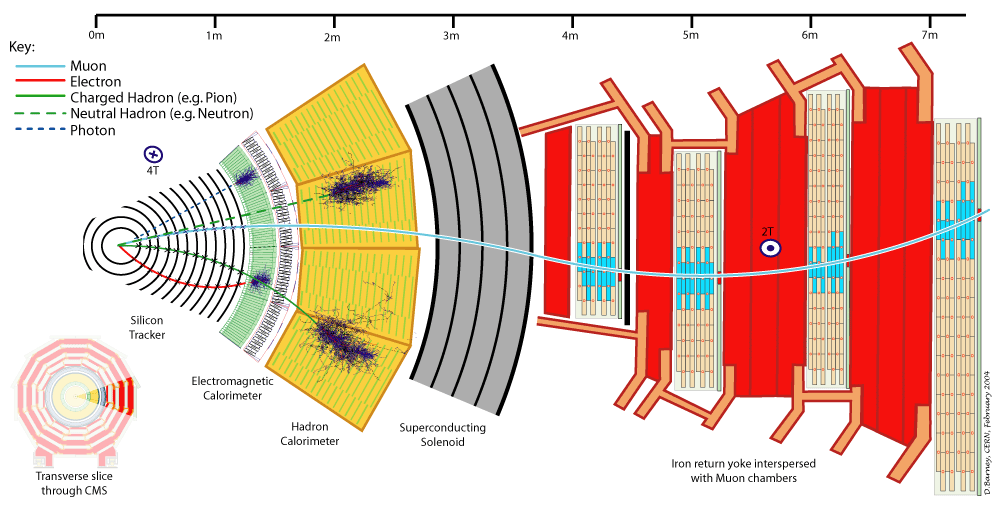
\includegraphics[height=6cm, width=0.5\textwidth]{THESISPLOTS/CMS_Slice.png}
}
\captionof{figure}{\textit{Top}: Control sample~(left) and signal sample~(right) of di-electron candidate mass distribution. \textit{Bottom:} Figure showing definition of scale factor use in estimating the contributions from control sample in signal sample.}
\label{fig:collZ}
\end{center}

The result of the final timing distribution of genuine $Z$ boson events  can be seen in figure \ref{fig:Ztime}. It is not difficult to see that the ratio $ N_{t > 3~ns}/ N_{|t| < 2.0~ns}  < 10^{-5}$ confirming that indeed the contribution  of electromagnetic objects with large timing $t >3$~ns is negligible thus confirming that most collision events contain photons which are mostly in-time, $|t| \leq 2$~ns. A simple cut on the \MET, $\MET > 60$~GeV will further reduce this ratio to $0$ as assumed in our above background estimation.
\begin{center}
\centering
%\mbox{
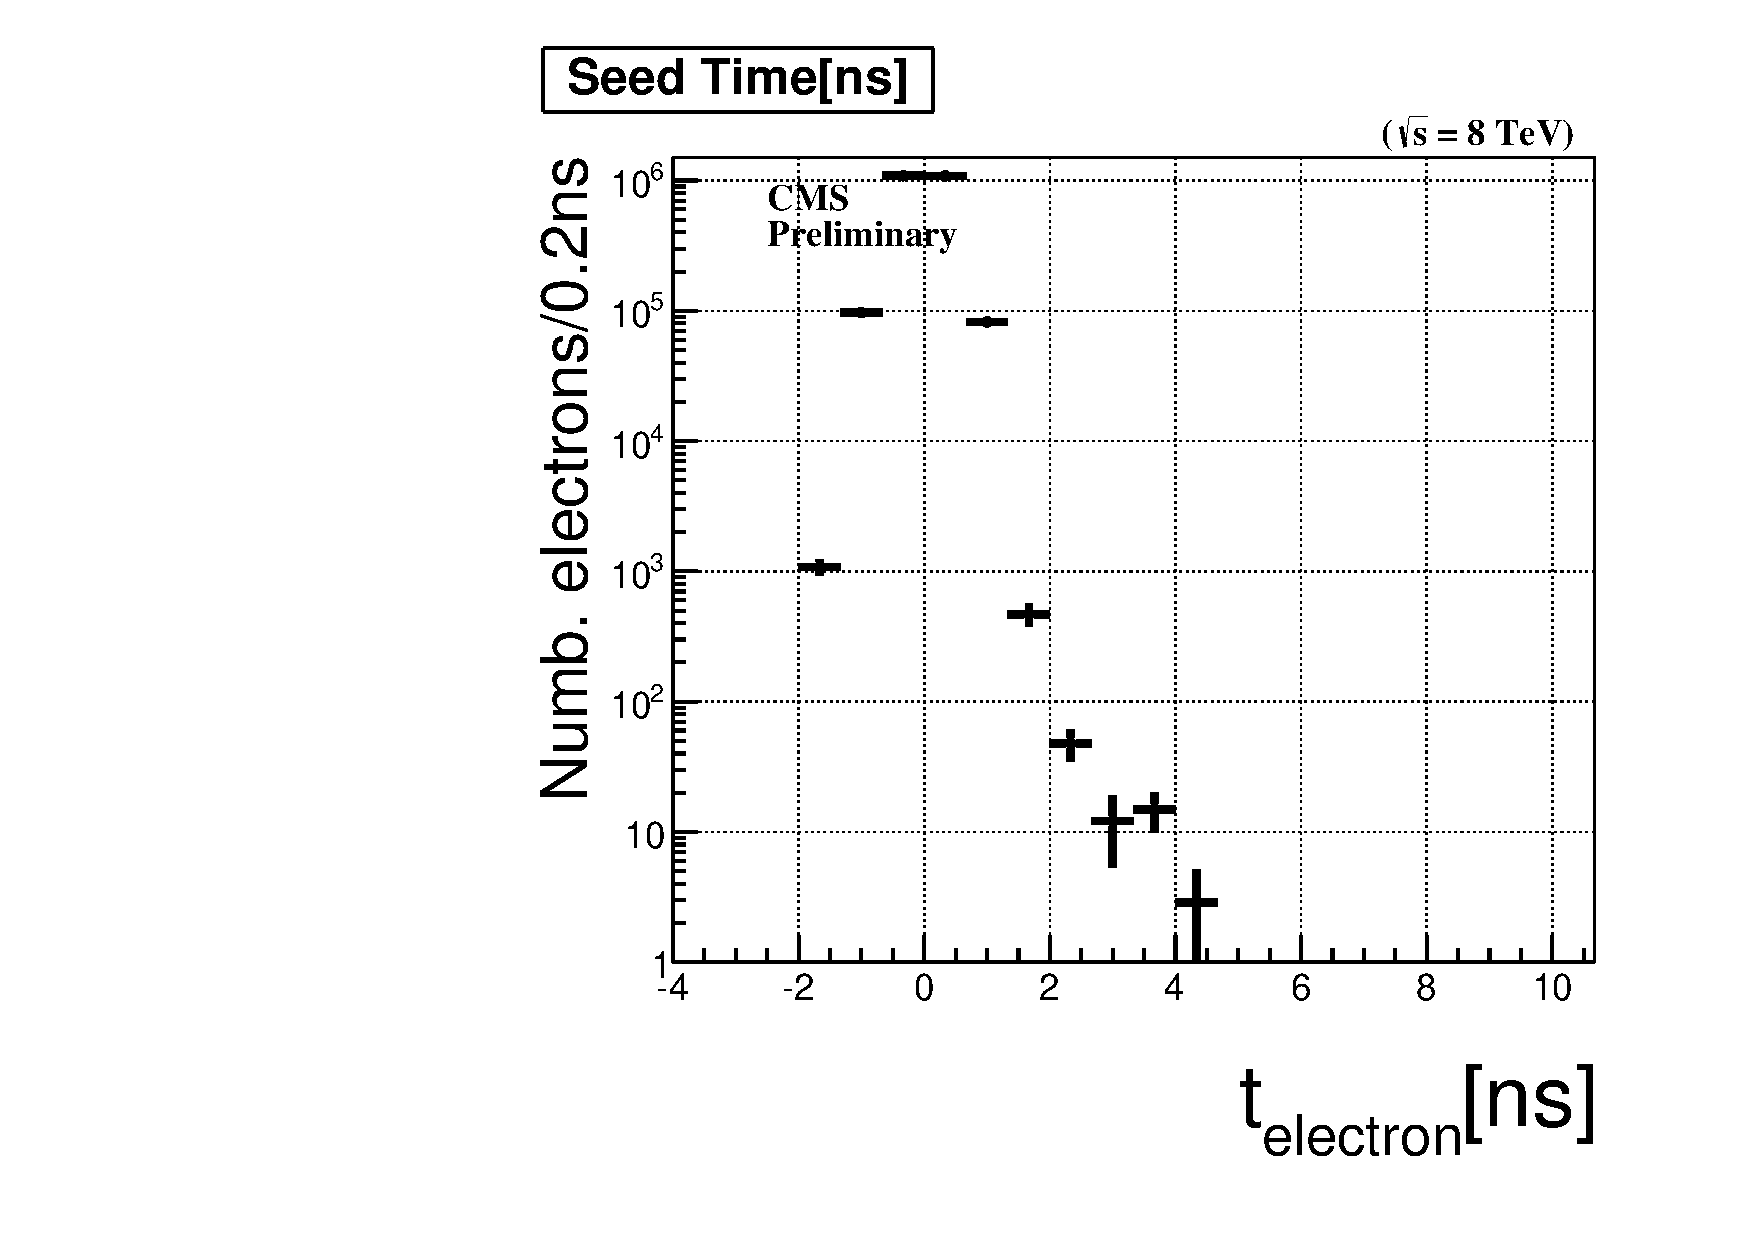
\includegraphics[height=7cm, width=0.7\textwidth]{THESISPLOTS/Seed-Time-From-Uncleaned-di-photon-Mass-Fit-DoubleElectron-Run2012A.pdf}
%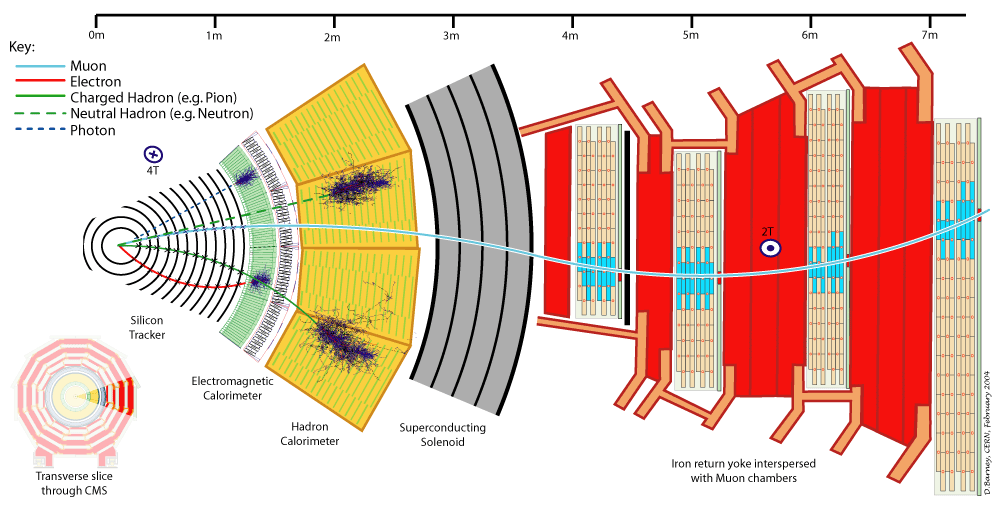
\includegraphics[scale=0.2]{THESISPLOTS/CMS_Slice.png}
\captionof{figure}{Timing distribution of genuine $Z$ bosons after background contribution has been subtracted.}
\label{fig:Ztime}
\end{center}


\section{Results}
Finally, we perform our background estimation on our true signal samples which are events with at least 2 jets, at least one high $\pt > 80~GeV/c$ isolated photon with ECAL time  $ 3.0 < t_{\gamma} < 13.0$~ns or $ -10.0 < t_{\gamma} < -3.0$~ns and ${\ETslash}^{\gamma}$~~$ > 60$~GeV, ${\ETslash}$~~$ > 60$~GeV.

We observed $1$ event and expected $0.0888 ^{+0.1869}_{-0.0444}$ background events within our statistical uncertainties. The complete result is shown in table \ref{tab:RF} and in table \ref{tab:RESULT} we show the number of GMSB SPS8 signal events  passing our final selection for $\Lambda=180$~\TeV and different $c\tau$ values of the neutralino.

\begin{center}
\centering
\begin{tabular}{|c| c| c|}
%\mbox{Fake Rate }
\hline
\bfseries{Non-Collision} & \bfseries{ ${\ETslash}^{\gamma}$~~$ < 60$~\GeV} & \bfseries {${\ETslash}^{\gamma}$~~$ > 60$~\GeV} \\
\hline
 $3.0 < t_{\gamma} < 13.0$~ns & \textsf{$C$}($0$) & ~\textsf{$D$}(\textcolor{blue}{$1$}) \\
 $-10.0 < t_{\gamma} < -3.0$~ns & \textsf{$A$}($5$) & ~\textsf{$B$}($1$) \\
\hline \hline

\bfseries{Collision} & \bfseries{ ${\ETslash}$~~$ < 60$~\GeV} & \bfseries {${\ETslash}$~~$ > 60$~\GeV} \\
\hline 
 $3.0 < t_{\gamma} < 13.0$~ns & \textsf{$D^{\prime}$}($5$) & ~\textsf{D} \textcolor{red}{$0.0888 ^{+0.1869}_{-0.0444}$} \\
 $-2.0 < t_{\gamma} < 2.0$~ns & \textsf{$F^{\prime}$}($657663$) & ~\textsf{$F$}($30242$) \\
 $-10.0 < t_{\gamma} < -3.0$~ns & \textsf{$B^{\prime}$}($1$) & ~\textsf{$B$} $0.23 ^{+0.092}_{-0.118}$) \\
\hline\hline 
\end{tabular}
\captionof{table}{Result of observed events and estimated background from signal sample, events with at least $2$-jets. Numbers in bracket represent our observed events while numbers not is bracket are our expected background events using \textsf{ABCD} method.}
\label{tab:RF} 
\end{center}



\begin{center}
%\begin{table}[ht]
%\renewcommand\arraystretch{1.2}
\centering
\begin{tabular}{c c}
\hline
\bfseries{SPS8 GMSB Signal} & \bfseries {Number of Events}\\
\hline \hline
%\texttt{GMSB(SPS8)}~($\Lambda=180$~TeV,$c\tau=93$~mm) & $000.00 \pm 0.000$ \\
%\texttt{GMSB(SPS8)}~($\Lambda=180$~TeV,$c\tau=185$~mm) & $000.00 \pm 0.000$ \\
\texttt{GMSB(SPS8)}~($\Lambda=180$~TeV,$c\tau=250$~mm) & $0.2096$ \\
\texttt{GMSB(SPS8)}~($\Lambda=180$~TeV,$c\tau=500$~mm) & $4.5423$ \\
%\texttt{GMSB(SPS8)}~($\Lambda=180$~TeV,$c\tau=733$~mm) & $000.00 \pm 0.000$ \\
\texttt{GMSB(SPS8)}~($\Lambda=180$~TeV,$c\tau=1000$~mm) & $6.3646$ \\
%\texttt{GMSB(SPS8)}~($\Lambda=180$~TeV,$c\tau=1076$~mm) & $000.00 \pm 0.000$ \\
%\texttt{GMSB(SPS8)}~($\Lambda=180$~TeV,$c\tau=1444$~mm) & $000.00 \pm 0.000$ \\
\texttt{GMSB(SPS8)}~($\Lambda=180$~TeV,$c\tau=2000$~mm) & $6.3968$ \\ %\texttt{GMSB(SPS8)}~($\Lambda=180$~TeV,$c\tau=3000$~mm) & $000.00 \pm 0.000$ \\
\texttt{GMSB(SPS8)}~($\Lambda=180$~TeV,$c\tau=4000$~mm) & $6.1442$ \\
\texttt{GMSB(SPS8)}~($\Lambda=180$~TeV,$c\tau=6000$~mm) & $4.6498$ \\
\texttt{GMSB(SPS8)}~($\Lambda=180$~TeV,$c\tau=12000$~mm) & $2.918$ \\
\hline \hline
\end{tabular}
\captionof{table}{Final number for $\Lambda = 180$~\TeV GMSB SPS8 MC signal events  events passing our selection cuts.}
\label{tab:RESULT}
%\end{table}
\end{center}



\subsection{Systematics Studies}
The different sources of systematics which affect this analysis and the estimated contribution of each identified systematics is used in the calculation of the upper limit on observed signal cross-section is shown in table \ref{tab:SYST}.
The systematic uncertainty on luminosity measurement has the recommended value of $2.2$\%. The uncertainty for the jet energy scale correction has also been measured using the standard CMSSW tool by \cite{JES}. The uncertainty on the photon energy scale in barrel was estimated to be 1.0\% and based on the final-state radiation~(FSR) in $Z\rightarrow \mu\mu\gamma$ events \cite{PES}. The uncertainty from pardon density functions~(PDF) evaluated using the re-weighting technique and Master equation of CTEQ65 model set described in \cite{PDF}. The uncertainty on the \MET resolution uses a conservative estimate from \cite{METRES}. The uncertainty on the ECAL timing obtained be comparing the peak in the timing distribution between $\gamma +$ jet sample and data events with time $|t| < 2$~ns to be of the order of 200~ps per event and from a study of high \pt photons beyond gain transitions and has been agreed by ECAL DPG to be a conservative estimate. Another important source of systematics is in the selection of the background control samples and estimation and individual systematics in the tagging and miss-tagging of non-collision background and also with the estimation of background contributions from collisions. All these separate systematics contributions have been combined into a single background estimation systematics referred to as background estimation systematics. The summary of every systematics in shown in table \ref{tab:SYST}. 



\begin{center}
%\begin{table}[ht]
%\renewcommand\arraystretch{1.2}
\centering
\begin{tabular}{c c}
\hline
\bfseries{Source} & \bfseries {Uncertainty on $\sigma^{Exp}_{UL}$}(\%)\\
\hline
\texttt{Photon energy scale}~(1.0\%)  & $< 3.0$\% \\
\texttt{Jet energy scale}  & $< 0.05$\% \\
\texttt{Jet energy resolution}~(10\%) &$ < 1.90$\% \\
\texttt{PDF uncertainty}~(10\%) & $< 1.70$\% \\
\texttt{\MET resolution}~(10\%) & $ <2.8$\%  \\
\texttt{ECAL time uncertainty}~(0.5~ns) & $<5.0$\% \\
\hline
\texttt{Background estimation uncertainty}~(50.0) &$<41.0$\% \\
\hline 
\texttt{Luminosity}~(4.5\%) & $< 2.2$\% \\
\hline
\end{tabular}
\captionof{table}{Summary of systematic uncertainties on the signal~(top), background~(middle) and machine~(bottom) as used in the $\sigma_{UL}$ calculation.}
\label{tab:SYST}
%\end{table}
\end{center}



\label{Search_Analysis_chapter}